\documentclass[paper=a4wide, fontsize=11pt]{report}	 % A4 paper and 11pt font size
\usepackage[svgnames]{xcolor} % Using colors
\usepackage{xurl} %xurl en vez de url para urls largas
\usepackage[hidelinks]{hyperref}
\usepackage[utf8]{inputenc}
\renewcommand\thechapter{\Roman{chapter}}
\usepackage[spanish]{babel} % ponerlo en español
\usepackage{todonotes} % para poner notitas de colores
\usepackage{fancyhdr} % Needed to define custom headers/footers
\usepackage[a4paper, left=30mm, right=30mm, top=2.5cm, bottom=2.5cm, footskip=1.2cm]{geometry}  % Changing size of document
\usepackage{braket}
\usepackage{tabularx}
\usepackage{multirow}
\usepackage{nicematrix}
\usepackage[numbers]{natbib}
\usepackage{subcaption}
\usepackage{tabularx, makecell, booktabs}
\usepackage{textcmds}
\usepackage{color}
\usepackage{listings}
\usepackage{tabularray}
\usepackage{setspace} % Paquete para ajustar el interlineado
\definecolor{lightgray}{rgb}{.9,.9,.9}
\definecolor{darkgray}{rgb}{.4,.4,.4}
\definecolor{purple}{rgb}{0.65, 0.12, 0.82}
\usepackage{hyperref}
\hypersetup{
    colorlinks=true, % activa el color
    linkcolor=black, % color de los enlaces internos
    filecolor=magenta, % color de los enlaces a archivos
    urlcolor=blue % color de los enlaces URL
}
%%%%%% Setting up the style

\pagestyle{fancy} % Enables the custom headers/footers

\lhead{} \rhead{} % Headers - all  empty



\title{
{\Huge \textbf{Proyecto: 
\\ Sistemas de Información 2}}\\
\vspace{1cm}
\midrule
\vspace{1cm}
\text{Pablo Angusto\quad\href{mailto:842255@unizar.es}{842255@unizar.es}}\\
\text{Miguel Aréjula\quad\href{mailto:850068@unizar.es}{850068@unizar.es}}\\
\text{Grupo E}\\

\includegraphics[width=6cm]{logo.png}\\
\date{13 de mayo de 2024}\\



}


\cfoot{\color{Black} \thepage}

\renewcommand{\headrulewidth}{0.0pt} % No header rule
\renewcommand{\footrulewidth}{0.4pt} % Thin footer rule
\renewcommand{\thesection}{\arabic{section}} % para que los títulos no salgan en 0.1 ...

\setcounter{secnumdepth}{3}
%%%%%% Starting the document
\setlength\parindent{0pt} % No indentar los párrafos
\begin{document}
\large
\onehalfspacing
\maketitle % Print the title

\newpage
\section{Resumen Ejecutivo}
\paragraph{}
El presente documento presenta una evaluación detallada de la implementación de Odoo, un sistema de gestión empresarial de código abierto, en UZ-On-Marketing. Con el objetivo de optimizar la gestión de sus recursos y procesos, la empresa ha optado por esta solución modular, que ofrece una amplia gama de aplicaciones para abordar diversas áreas funcionales de la organización.

\paragraph{}
En este documento se realiza una evaluación del sistema de información en su totalidad, abordando las diversas funcionalidades que nos ofrece este ERP y que se adaptan a nuestras necesidades actuales y futuras. Se ha descubierto el gran potencial que nos brinda Odoo con su coste cero, lo cual, es muy complicado encontrar en el mercado actual. Vamos a comprobar si este factor afecta a sus funcionalidades por su reducido coste, o si por el contrario no merece la pena invertir tiempo y recursos en implementarlo en UZ-on-Marketing.

\paragraph{}
Los resultados obtenidos son muy diversos, en función de cada módulo. Nos hemos encontrado módulos muy sencillos de utilizar y con un gran potencial para llevar nuestra empresa al siguiente nivel, como el modulo \textit{Proyectos}. Por el contrario otros módulos con grandes complicaciones que nos impediría llegar a nuestros objetivos como es el módulo de contabilidad y finanzas (FICO). Somos conscientes que este tipo de software tiene sus limitaciones y es por eso que queremos averiguar cuales son y cómo afectarían a nuestra empresa.

\paragraph{}
Tras tres meses evaluando este sistema de información se ha llegado a la conclusión que Odoo es un ERP robusto, con un gran número de funcionalidades y puede potenciar nuestra compañía para lograr nuestros objetivos. Cabe destacar que en caso de adquirir este software se debe acompañar por una formación que subsane las limitaciones y deficiencias que presenta, como la pronunciada curva de aprendizaje y lo poco intuitiva que es la interfaz en ciertos módulos. 
\newpage
\tableofcontents
\newpage
\thispagestyle{fancy} % Enabling the custom headers/footers for the first page

% In the following lines, add the relevant information
\vspace{-0.5cm}

%TODO add content



\section{Introducción}
\paragraph{}
Odoo se ha consolidado como un software de gestión empresarial de código abierto líder en el mercado. Su popularidad radica en su enfoque modular y su amplia gama de aplicaciones, que abarcan desde contabilidad y recursos humanos hasta ventas, inventario y CRM, entre otros. Esta versatilidad permite a las empresas adaptar el sistema a sus necesidades específicas, optimizando así sus procesos y centralizando su gestión de manera eficiente.
\paragraph{}
La naturaleza modular de Odoo no solo ofrece flexibilidad, sino también la capacidad de personalización que las empresas necesitan en un entorno empresarial en constante evolución. Con una interfaz intuitiva y accesible, Odoo facilita la adopción y el uso por parte de los usuarios finales, promoviendo la innovación continua dentro de las organizaciones.
\paragraph{}
En un mercado donde la agilidad y la capacidad de adaptación son clave para el éxito, Odoo se posiciona como una herramienta invaluable. Su enfoque de código abierto no solo reduce los costos de implementación, sino que también brinda a las empresas la libertad de explorar y desarrollar soluciones a medida según sus necesidades específicas.
\paragraph{}
En nuestro contexto, UZ-On-Marketing se enfrenta al desafío de seleccionar un sistema de planificación de recursos empresariales (ERP) que se adapte a sus necesidades y presupuesto. Considerando diversas opciones como SAP, SAGE y Odoo, la empresa ha optado por la versión 17 de Odoo debido a su naturaleza de código abierto y su costo cero. Este paso estratégico no solo refleja una decisión financiera prudente, sino también el reconocimiento del potencial de Odoo para impulsar el crecimiento y la eficacia operativa de la organización.
\section{Instalación}
\subsection{Autoevaluación}
En esta sección se han cumplido los objetivos correspondientes al 10.

\subsection{Introducción}
\paragraph{}
Odoo es un sistema de información sencillo de instalar en nuestros ordenadores de la empresa. Para instalarlo en las máquinas de forma local, hay varias opciones: instalación mediante paquetes, instalación en línea, instalación desde origen o mediante Docker.
\paragraph{}
Hemos decidido instalarlo mediante Docker, ya que es la forma más sencilla y rápida de obtener Odoo. Después de realizar la instalación de forma local, decidimos que para trabajar de forma remota y simultáneamente sobre el mismo ERP, sería mejor instalarlo en una máquina remota. Esto nos permite acceder a nuestro ERP desde cualquier lugar del mundo con conexión a Internet de forma sencilla.

\subsection{Metodología}

\subsubsection{Instalación local}
\paragraph{}
Como mencionamos previamente, hemos decidido instalar Odoo mediante Docker. Para ello, debemos tener Docker instalado en nuestra máquina. Si no lo tenemos, podemos obtenerlo de diversas formas según el sistema operativo de la máquina:

\textbf{Instalación Docker:}
\begin{itemize}
    \item \textbf{Windows:} 
    \begin{enumerate}
        \item Descarga Docker Desktop desde el sitio oficial de Docker: Docker Desktop for Windows.
        \item Ejecuta el instalador descargado y sigue las instrucciones del asistente de instalación.
        \item Durante la instalación, se te pedirá que habilites la virtualización en la BIOS de tu computadora, si aún no está habilitada. Asegúrate de seguir estas instrucciones si es necesario.
        \item Una vez completada la instalación, reinicia tu ordenador si es necesario.
    \end{enumerate}
    \item \textbf{MacOS:}
    \begin{enumerate}
        \item Descarga Docker Desktop desde el sitio oficial de Docker: Docker Desktop for Mac.
        \item Ejecuta el instalador descargado y arrastra el icono de Docker a la carpeta de Aplicaciones.
        \item Abre Docker Desktop desde la carpeta de Aplicaciones.
    \end{enumerate}
    \item \textbf{Linux:} 
    \begin{itemize}
        \item \textbf{Sistemas basados en Debian (ej:Ubuntu)}
        \begin{enumerate}
            \item Actualiza el índice de paquetes: 
            \begin{lstlisting}[frame=single, basicstyle=\small]
sudo apt update
            \end{lstlisting}
            \item Instala paquetes para permitir que APT use un repositorio sobre HTTPS:
            \begin{lstlisting}[frame=single, basicstyle=\small]
sudo apt install apt-transport-https ca-certificates curl
software-properties-common
            \end{lstlisting}
            
            \item Agrega la clave GPG para el repositorio oficial de Docker:
            \begin{lstlisting}[frame=single, basicstyle=\small]
curl -fsSL https://download.docker.com/linux/ubuntu/gpg | sudo 
gpg --dearmor -o /usr/share/keyrings/docker-archive-keyring.gpg
            \end{lstlisting}
            
            \item Agrega el repositorio de Docker al sistema:
            \begin{lstlisting}[frame=single, basicstyle=\tiny]
echo "deb [signed-by=/usr/share/keyrings/docker-archive-keyring.gpg]
https://download.docker.com/linux/ubuntu \$(lsb\_release -cs) stable"
| sudo tee /etc/apt/sources.list.d/docker.list > /dev/null
            \end{lstlisting}
            
            \item Actualiza el índice de paquetes nuevamente:
           \begin{lstlisting}[frame=single, basicstyle=\small]
sudo apt update
            \end{lstlisting}
            \item Instala Docker:
            \begin{lstlisting}[frame=single, basicstyle=\small]
sudo apt install docker-ce docker-ce-cli containerd.io
            \end{lstlisting}
        \end{enumerate}
        \item \textbf{Sistemas basados en Red Hat (ej:Fedora)}
        \begin{enumerate}
            \item Instala Docker utilizando el gestor de paquetes dnf:
            \begin{lstlisting}[frame=single, basicstyle=\small]
sudo dnf install docker
            \end{lstlisting}
            \item Inicia y habilita el servicio Docker:
            \begin{lstlisting}[frame=single, basicstyle=\small]
sudo systemctl start docker
sudo systemctl enable docker
            \end{lstlisting}
        \end{enumerate}
        \paragraph{}
        Para verificar que se ha instalado correctamente Docker ejecuta el comando:
        \begin{lstlisting}[frame=single, basicstyle=\small]
docker --version
        \end{lstlisting}
        \paragraph{}
             Finalmente, para poder utilizar docker se va a necesitar los permisos de administrador por lo que puedes usar sudo o añadir tu usuario al grupo docker mediante el comando:
              \begin{lstlisting}[frame=single, basicstyle=\small]
sudo usermod -aG docker user.
        \end{lstlisting}
    \end{itemize}
\end{itemize}
\newpage
\subsubsection{Instalación Odoo}
\paragraph{}
Una vez que se ha instalado docker en el ordenador, se puede comenzar con la instalación de Odoo. Para ello se ha creado un fichero con el nombre docker-compose.yml, con la siguiente información:
\begin{lstlisting}[frame=single, basicstyle=\small]
version: "3.1"
services:
  odoo:
    image: odoo:17.0
    depends_on:
      - db
    ports:
      - "8069:8069"
    volumes:
      - odoo-web-data:/var/lib/odoo
    environment:
      - HOST=db
      - USER=odoo
      - PASSWORD=myodoo
  db:
    image: postgres:13
    environment:
      - POSTGRES_DB=postgres
      - POSTGRES_PASSWORD=myodoo
      - POSTGRES_USER=odoo
      - PGDATA=/var/lib/postgresql/data/pgdata
    volumes:
      - odoo-db-data:/var/lib/postgresql/data/pgdata
volumes:
  odoo-web-data:
  odoo-db-data:
\end{lstlisting}
\paragraph{}
Este archivo instalará Odoo con una base de datos local en un contenedor. A continuación, se necesita abrir una terminal y dirigirse al directorio donde se localiza el archivo \textit{docker-compose.yml}. Para iniciar Odoo, se ha de ejecutar en la terminal el comando:


\begin{lstlisting}[frame=single, basicstyle=\small]
docker compose up -d
\end{lstlisting}
\paragraph{}
Si se quiere detener Odoo, se debe ejecutar el comando:
\begin{lstlisting}[frame=single, basicstyle=\small]
docker compose stop
\end{lstlisting}
\paragraph{}
Y para eliminarlo, se utilizará:

\begin{lstlisting}[frame=single, basicstyle=\small]
docker compose down
\end{lstlisting}

\paragraph{}
Una vez que se ha ejecutado el contenedor, se puede acceder a Odoo desde cualquier navegador instalado en la máquina. Para ello, se ha escrito en la barra de búsqueda la dirección:

\begin{lstlisting}[frame=single, basicstyle=\small]
http://localhost:8069/
\end{lstlisting}

\paragraph{}
Automáticamente, se redirigirá a la siguiente dirección:


\begin{lstlisting}[frame=single, basicstyle=\small]
http://localhost:8069/web/database/selector
\end{lstlisting}
\paragraph{}
En caso contrario, se ha de escribir manualmente en la barra de búsqueda del navegador. En esta página aparecerá un formulario que se ha completado como en la figura \ref{fig:signup}. Una vez rellenado, se ha pulsado en \textit{Crear base de datos} y se ha esperado a que se cree la base de datos. Esta acción puede llevar un tiempo.

\begin{figure}[h]
    \centering
    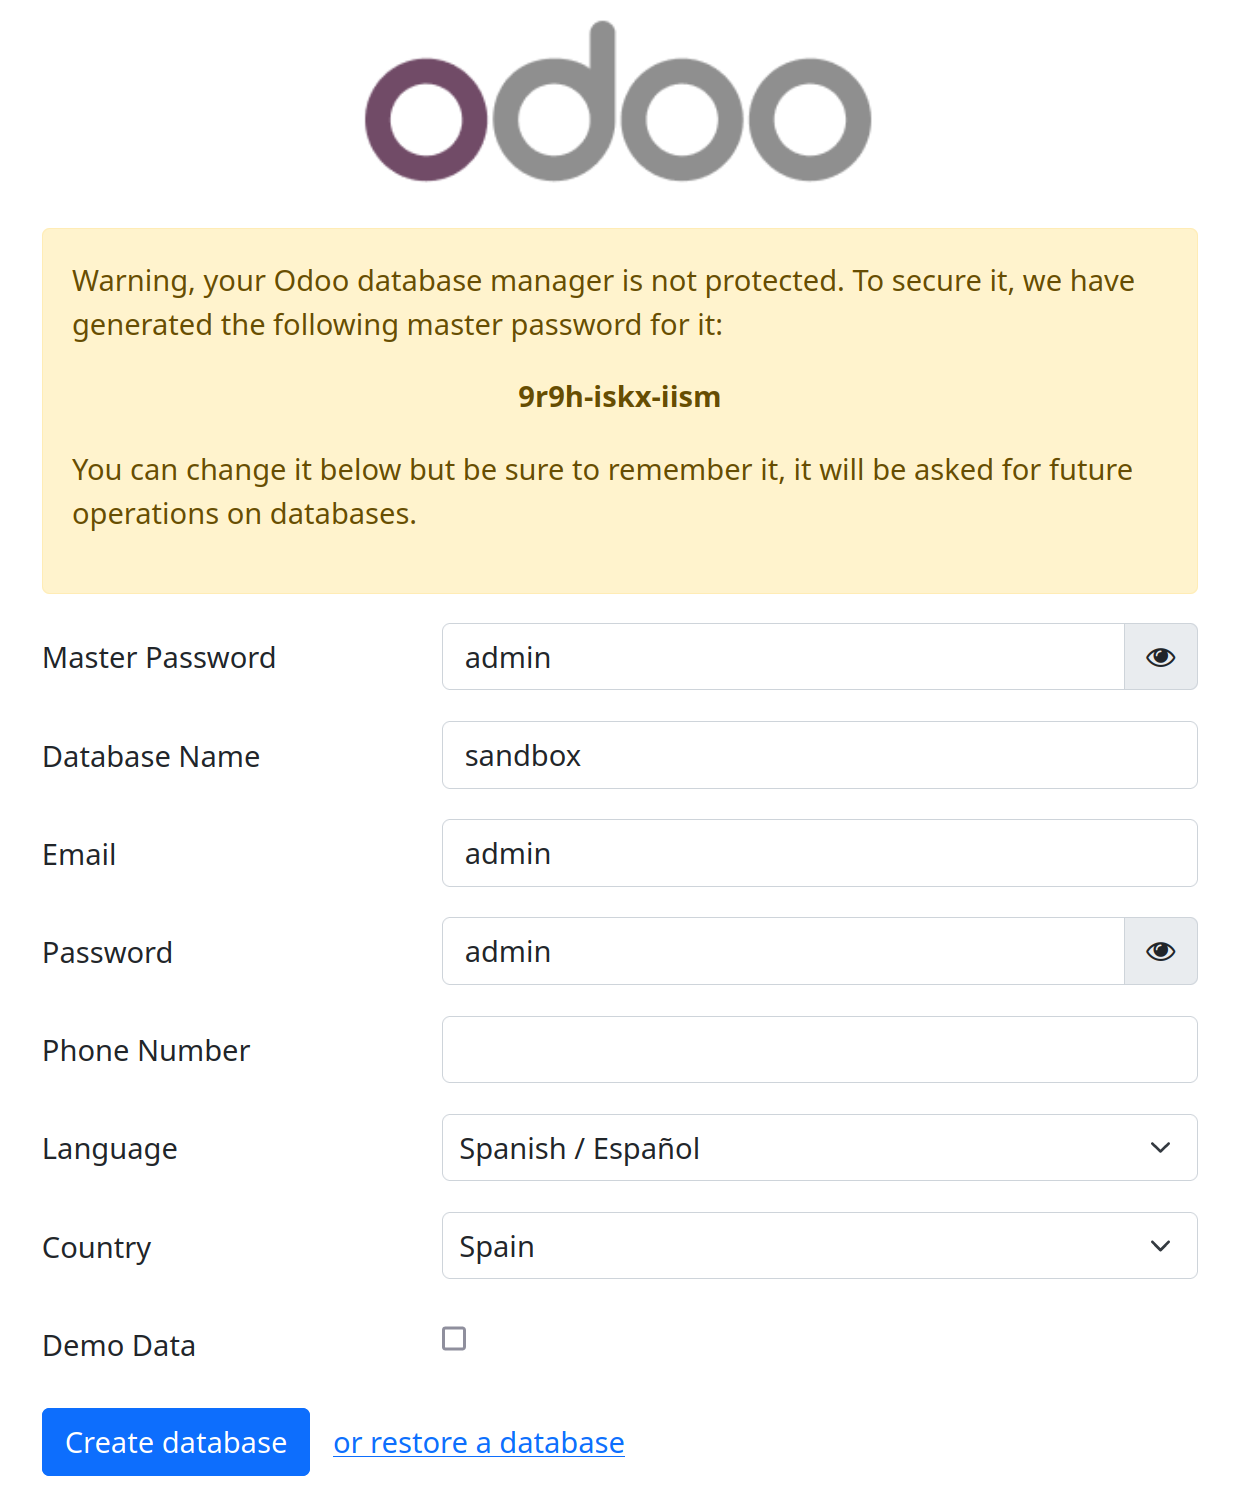
\includegraphics[width=6cm]{instalacion/signup.png}
    \caption{Proceso de registro en Odoo}
    \label{fig:signup}
\end{figure}
\paragraph{}
Por último, cuando se tenga que iniciar sesión, se tendrán que introducir las credenciales previamente definidas.

\subsubsection{Comprobación y creación de sitio web}
\paragraph{}
Con estos pasos se ha conseguido tener instalado Odoo en la máquina de forma local. Para comprobar su correcta instalación, podemos probar el módulo \textit{Blog}. Tras iniciar sesión por primera vez nos redirigirá a la ventana de \textit{Aplicaciones}, en caso contrario se ha de  navegar manualmente. Luego, se ha eliminado el filtro de \textit{Aplicaciones} de la barra de búsqueda y se ha buscado \textit{Blog}.
\paragraph{}
\paragraph{}
Se ha hecho clic en \textit{Activar} dentro de la tarjeta de Blog para instalar automáticamente los módulos relacionados con la web.
\paragraph{}
En este menú, se ha seleccionado la opción de \textit{Vamos a hacerlo}, que permite crear la web de forma sencilla en cuatro pasos. Se ha seleccionado e introducido la información que más se adecua al caso particular y se han personalizado los colores y características de la web. A continuación, se ha creado la web siguiendo la información proporcionada. En este caso, se ha creado una web de venta de coches:
\paragraph{}
\begin{figure}[h]
    \centering
    
\includegraphics[width=1\linewidth]{instalacion/web.png}
    \caption{Sitio web creado automáticamente}
    \label{fig:web}
\end{figure}
\paragraph{}
Se ha hecho clic en la opción \textit{Nuevo} en la esquina superior derecha y selecciona \textit{Entrada de blog}. Elige un blog existente o crea uno nuevo. Se ha introducido el título de la entrada de blog y pulsa \textit{Guardar}. Se mostrará la entrada de blog creada junto con un menú donde editar esta vista.
\paragraph{}
Si se hace clic en el fondo verde que engloba el título, se puede editar y añadir una imagen al fondo. Además, si se desea añadir una galería de fotos sobre el producto, en este caso un coche, se puede arrastrar la galería de imágenes desde el menú lateral derecho de edición y soltarlo en la parte de la web donde se desea ubicar.
\paragraph{}
Si se hace clic en la galería, se mostrará un menú de edición en el lateral derecho donde se puede editar y personalizar. Para añadir las imágenes que se desean mostrar, haz clic en \textit{Añadir} en la opción de imágenes dentro de la sección \textit{Galería de imágenes} del menú de edición. Luego, haz clic en \textit{Subir archivo} y selecciona las imágenes. Una vez subidas las fotos a Odoo, haz clic en cada imagen de la galería y selecciona la foto a mostrar.
\paragraph{}
Si se quiere dar acceso a la compra del producto mostrado, se añadirá un bloque llamado \textit{Llamamiento a la acción} de la misma manera que se ha hecho la galería de imágenes. Además, se puede editar cualquier texto de la web para adecuar la información a las necesidades.

\begin{figure}[h]
    \centering
    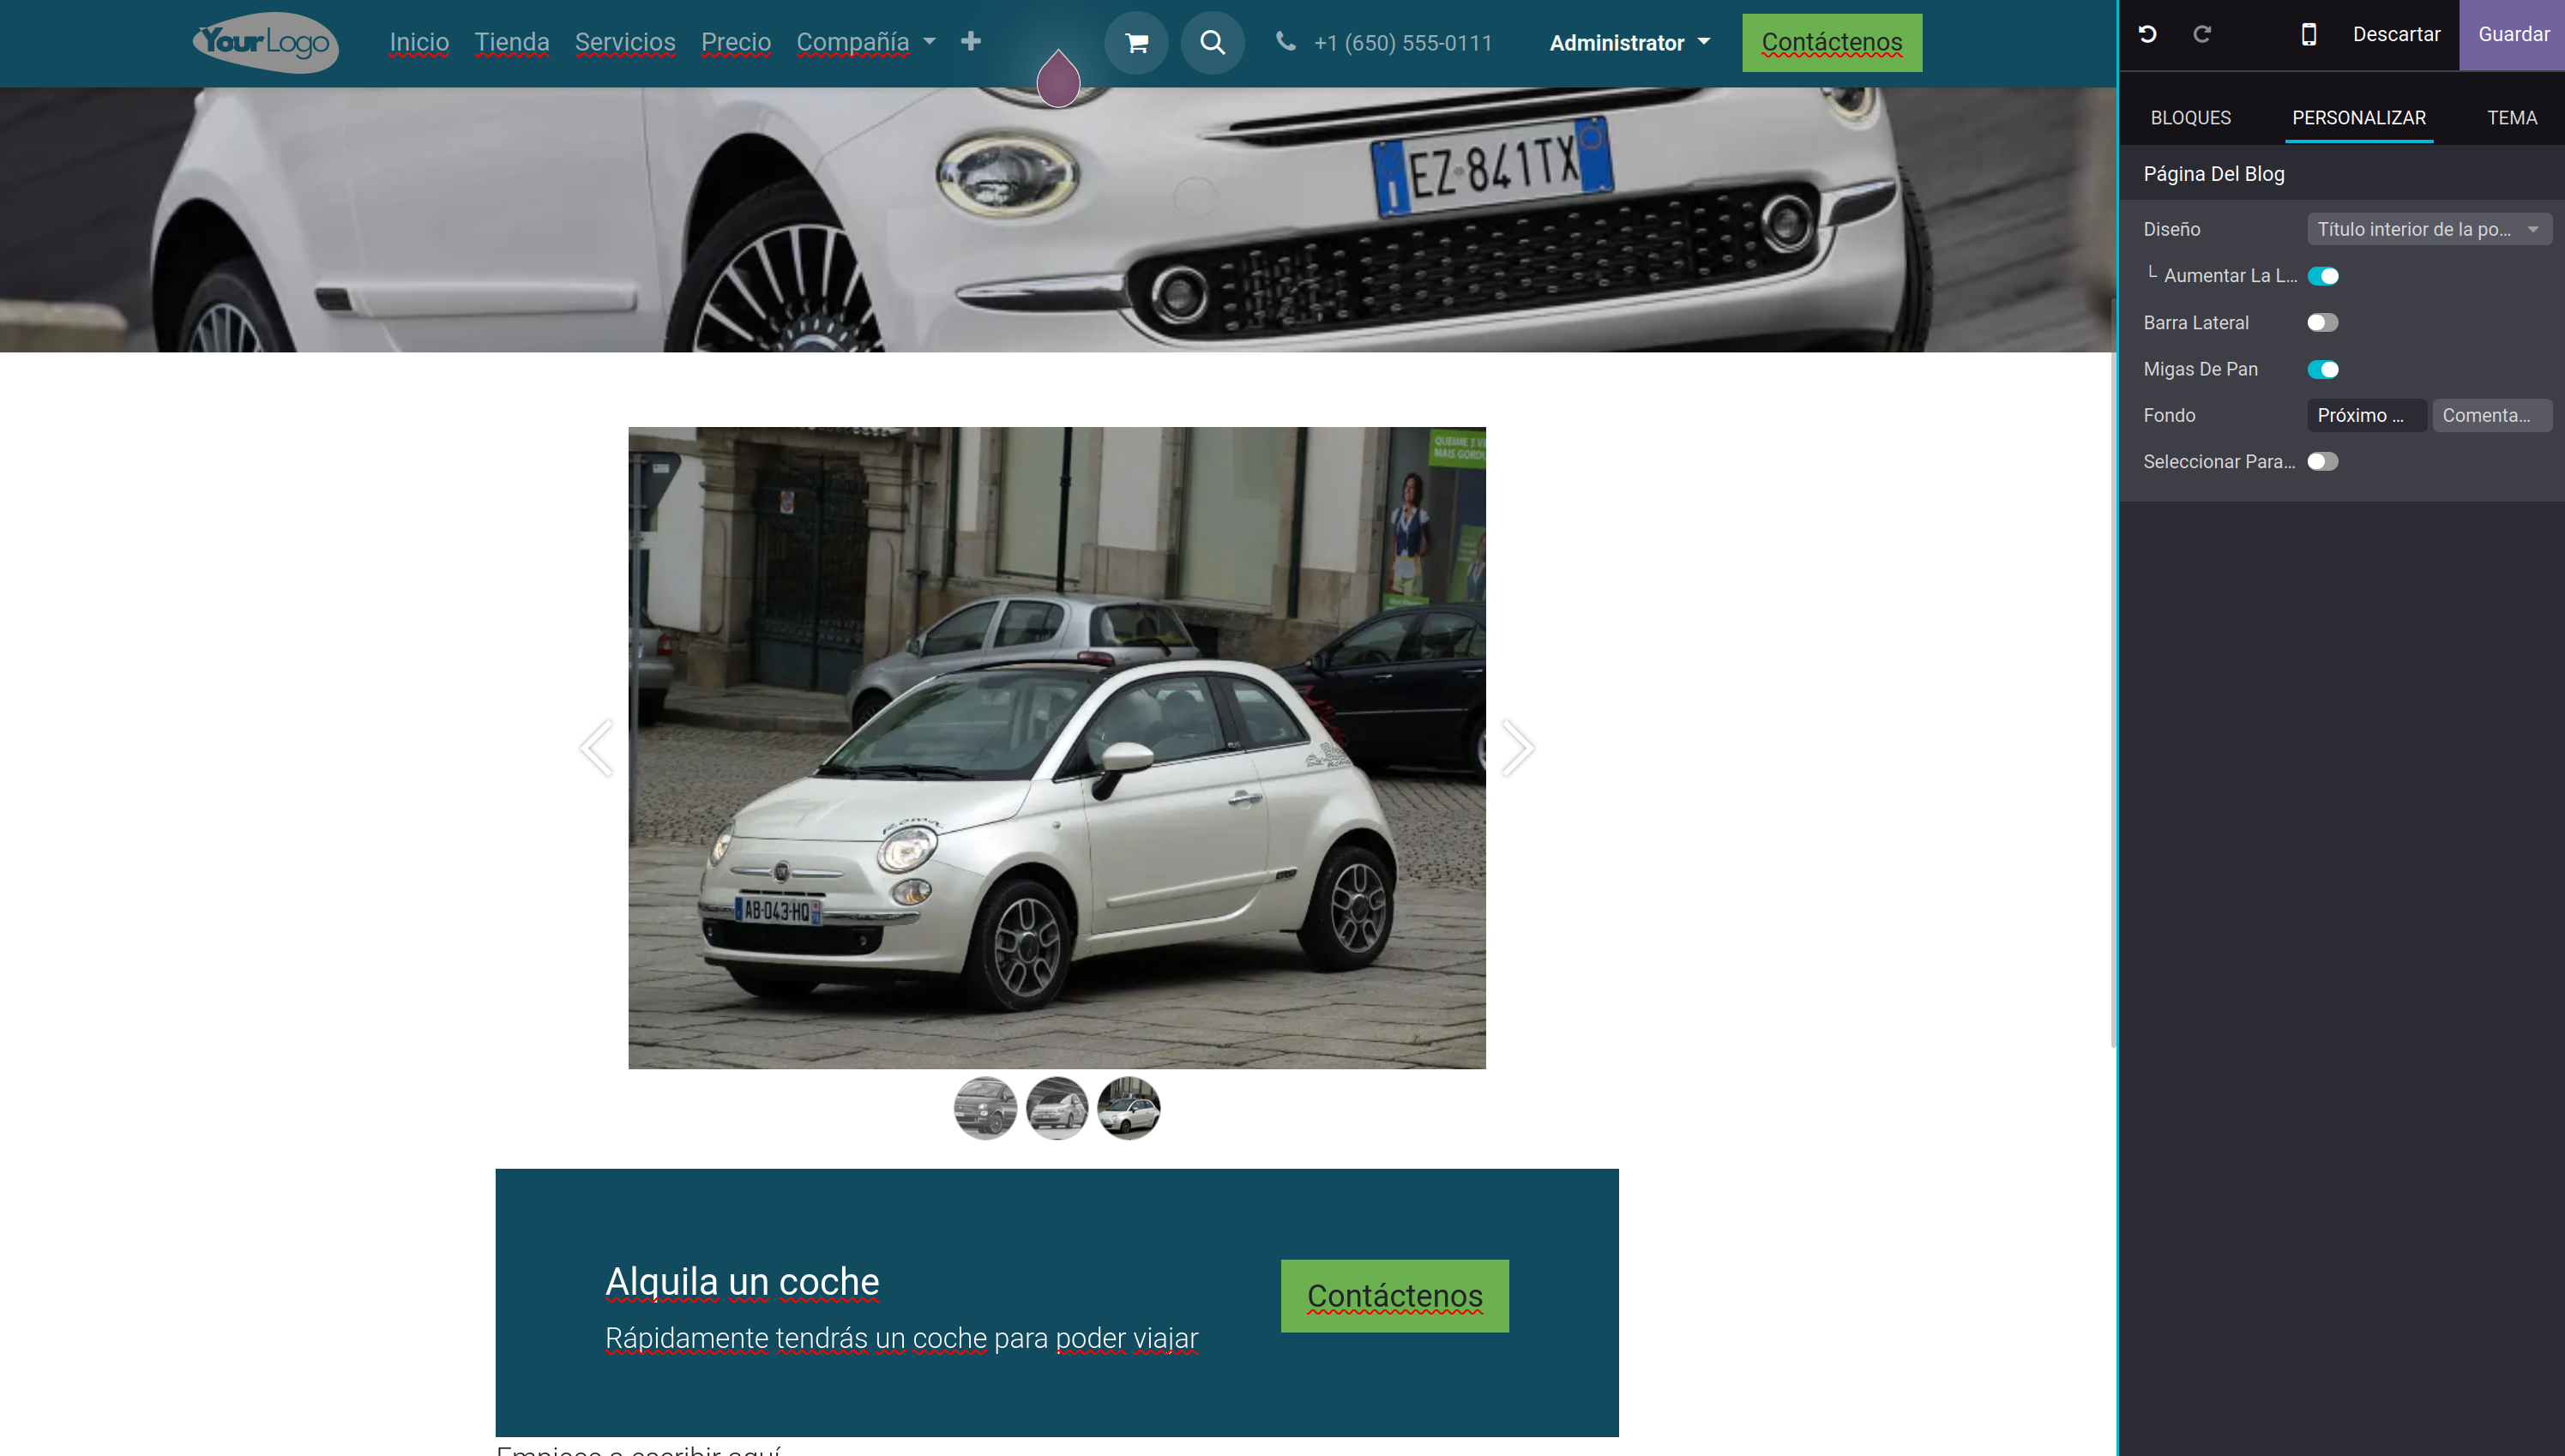
\includegraphics[width=1\linewidth]{instalacion/callToAction.png}
    \caption{Adición de un llamamiento a la acción a la entrada de blog}
    \label{fig:callToAction}
\end{figure}
\paragraph{}
Una vez que la entrada de blog esté personalizado, se ha guardado haciendo clic en el botón \textit{Guardar} en la esquina superior derecha.
\paragraph{}
Para añadir una página nueva al sitio web, se ha añadio una página. Se ha seleccionado la opción \textit{Servicios} del menú lateral izquierdo y se ha elegido la página que más se adecua a tus necesidades. En este caso, se ha creado un sitio con preguntas frecuentes, problemas comunes y sus soluciones, por lo que se ha elegido la segunda opción. Se ha introducido el título de la página, se ha activado la opción \textit{Añadir al menú} y pulsa \textit{Crear}. Edita y personaliza cada texto y foto para que se ajuste a tus necesidades. Nos hemos enfocado en el contenido importante de esta página, que son las preguntas frecuentes y los problemas comunes con sus soluciones. Para ello, se ha utilizado el bloque acordeón que ya existe en la parte inferior de la página. Para añadir nuevos temas, se ha hecho clic en el acordeón y luego en \textit{Añadir artículo} en la opción \textit{Tema} de la sección \textit{Acordeón} del menú lateral derecho. Finalmente, se ha hecho clic en \textit{Guardar} en la esquina superior. Siguiendo estos pasos, conseguimos tener instalado Odoo en nuestras máquinas locales y hemos comprobado su correcto funcionamiento desarrollando un sitio web para nuestra empresa con entradas de blog.

\subsubsection{Instalación en máquina remota}
\paragraph{}
Tener Odoo en nuestra máquina local complica el acceso desde cualquier lugar del mundo, por lo que hemos analizado la viabilidad de instalar Odoo en una máquina remota que nos permita acceder desde el navegador. Hemos investigado distintos servicios de \textit{cloud computing}; \href{https://azure.microsoft.com/en-us/}{Azure}, \href{https://aws.amazon.com}{\textit{Amazon Web Service (AWS)}} y \href{https://railway.app}{\textit{Railway.app}}. Tras analizar sus ventajas y desventajas, hemos decidido utilizar \textit{AWS}. Esta decisión se basó en su facilidad para crear una máquina, la intuición de su interfaz de consola para gestionar las máquinas y su \textit{pricing}, ya que al ser una cuenta nueva, tenemos una máquina gratuita durante un periodo de tiempo limitado; suficiente para realizar este análisis.

\paragraph{}
Lo primero que se debe hacer es crear una cuenta en \textit{AWS}. Después de rellenar nuestros datos y crear la cuenta, iniciamos sesión en la consola de \textit{AWS} y nos abrirá el menú principal como en la figura \ref{aws-home}. Seleccionamos el servicio EC2 para lanzar una instancia. Se nos redirigirá a una página donde debemos configurar la máquina que vamos a usar. En nuestro caso, hemos seleccionado un Ubuntu con la configuración predeterminada propuesta por Amazon.

\begin{figure}[h]
    \centering
    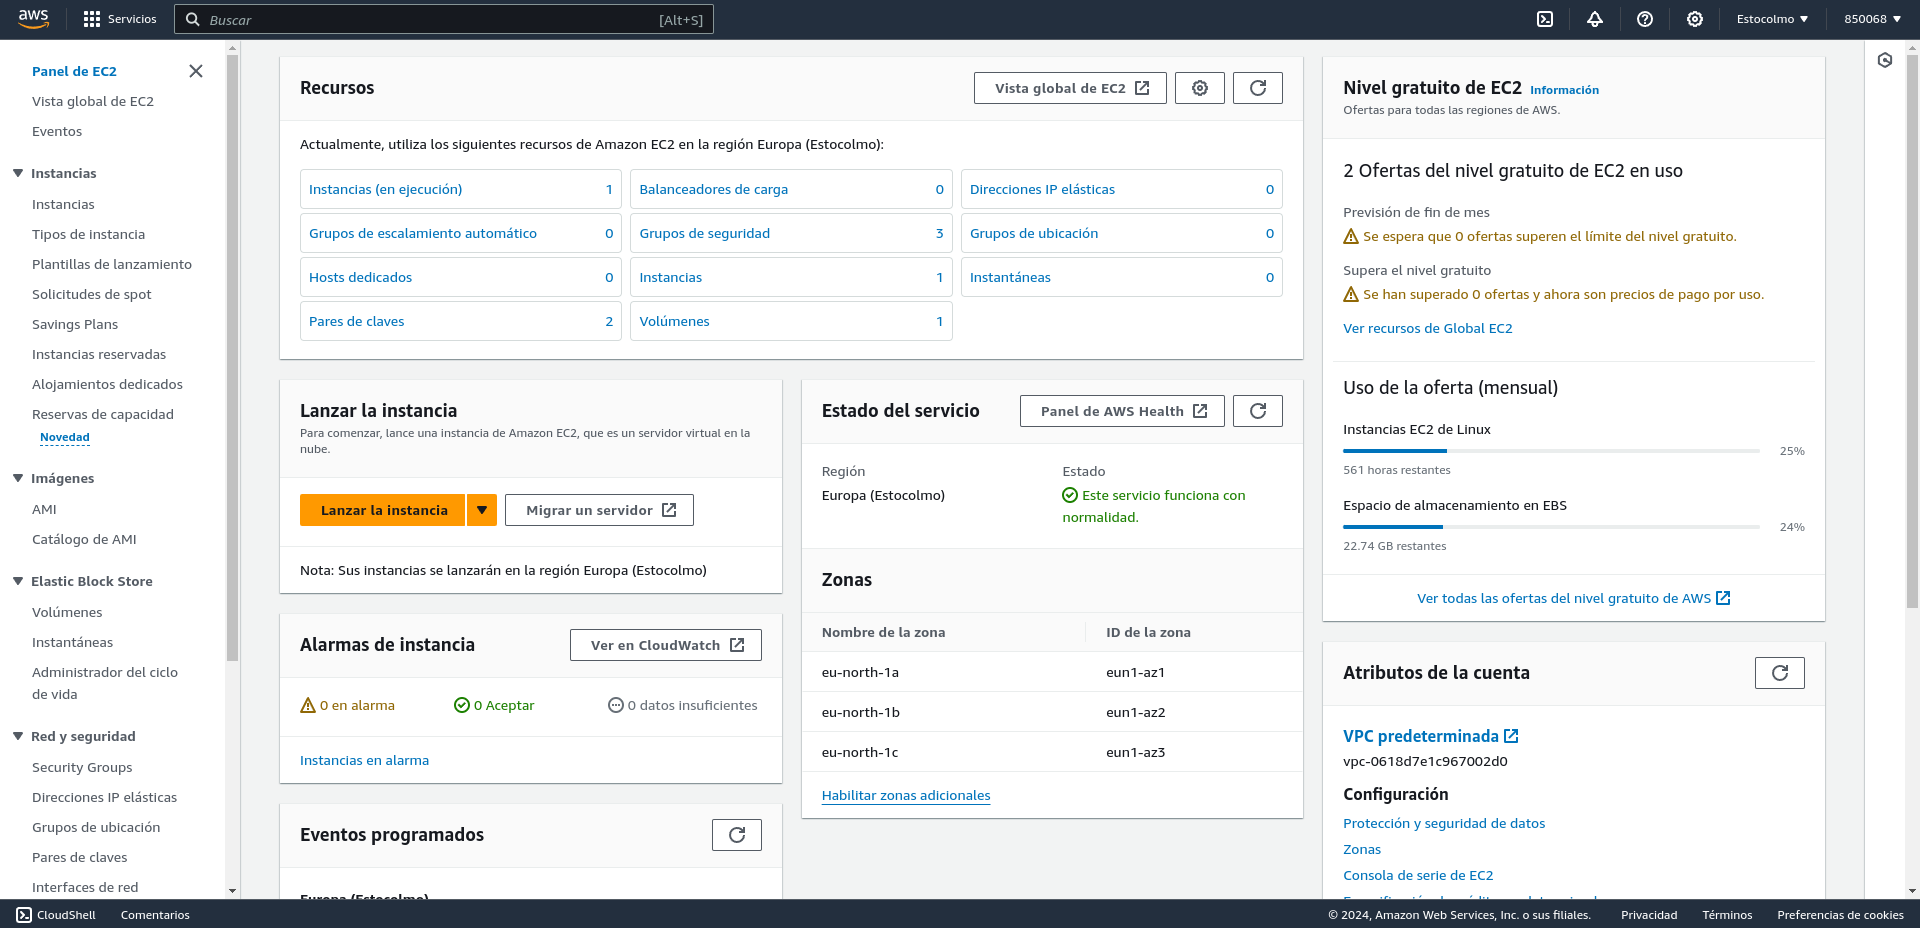
\includegraphics[width=1\linewidth]{instalacion/aws.png}
    \caption{Consola AWS}
    \label{aws-home}
\end{figure}

\paragraph{}
Una vez que se ha creado la instancia, se deben crear un par de claves para acceder a la máquina. Seleccionamos en el menú \textit{Red y seguridad} \textgreater{} \textit{Pares de claves} \textgreater{} \textit{Crear par de claves}. Introducimos el nombre que deseamos y creamos el par de claves. Se descargará la clave recién creada.

\paragraph{}
Por último, debemos configurar las reglas de seguridad para permitir el tráfico HTTPS en el puerto 8069. Para ello, seleccionamos en el panel lateral \textit{Grupos de seguridad} \textgreater{} \textit{Crear grupo de seguridad}. Introducimos el nombre que deseamos y agregamos una regla de entrada: debe ser TCP personalizado con intervalo de puertos de 8069. Guardamos las reglas y ya podremos desplegar el contenedor con Odoo en nuestra máquina EC2.

\paragraph{}
Para realizar la conexión a nuestra máquina, abrimos una terminal e introducimos el siguiente comando en un ordenador MacOS o Linux:

\begin{lstlisting}[frame=single, basicstyle=\small]
ssh -i "ruta/a/tu/clave.pem" usuario@direccion-IP-de-la-instancia
\end{lstlisting}

\paragraph{}
Donde se deben sustituir los campos por los que correspondan. Una vez que se ha realizado la conexión SSH con la máquina, se deben seguir los mismos pasos explicados previamente para lanzar Odoo en la sección de instalación local.

\subsection{Resultados y análisis}
\paragraph{}
Una vez completada la instalación de Odoo tanto en una máquina local como en una máquina remota, se realizaron pruebas de funcionamiento para evaluar la efectividad de ambos métodos.

\subsubsection{Instalación local}
\paragraph{}
La instalación de Odoo localmente permitió verificar que el sistema se ejecuta de manera eficiente y rápida, brindando acceso a todas las funcionalidades del ERP sin mayores problemas. Además, el uso de Docker facilitó la gestión de las dependencias y la configuración, reduciendo el riesgo de errores de compatibilidad.
\paragraph{}
Sin embargo, operar localmente limita el acceso a Odoo a la máquina específica donde está instalado, lo que puede dificultar la colaboración remota o el acceso desde distintos dispositivos y ubicaciones.

\subsubsection{Instalación en máquina remota}
\paragraph{}
La instalación de Odoo en una máquina remota, utilizando los servicios de \textit{AWS}, permitió acceder al sistema desde cualquier lugar con conexión a internet. Esta flexibilidad facilita la colaboración entre diferentes equipos y departamentos, al permitir el acceso simultáneo y remoto a Odoo.
\paragraph{}
Durante las pruebas, se comprobó que la instalación remota ofrece un rendimiento similar al local, con la ventaja adicional de la escalabilidad que ofrece la infraestructura de \textit{AWS}. Esta opción es especialmente útil para nuestra empresa, dadas las necesidades de acceso distribuido y el posible alto volumen de usuarios.

\subsubsection{Comparación}
\paragraph{}
En resumen, aunque la instalación local ofrece mayor control sobre el sistema, la instalación remota brinda flexibilidad y escalabilidad para el acceso desde cualquier ubicación. Dependiendo de las necesidades específicas de la empresa, ambas opciones pueden ser adecuadas, aunque se recomienda la instalación remota debido a la necesidad de acceso desde múltiples ubicaciones y una infraestructura escalable.

\subsection{Conclusiones}
\paragraph{}
En base a los resultados obtenidos durante la instalación y prueba de Odoo, se pueden extraer las siguientes conclusiones:

\begin{itemize}
    \item La instalación de Odoo localmente es adecuada para entornos de desarrollo o pruebas, donde se requiere acceso rápido y control directo sobre el sistema.
    \item La instalación remota, utilizando servicios de \textit{cloud computing} como \textit{AWS}, ofrece una solución escalable y flexible que permite el acceso desde cualquier ubicación con conexión a internet.
    \item La instalación remota es especialmente recomendable para entornos empresariales que requieran acceso distribuido y colaboración entre diferentes equipos y departamentos.
    \item Se recomienda continuar utilizando la instalación remota para aprovechar la escalabilidad y flexibilidad que ofrece la infraestructura en la nube.
\end{itemize}
\paragraph{}
En general, la instalación de Odoo, tanto local como remota, demuestra ser una solución efectiva para la gestión empresarial, permitiendo optimizar y agilizar los procesos internos de la empresa.

\newpage

\section{Configuración funcional - Organización de la empresa}
\subsection{Autoevaluación}
En esta sección se han cumplido los objetivos correspondientes al 10.
\subsection{Introducción}
Este módulo se enfoca en la gestión y la organización de la empresa que Odoo nos permite realizar. Se va a describir como se ha creado una nueva compañía, la distribución de usuarios entre las entidades y la organización estructural de la empresa. Además, de explora la internacionalización en Odoo, donde se prueba el soporte multilingüe y el manejo de distintas monedas .
\subsection{Metodología}
\paragraph{}
En cuanto a la creación de una nueva compañía, el proceso ha comenzado accediendo al menú de configuración dentro de las opciones generales. Luego, se ha hecho clic en el enlace \textit{Administrar compañías} para iniciar el proceso de creación de la empresa. Posteriormente, se ha completado el formulario correspondiente. Después, se ha navegado hasta el menú de \textit{Ramas de la compañía} para gestionar las sucursales de la compañía matriz recién creada, agregando dos nuevas: CochesMA.UK y CochesMA.US
\paragraph{}
Además, se ha procedido a gestionar los usuarios para las compañías creadas, tanto la matriz como las sucursales. Para ello, en las opciones generales de los ajustes de Odoo, se ha pulsado en \textit{Administrar usuarios}. Desde este menú se han creado 9 usuarios, seleccionando \textit{Nuevo} y completando el formulario correspondiente. Es importante destacar que se puede seleccionar a qué compañías tiene acceso cada usuario. Además, se puede cambiar el idioma para el usuario desde el menú de preferencias. En caso de que el idioma deseado no aparezca, se ha pulsado en el icono del mundo para buscarlo.
\paragraph{}
Por otro lado, Odoo ofrece herramientas de internacionalización, incluyendo soporte multilingüe. Para configurarlo, se ha accedido a las opciones generales de los ajustes, donde se ha seleccionado \textit{Añadir idiomas} y se han escogido los idiomas deseados. También es posible establecer varias monedas dentro de la compañía. Para ello, se ha seleccionado la compañía matriz en la opción de \textit{Administración de compañías} dentro de las opciones generales, y en la sección de \textit{Moneda} se han activado las monedas que se desean utilizar tanto en la matriz como en las sucursales. Finalmente, se ha seleccionado la moneda que se utilizará como predeterminada.
\subsection{Resultados y análisis}
Se ha llevado a cabo el proceso de creación de una compañía matriz llamada CochesMA la cual tiene dos compañías rama, una en Reino Unido llamada CochesMA.UK y otra en Estados Unidos llamada CochesMA.US.
\begin{figure}[h]
    \centering
    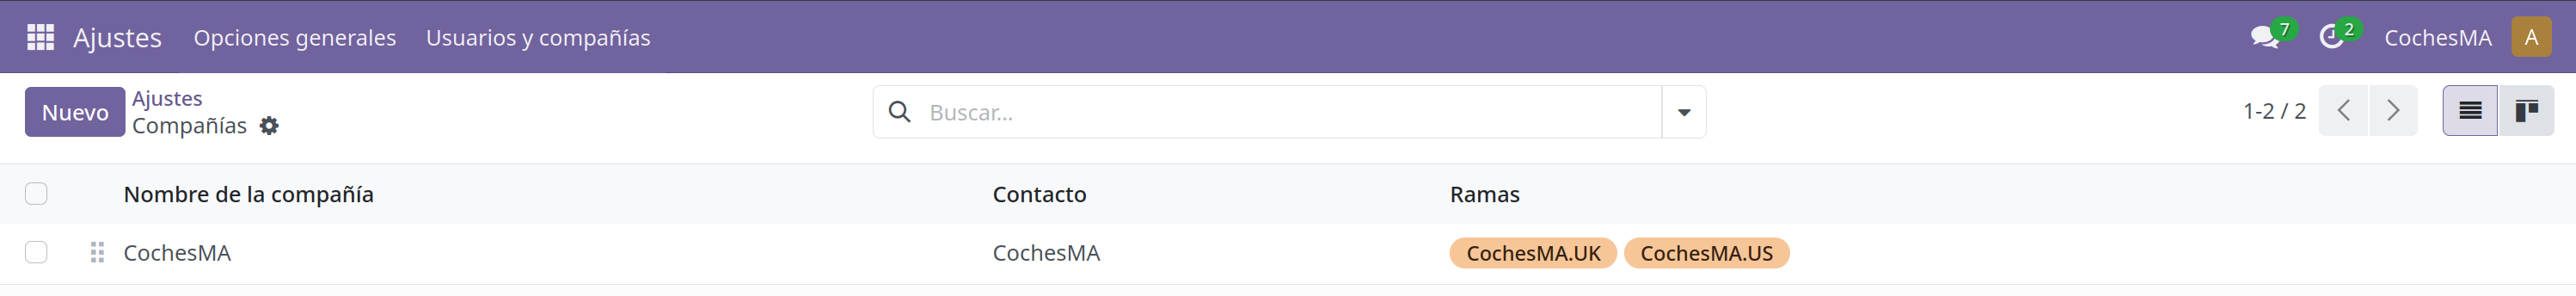
\includegraphics[width=\linewidth]{fotosConfiguración/estructuraEmpresarial.png}
    \caption{Compañía matriz con sus dos compañías rama}
    \label{fig:enter-label}
\end{figure}
\begin{figure}[h]
    \centering
    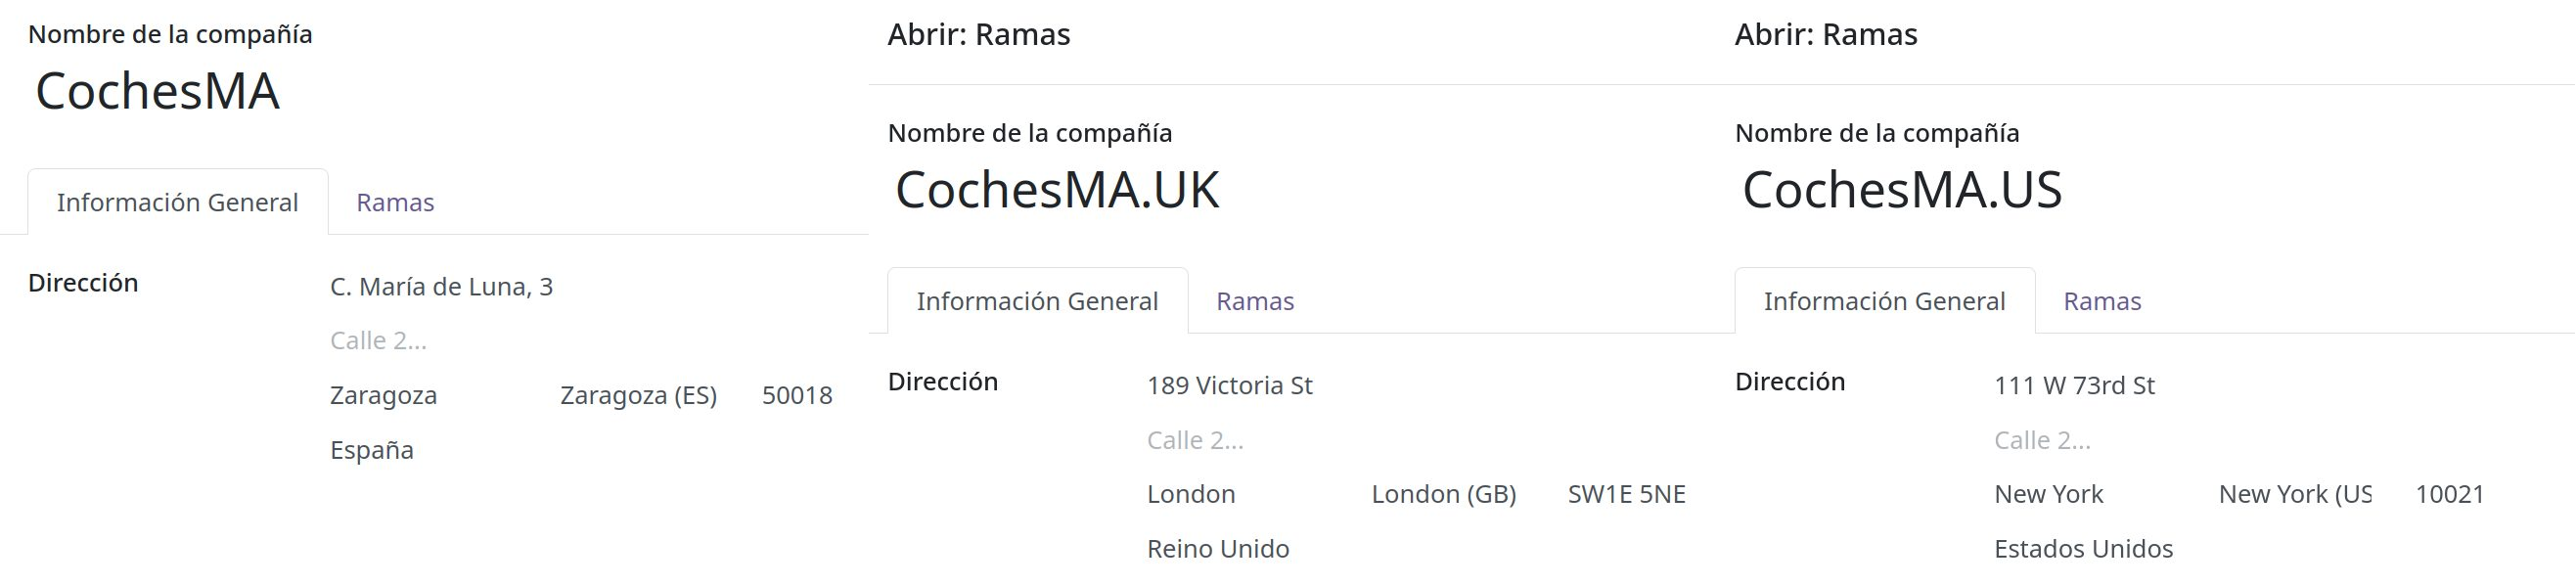
\includegraphics[width=\linewidth]{fotosConfiguración/ubicaciones.jpg}
    \caption{Ubicaciones de las compañias}
    \label{fig:enter-label}
\end{figure}
Se han creado 9 usuarios. John, James, Marcus, Mark, Sheila y Tom hablan ingles y Juan, Maria y Pedro hablan español. John, James y Pedro pertenecen a la compañía matriz. Juan, Marcus y Sheila pertenecen a la rama de Estados Unidos. Maria, Mark y Tom pertenecen a la rama de Reino Unido.
Además, se han añadido los idiomas de los usuarios a Odoo y se ha establecido la siguiente la moneda principal el Euro, pero se ha permitido el uso de la Libra esterlina para CochesMA.UK y el Dolar estadounidense para CochesMA.US. 
\begin{figure}[h]
    \centering
    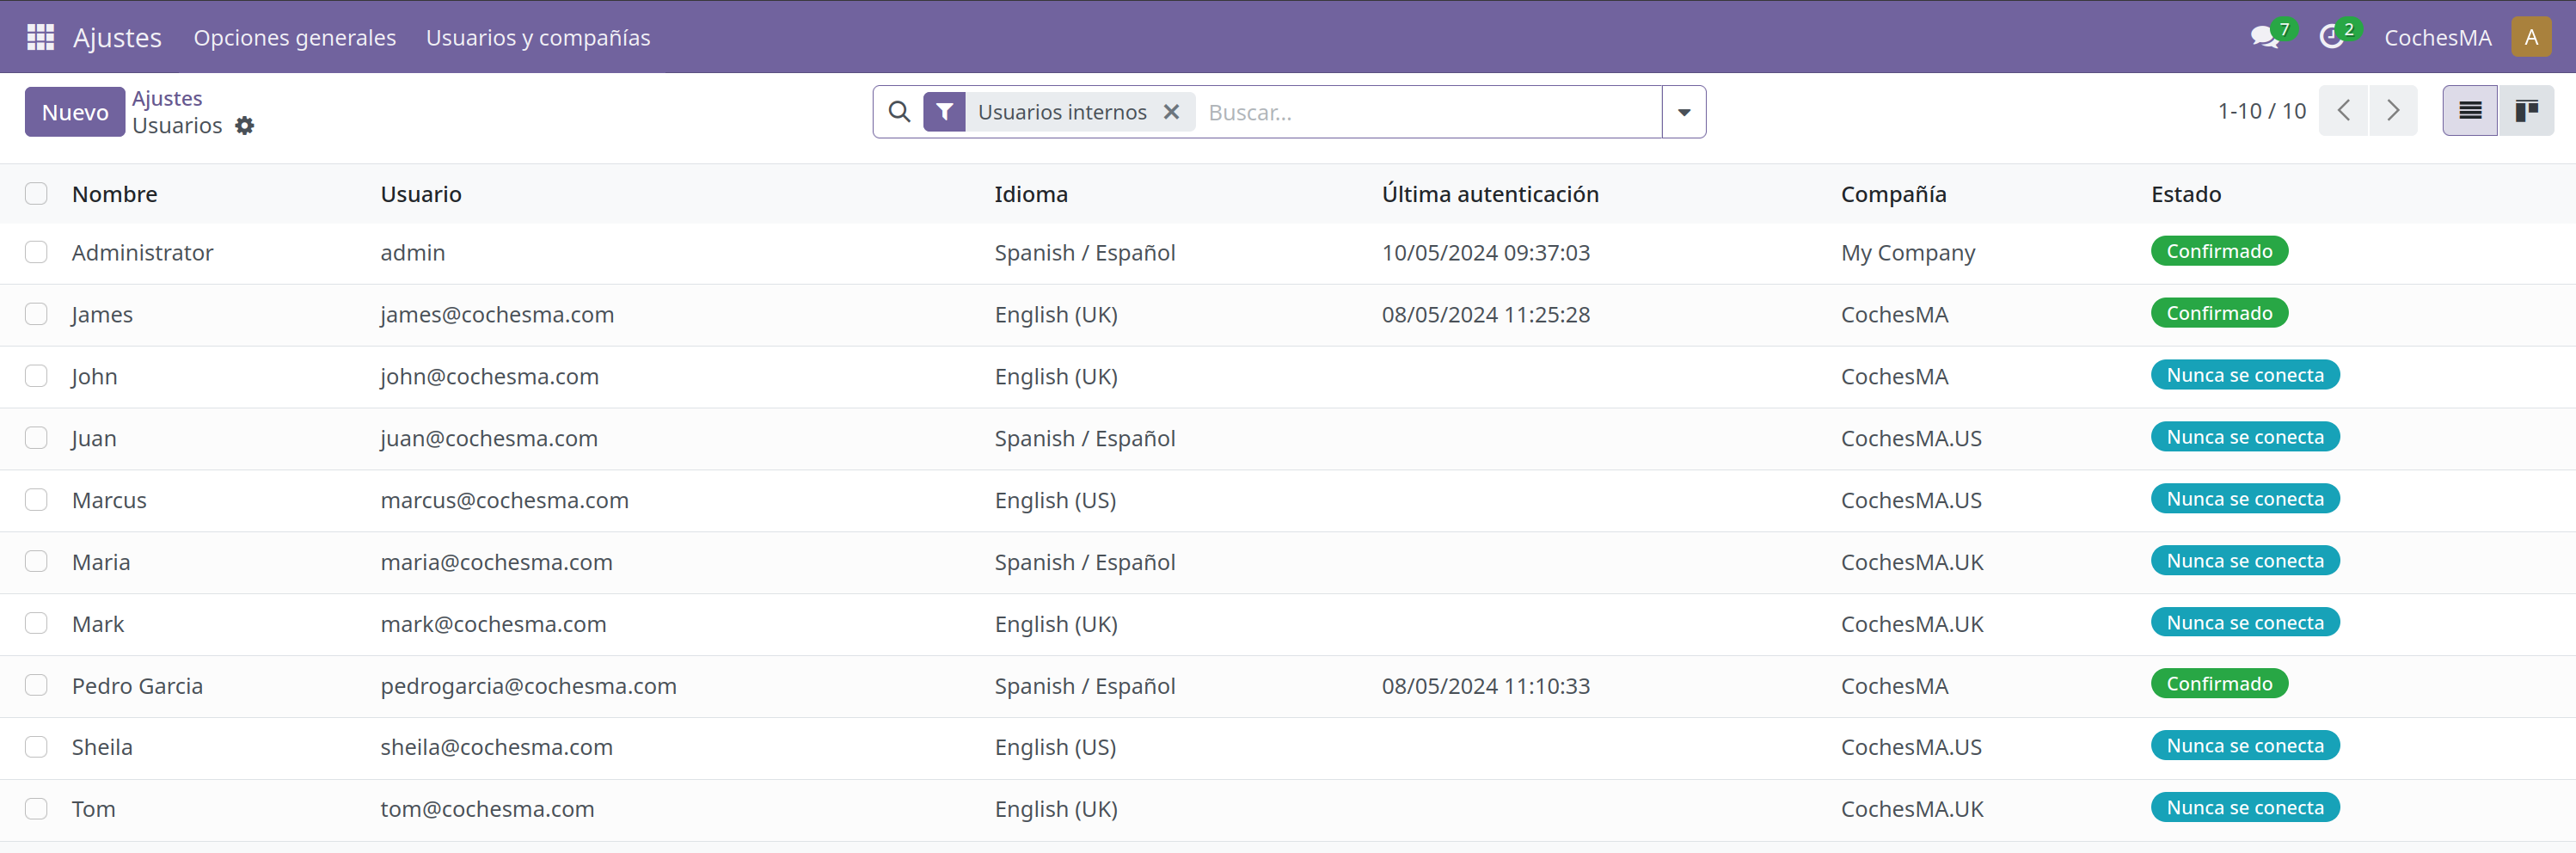
\includegraphics[width=\linewidth]{fotosConfiguración/usuarios.png}
    \caption{Usuarios creados con su idioma y compañía}
    \label{fig:enter-label}
\end{figure}

\begin{figure}[h]
    \centering
    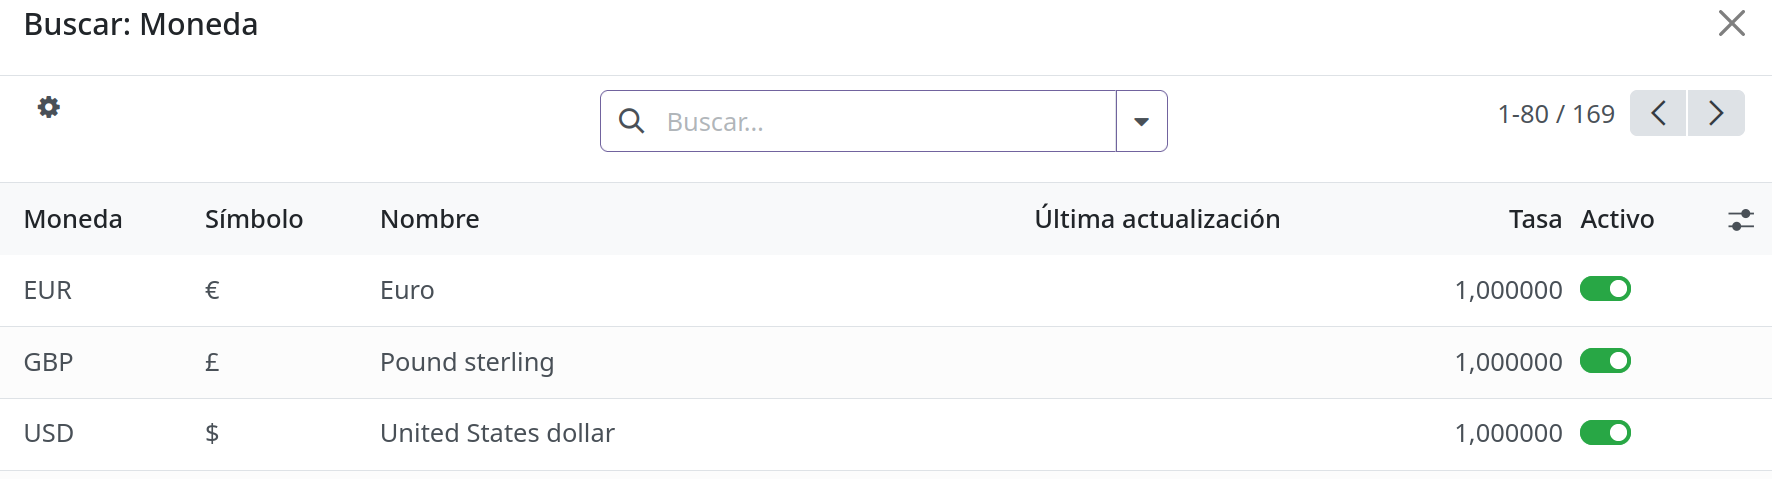
\includegraphics[width=\linewidth]{fotosConfiguración/divisas.png}
    \caption{Divisas de las compañías}
    \label{fig:enter-label}
\end{figure}
\subsection{Conclusiones}
La capacidad de Odoo para gestionar múltiples compañías se demuestra en la capacidad que tiene para adaptarse a estructuras empresariales con empresas matrices y ramas.
En cuanto al proceso de creación de usuarios en Odoo es sencillo y permite especificar detalles como la compañía a la que pertenecen, su acceso a los módulos y su idioma preferido, agilizando así el proceso de integración. La posibilidad de añadir nuevos idiomas al sistema de forma sencilla mejora la experiencia del usuario y facilita la comunicación en entornos internacionales.
Sin embargo, es importante tener en cuenta que, aunque la creación de una nueva compañía y la gestión de sus ramas se realiza de manera intuitiva, la gestión de múltiples monedas puede resultar un poco más oculta. Para activar las monedas, es necesario pulsar en \textit{Buscar más}, y existen ciertas restricciones, como la obligación de que las empresas filiales tengan la misma moneda que la matriz.
En general, son aspectos básicos del sistema que son fáciles de configurar aunque tienen gran importancia ya que son la base sobre la que se construirán las personalizaciones de los siguientes módulos.
\newpage
\section{Configuración funcional - Imagen corporativa}
\subsection{Autoevaluación}
En esta sección se han cumplido los objetivos correspondientes al 10.
\subsection{Introducción}
Este apartado se enfoca en mejorar la presencia digital de la empresa. Inicia con la activación del sistema multilingüe en la web, para posibilitar un alcance global. También, se aborda la personalización de la página web, integrando la información de la empresa y el logo y ajustando el tema y los colores para alinearla con la imagen de la empresa. Además, se realizan optimizaciones SEO para mejorar la visibilidad de la web en los motores de búsqueda y la implementación de SSL para garantizar la seguridad.
\subsection{Metodología}
\paragraph{}
Para probar el sistema multilingüe de la web hay que asegurase que los idiomas deseados están en el apartado de sitio web de la configuración y si no añadirlo desde ahí, cabe destacar que sólo dejará añadir idiomas que tengan los usuarios de la compañía. Una vez realizado este paso, el usuario podrá cambiar el idioma en la web desde la esquina superior izquierda o en el pie de página. 
\paragraph{}
Además, se ha llevado a cabo la personalización de la página web para incluir la información de la empresa. Para ello, se ha accedido al modo de edición navegando a la página web y seleccionando el modo de edición. Se ha ido a la página \textit{Contáctenos}, se ha editado haciendo haciendo doble clic en el bloque de la geolocalización y se ha introducido la información de la dirección, el correo electrónico y el teléfono, al igual que en el pie de página que es común en muchas páginas de la web. Además, en la pantalla \textit{Home} de la página web se ha editado el bloque de la misión y el bloque de Acerca de en el pie de página de la misma manera. 
\paragraph{}
Por otro lado, también se puede cambiar tanto los colores como el tema de la web. Para ello, se debe estar en el modo edición en la web y seleccionar el menú \textit{Tema} en la barra lateral derecha. A continuación, se puede cambiar los colores tanto principales como secundarios del tema, sustituyendo los colores por otros. Si se quiere cambiar de tema, se ha hecho clic en \textit{Cambiar tema} y se ha seleccionado el nuevo tema entre los disponibles. También, se ha añadido el logo a la página web haciendo clic en el logo predeterminado. Se ha desplegado la barra lateral derecha, se ha hecho clic en \textit{Reemplazar} y se ha seleccionado el nuevo logo. En los ajustes del sitio web se ha añadido el logo en la opción de \textit{Favicon} para que también se muestre el logo en la parte superior de la pestaña en el buscador. 
\paragraph{}
Para mejorar el ranking de búsqueda con Google se han utilizado las herramientas SEO. En este menú se ha editado el título y la descripción y se ha añadido el logo para que aparezca desde el buscador. También, incluye la posibilidad de utilizar la herramienta de palabras clave, se han añadido un conjunto de palabras en la web para que cuando los usuarios busquen estas palabras aparezca nuestra web.

\paragraph{}
Una vez que hemos realizado la web hemos configurado la web de nuestra empresa en un dominio propio con acceso seguro SSL. Esta paso es esencial a la hora de determinar si este ERP es adecuado para nuestra empresa. Ya que es una funcionalidad que se va a necesitar de cara a permitir el acceso a nuestros clientes y usuarios desde cualquier navegador de forma segura. Esta configuración se ha realizado de forma local para realizar el análisis. La máquina utilizada para realizar las pruebas es un MacBook Pro de 2018 con un procesador Intel i5. El equipo a determinado que la mejor forma de montar un servidor SSL localmente es utilizando \textit{Nginx} y Docker. Se ha planteado utilizar una máquina Ubuntu y seguir los pasos descritos en: \href{https://www.digitalocean.com/community/tutorials/how-to-create-a-self-signed-ssl-certificate-for-nginx-in-ubuntu-20-04-1}{How To Create a Self-Signed SSL Certificate for Nginx in Ubuntu 20.04}. Sin embargo, esta alternativa no era la mejor opción para nuestro objetivo y situación, ya que al tener Odoo desplegado en un contenedor Docker. Y esto nos permite modificar nuestro \textit{docker-compose.yml} añadiendo el servicio de Nginx, el cual nos proporciona el certificado SSL. 

\paragraph{}
Los pasos que hemos llevado a cabo para implementar un servidor SSL local en Odoo utilizando Docker Compose y Nginx han sido:\\
Lo primero que hemos realizado es generar un certificado SSL utilizando OpenSSL, el cual nos genera un par de claves públicas y privada, y un certificado autofirmado válido por un año. Para ello hemos abierto nuestra terminal y ejecutado el siguiente comando:

 \begin{lstlisting}[frame=single, basicstyle=\small]
openssl req -x509 -nodes -days 365 -newkey rsa:2048
-keyout localhost.key -out localhost.crt
\end{lstlisting}
\paragraph{}
Al ejecutarlo deberemos rellenar nuestro país, región, ciudad, nombre de la organización, nombre del departamento, nombre del dominio y un correo electrónico. Este par de claves las hemos almacenado en un directorio llamado \textit{certificados}. A continuación hemos modificado el fichero \textit{docker-compose.yml} que creamos para la instalación, obteniendo este nuevo fichero: 
\begin{lstlisting}[frame=single, basicstyle=\small]
version: "3.1"
services:
  odoo:
    image: odoo:17.0
    depends_on:
      - db
    ports:
      - "8069:8069"
    volumes:
      - odoo-web-data:/var/lib/odoo
    environment:
      - HOST=db
      - USER=odoo
      - PASSWORD=myodoo

  db:
    image: postgres:13
    environment:
      - POSTGRES_DB=postgres
      - POSTGRES_PASSWORD=myodoo
      - POSTGRES_USER=odoo
      - PGDATA=/var/lib/postgresql/data/pgdata
    volumes:
      - odoo-db-data:/var/lib/postgresql/data/pgdata

  nginx:
    image: nginx:latest
    ports:
      - "443:443"
    volumes:
      - ./certificados:/certificados:ro
      - ./nginx.conf:/etc/nginx/nginx.conf:ro
    depends_on:
      - odoo

volumes:
  odoo-web-data:
  odoo-db-data:
\end{lstlisting}

\paragraph{}
Además de este fichero debemos crear un llamado \textit{nginx.conf} en el cual definiremos la configuración básica de Nginx para SSL. Una vez que tenemos ambos ficheros correctamente configurados podemos iniciar el contenedor desde la terminal, ejecutando en el directorio correcto el comando:
 \begin{lstlisting}[frame=single, basicstyle=\small]
docker-compose up -d
\end{lstlisting}
\paragraph{}
Por último, abrimos nuestro navegador y buscamos https://localhost. Si hemos realizado todos los pasos correctamente nos tendrá que aparecer el siguiente mensaje: 
\begin{figure}[h]
    \centering
    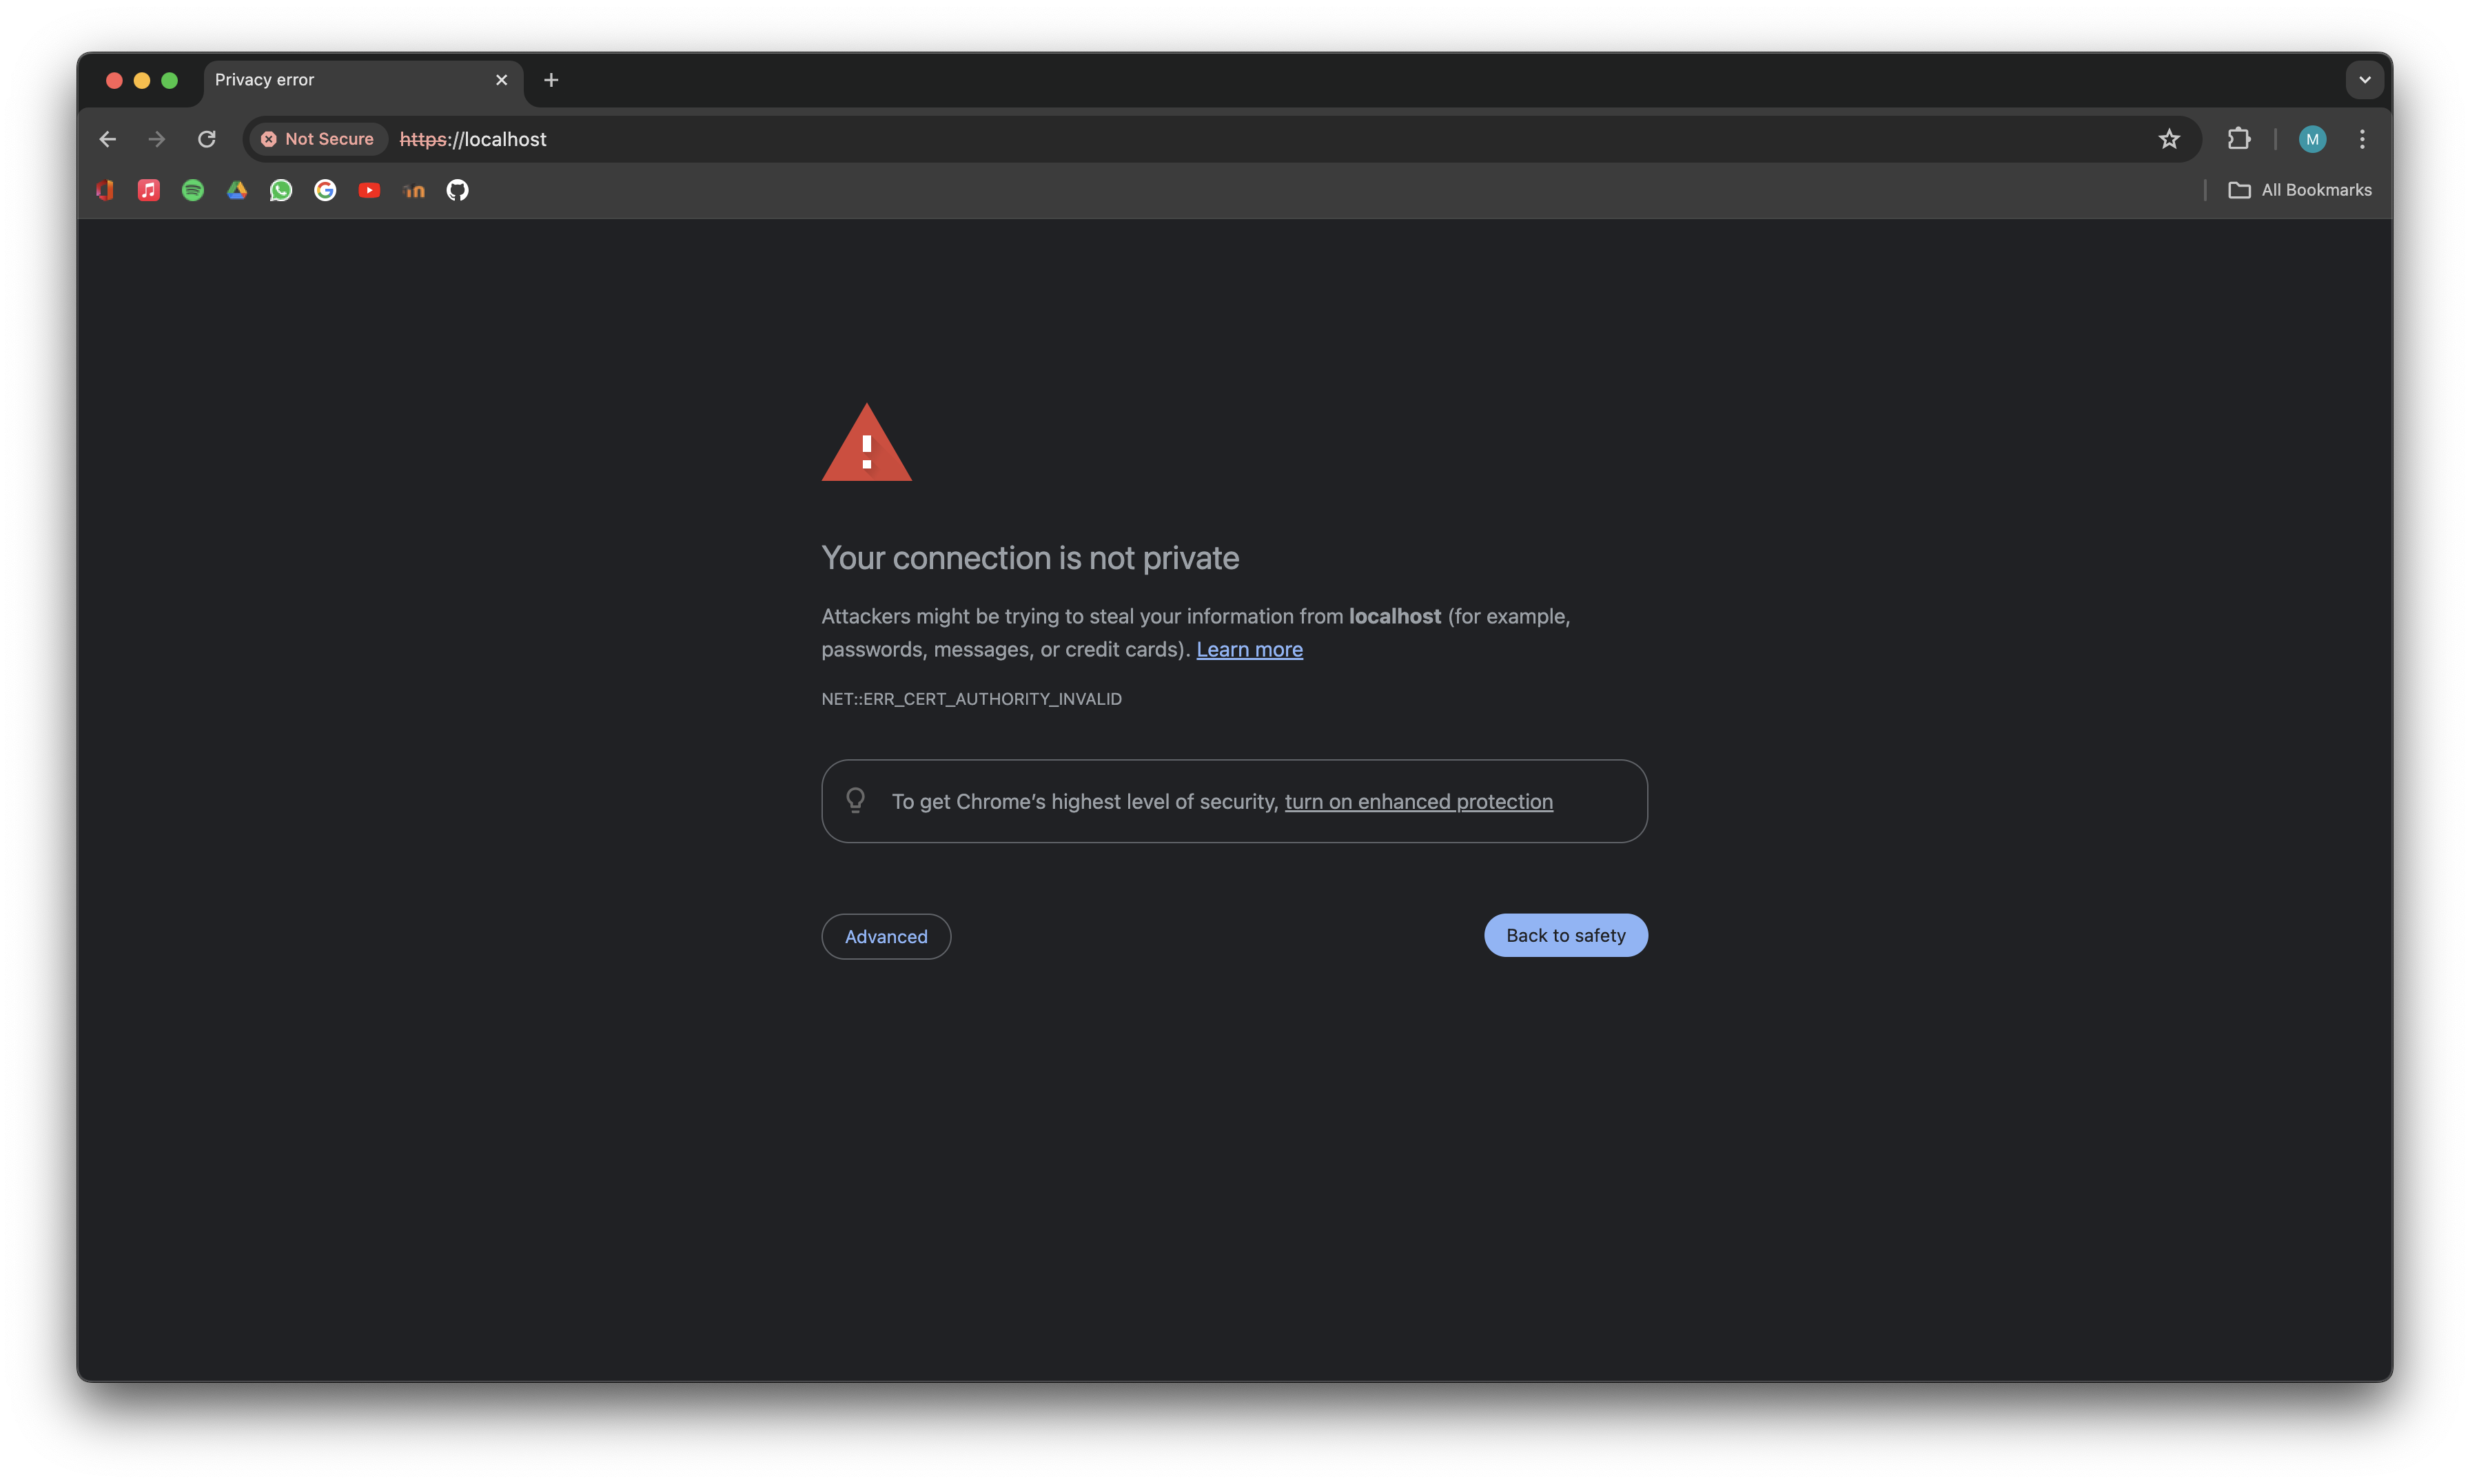
\includegraphics[width=1\linewidth]{conNotPrivate.png}
    \caption{Mensaje de conexión privada}
\end{figure}
\paragraph{}
Este mensaje es normal que nos aparezca ya que nuestro certificado no es validado por una entidad externa, ya que nosotros hemos generado un certificado auto firmado el cual simula una conexión segura HTTPS sin ningún coste adicional. Por lo tanto si pulsamos en \textit{Advanced} y luego en ir a la página se nos abrirá nuestra web con el certificado SSL.

\subsection{Resultados y análisis}
En primer lugar, se ha configurado la página web para que se pueda mostrar en 3 idiomas: Español, Inglés(UK) e Inglés(US), ya que son los 3 idiomas que se hablan donde se ubican las compañías. 
\newpage
\begin{figure}[h]
    \centering
    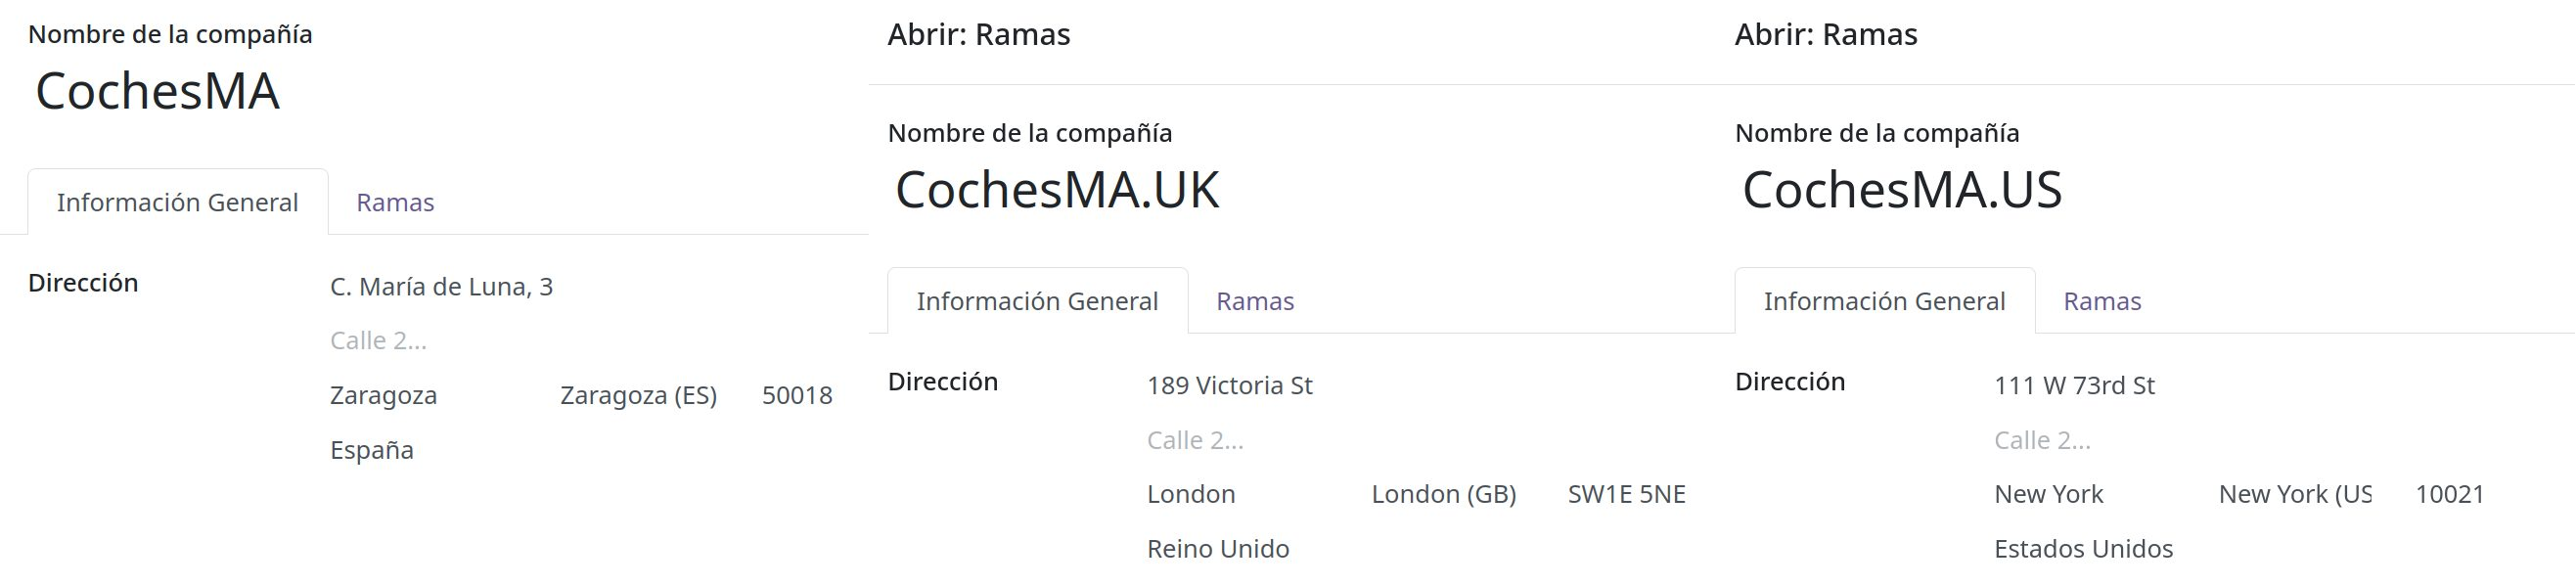
\includegraphics[width=1\linewidth]{fotosConfiguración/ubicaciones.jpg}
    \caption{Ubicación de las empresas}
    \label{fig:enter-label}
\end{figure}
Se ha personalizado la web para que contenga el logo, el nombre, la misión, el correo electrónico, la localización y el número de teléfono y se ha cambiado los colores a blanco y a azul.
\begin{figure}[h]
    \centering
    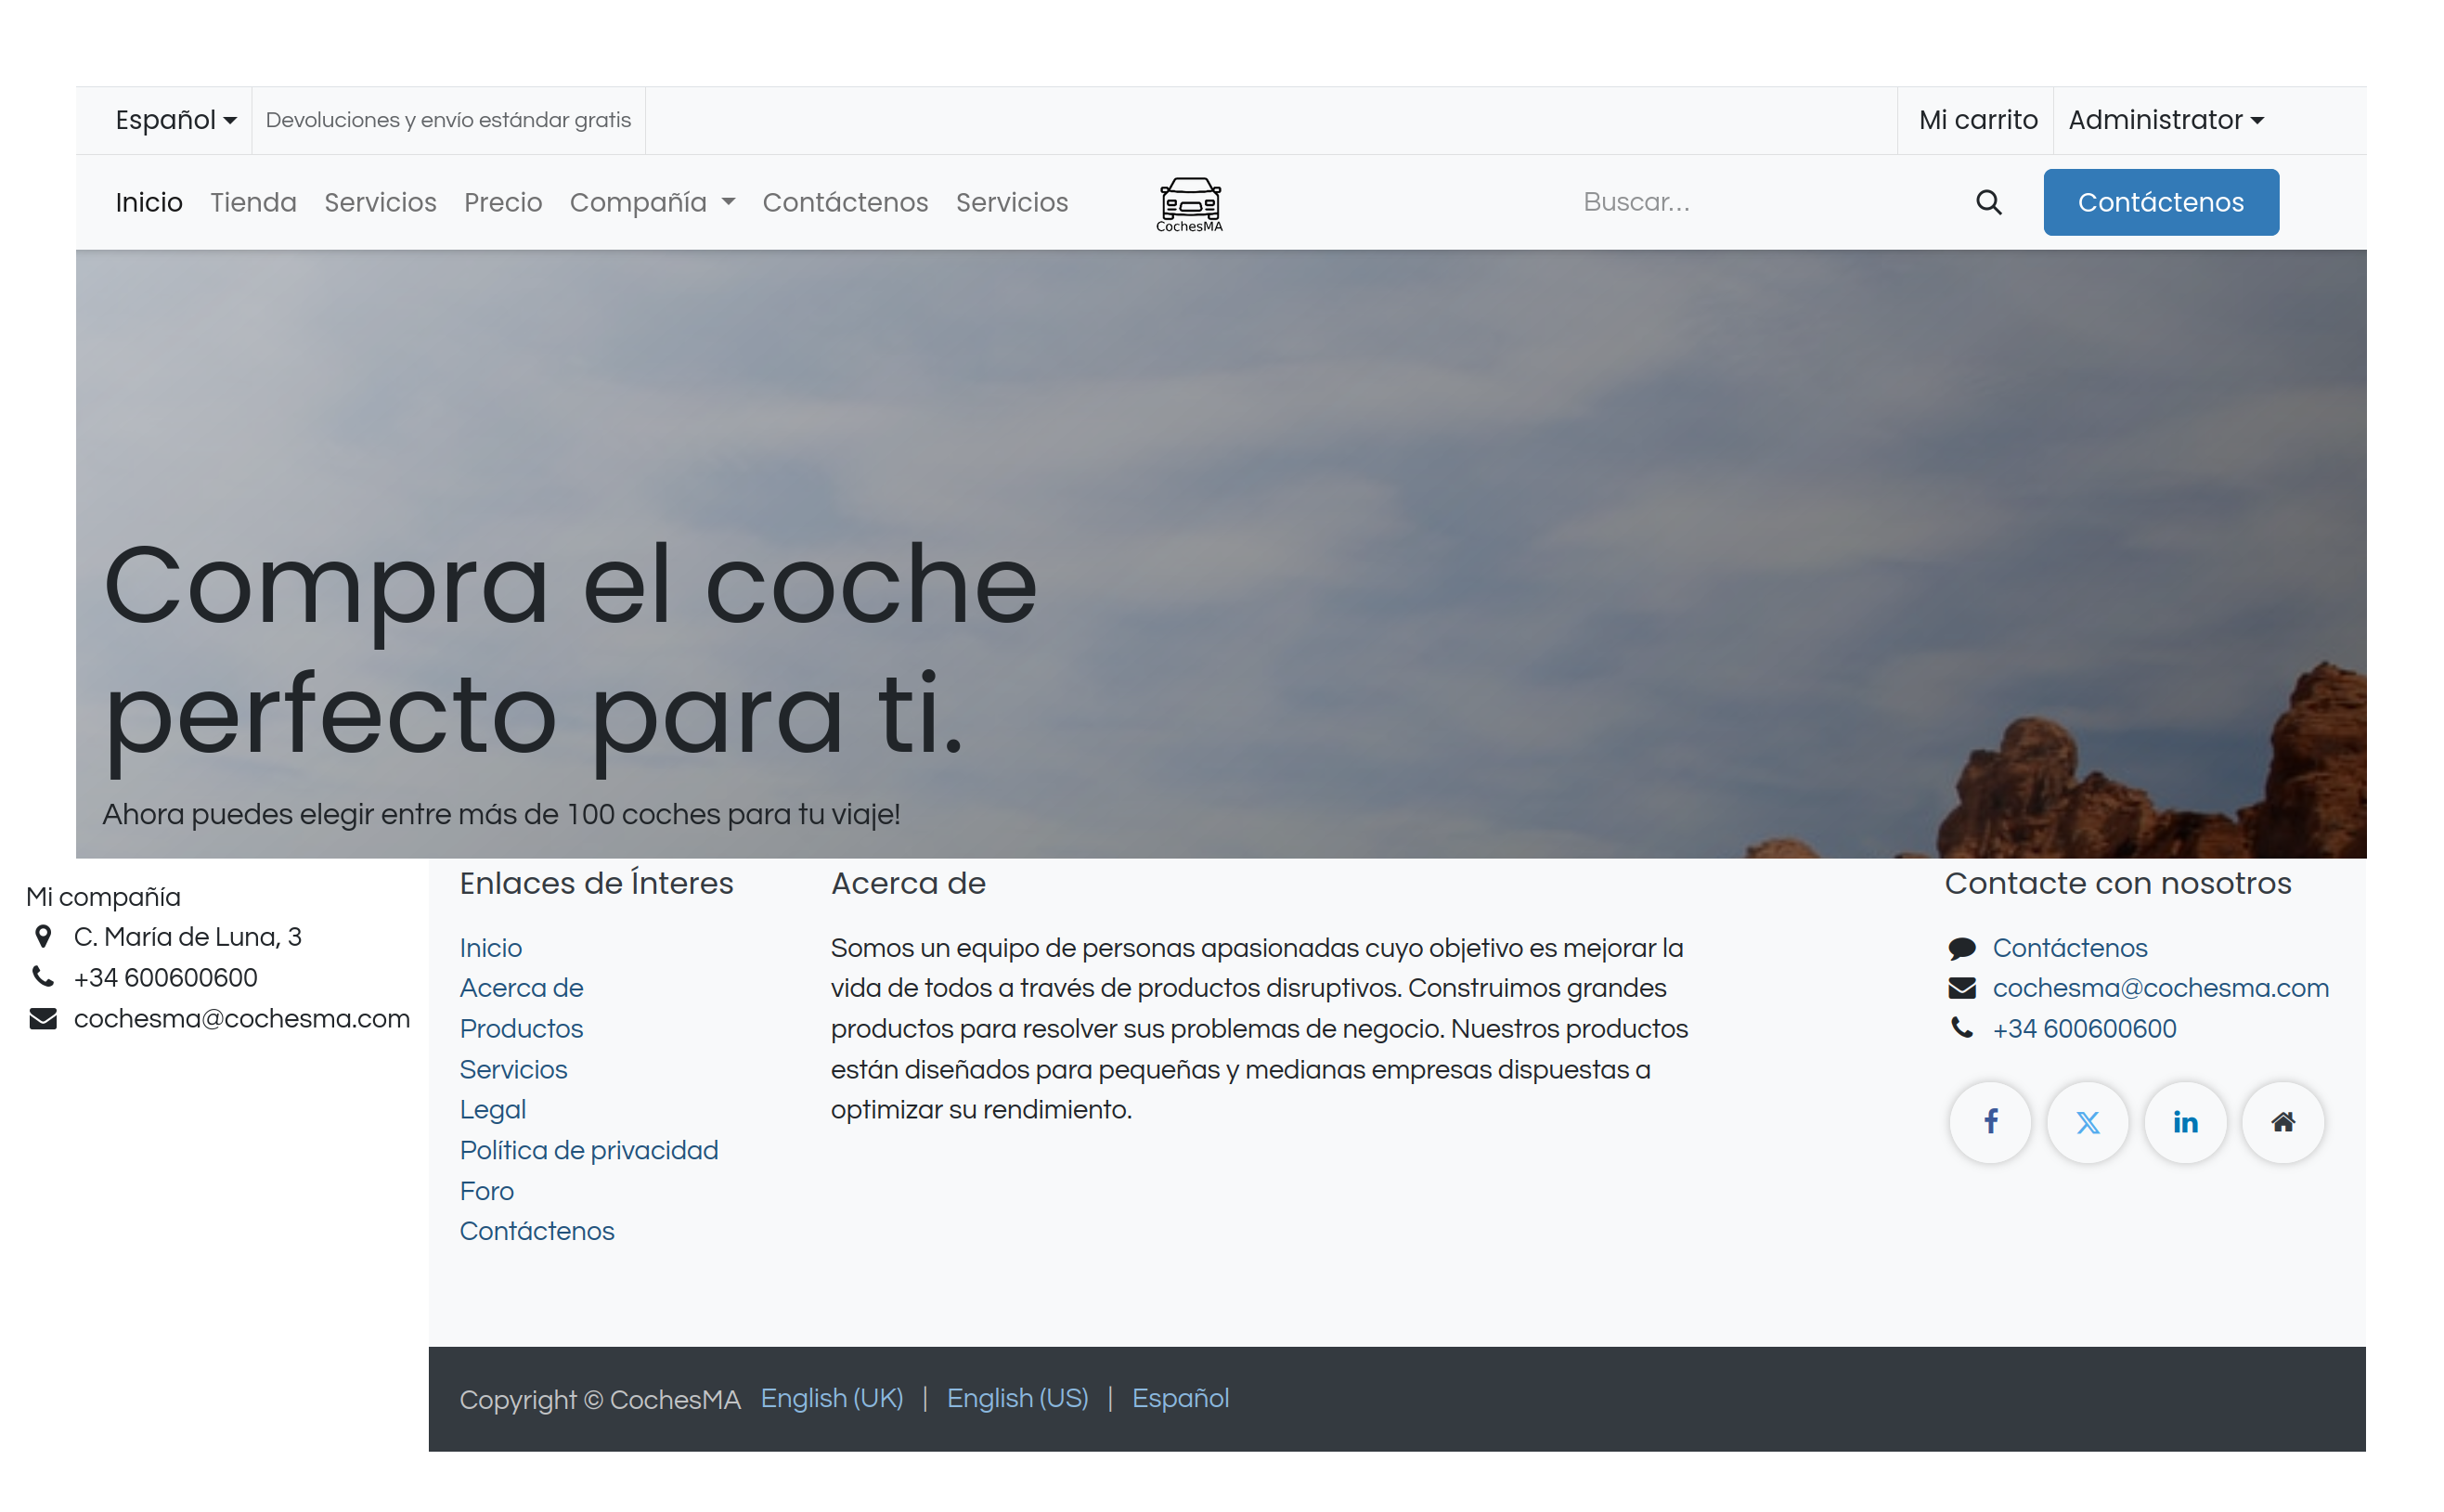
\includegraphics[width=1\linewidth]{fotosConfiguración/personalización.png}
    \caption{Personalizaciones de la web}
    \label{fig:enter-label}
\end{figure}

Además, se han realizado optimizaciones de SEO, para mejorar el ranking de la web en Google, para ello se ha añadido el logo, un título y una descripción adecuada y se han añadido palabras clave como alquiler, coche, viaje y en inglés, rent, car.
\newpage
\begin{figure}[h]
    \centering
    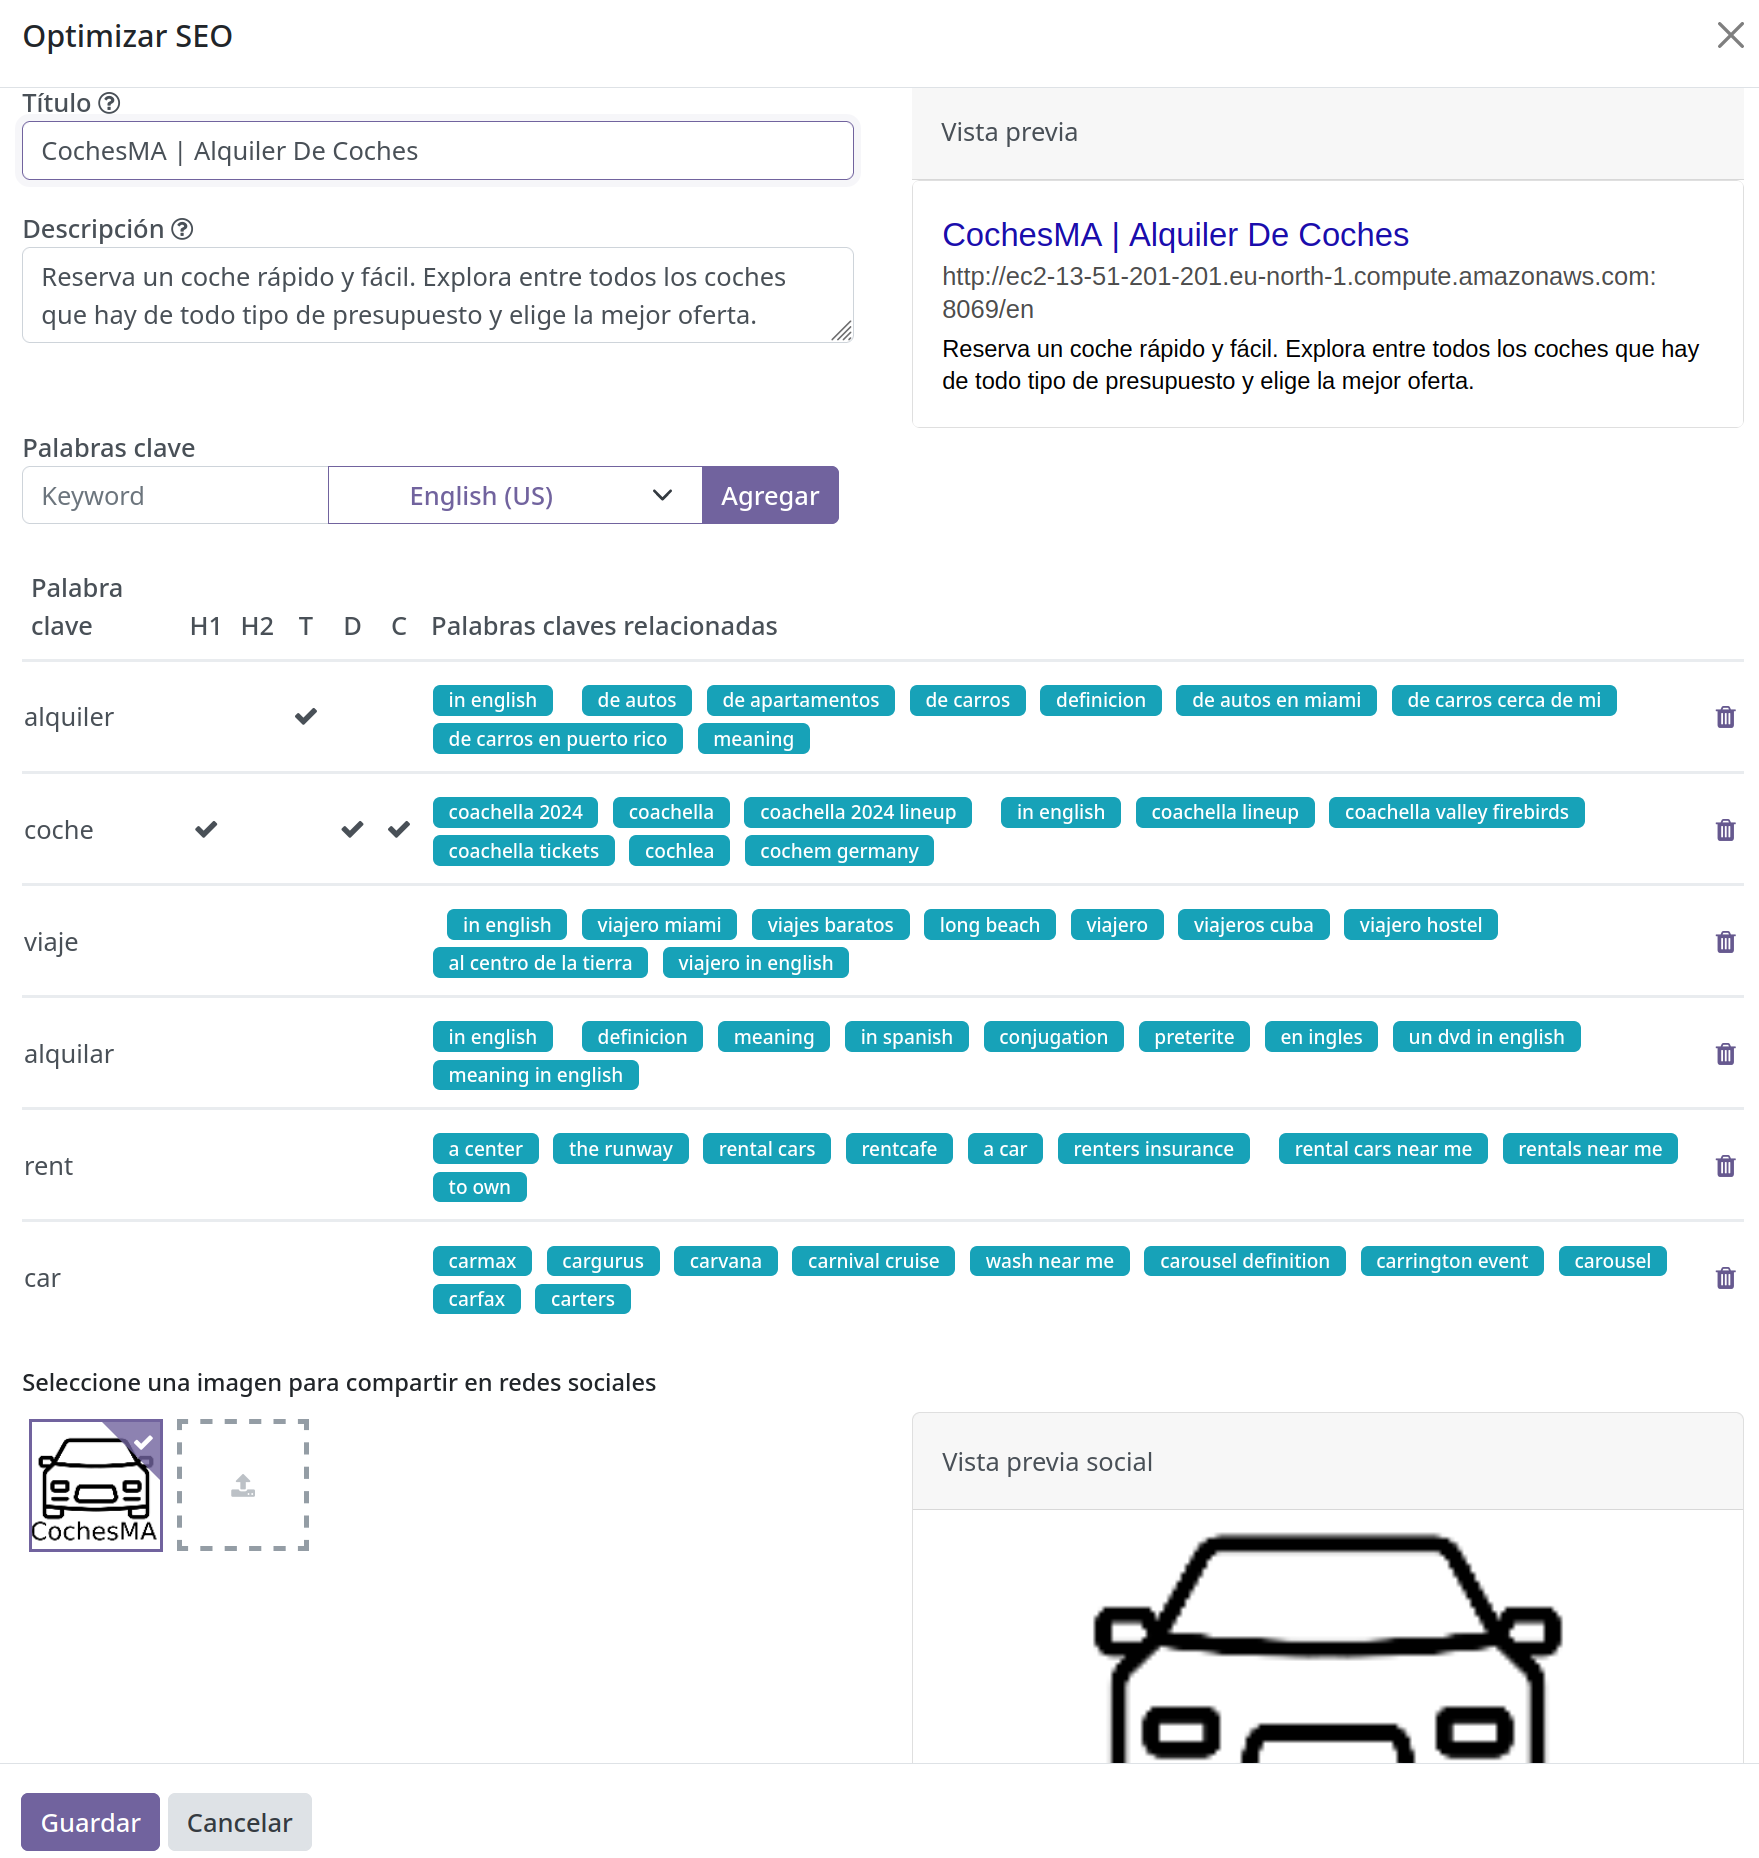
\includegraphics[width=1\linewidth]{fotosConfiguración/seo.png}
    \caption{Configuración del SEO}
    \label{fig:enter-label}
\end{figure}

\paragraph{}
Por último, hemos logrado implementar un servidor SSL localmente que nos permite acceder a nuestra web desde un dominio propio con conexión segura utilizando un servidor Nginx. 
\begin{figure}[h]
    \centering
    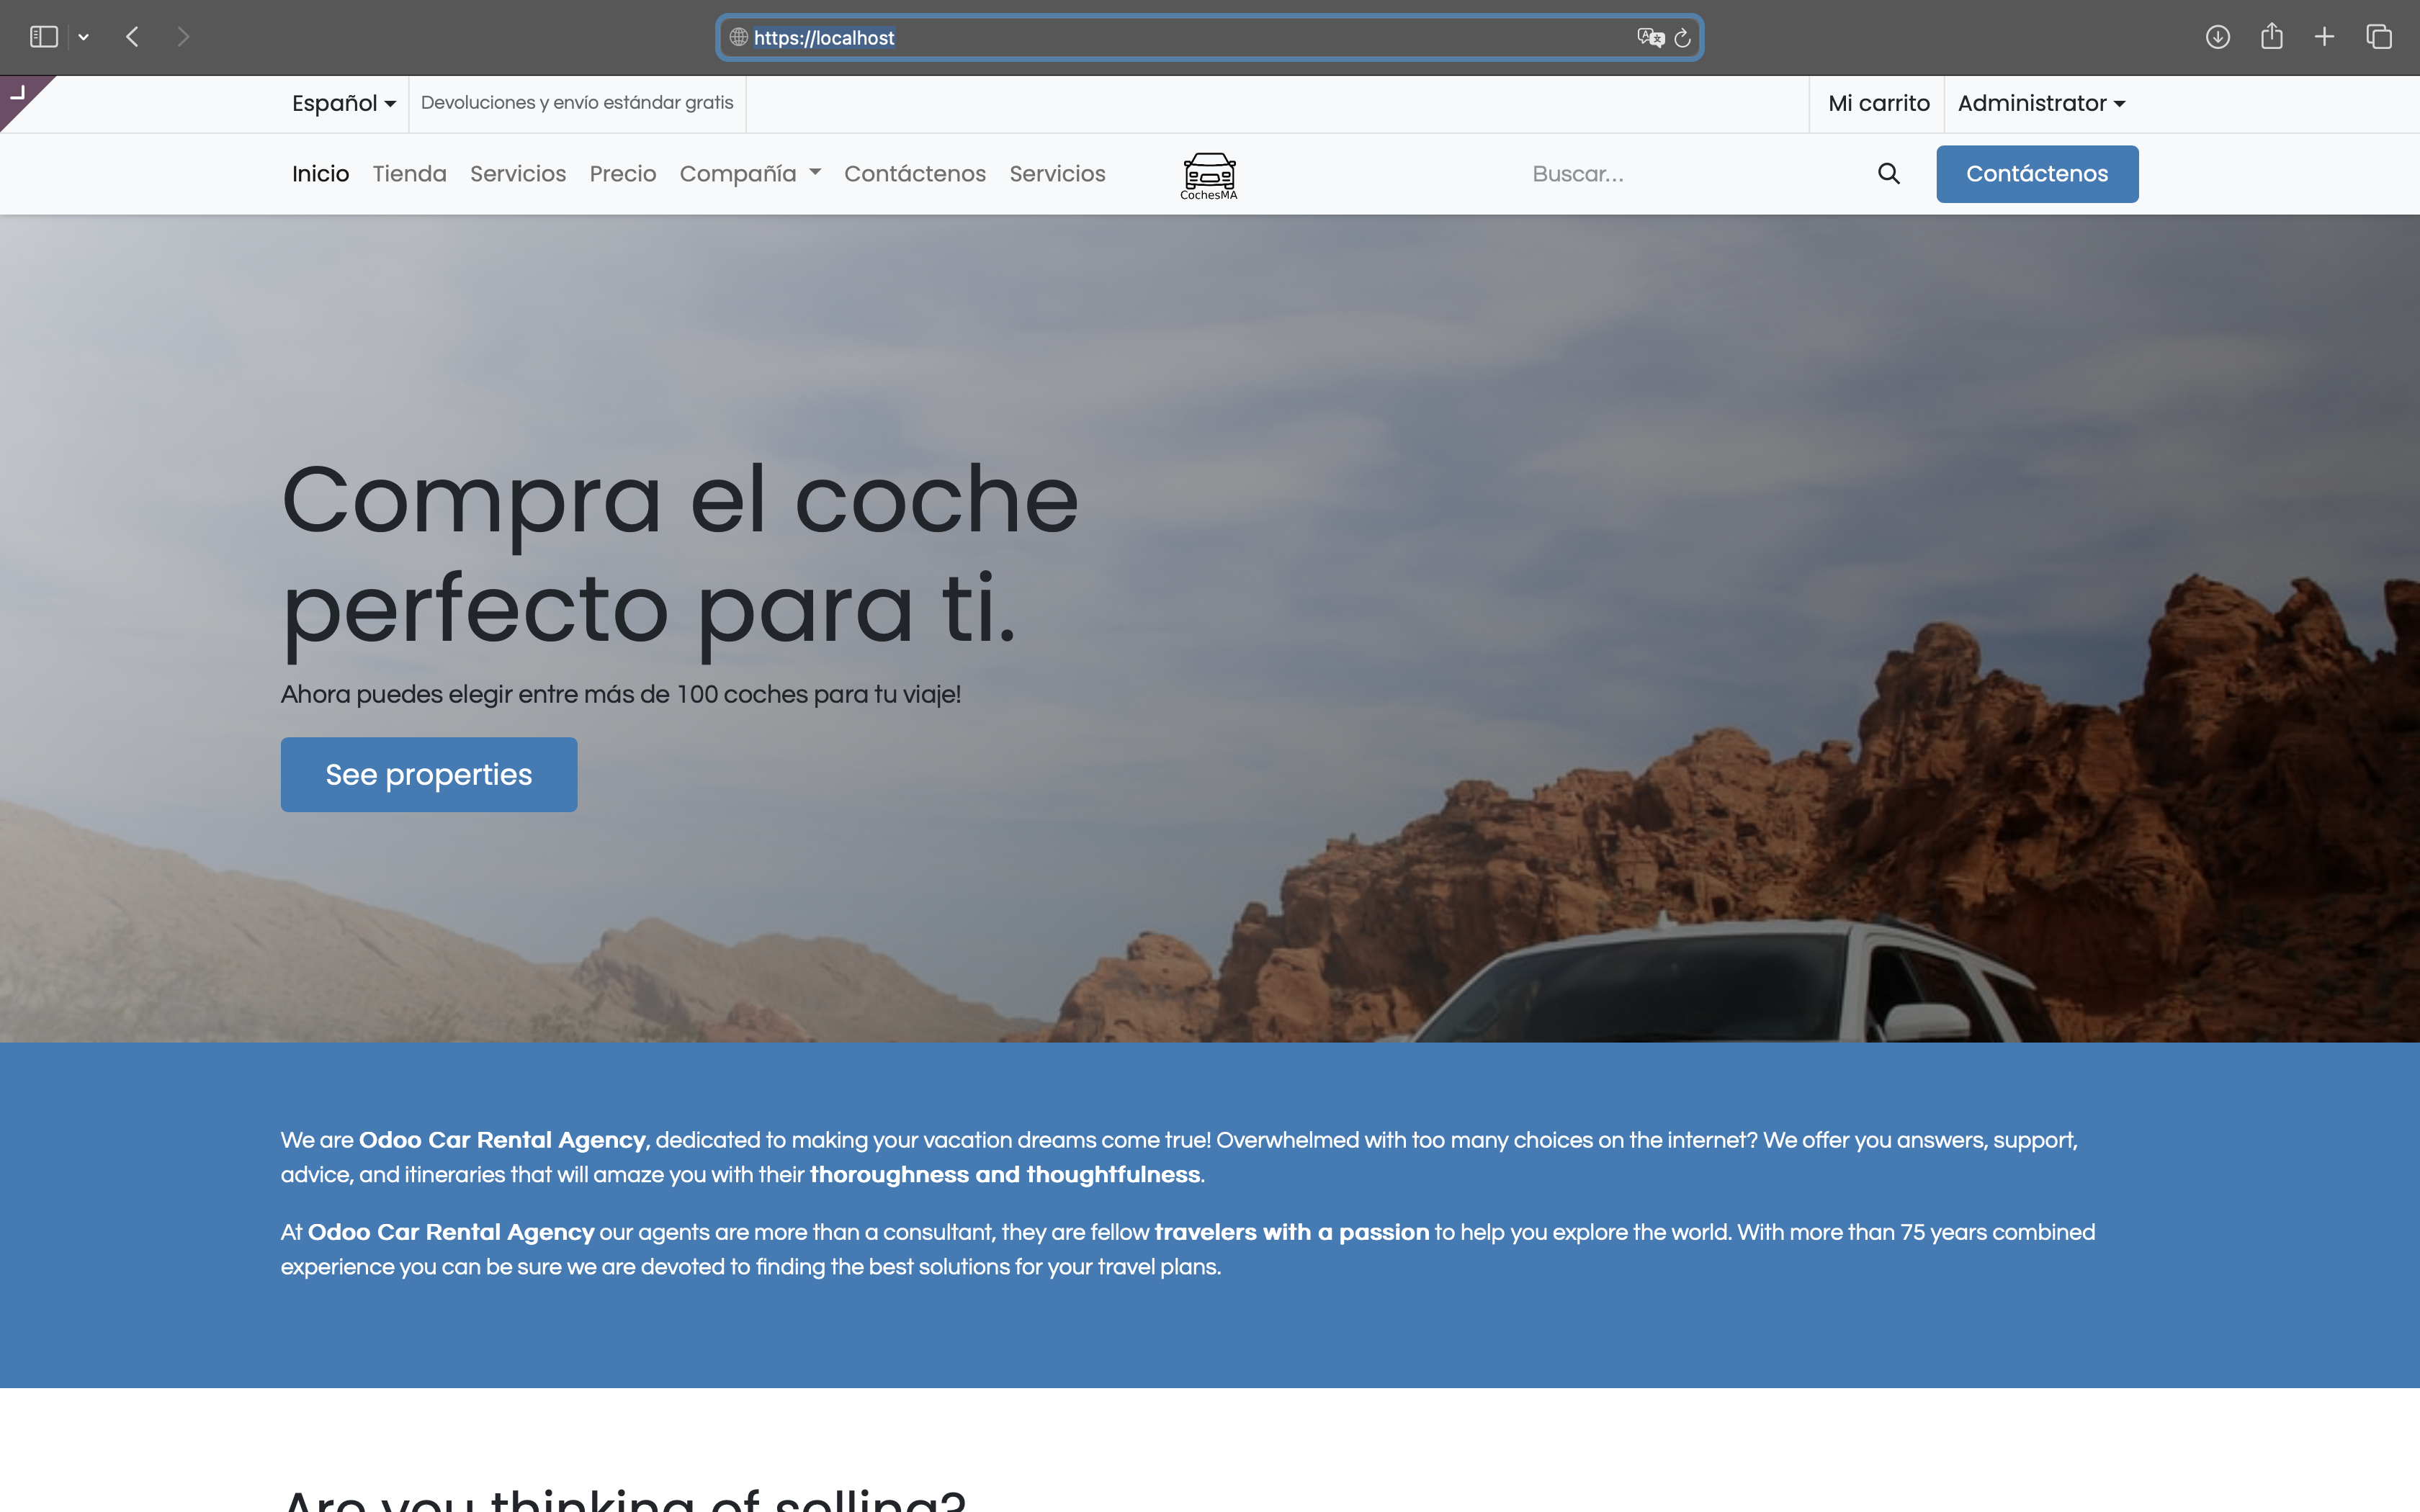
\includegraphics[width=1\linewidth]{SSL.png}
    \caption{Captura de pantalla del navegador con nuestra web en un dominio propio}
\end{figure}
\subsection{Conclusiones}
\paragraph{}
En cuanto al sistema multilingüe es sencillo la configuración pero tiene ciertas limitaciones, por ejemplo, no se ha conseguido que se traduzca todo el contenido de la página web como aquella información añadida manualmente. Aunque, permite traducir la mayoría de la pagina web lo suficiente para que se pueda navegar y realizar el servicio deseado. 
\paragraph{}
El proceso de personalización de la web es sencillo, intituitivo y ofrece una gran libertad posibilitando editar la página web y adecuarla a las necesidades de la compañía. En cuanto a la optimización del SEO es correcta permitiendo escalar la promoción de la web en el ranking del buscador. 
\paragraph{}
En referencia a la implementación de un servidor SSL para acceder desde un dominio propio con conexión HTTPS es muy sencillo y rápido. Únicamente se ha tenido que generar las claves, modificar el fichero utilizado para su configuración y añadir un segundo fichero. Este proceso sería similar para hacer en el entorno de despliegue. La gran diferencia es que el certificado utilizado no se puede auto firmar y se debe comprar para que sea validado por una entidad externa y los navegadores confíen en él.



%\section{Configuración técnica}
%\subsection{Copia de seguridad}
%\subsubsection{Autoevaluación}

%\subsubsection{Introducción}
%Este apartado aborda la gestión de las copias de seguridad en Odoo. Se va a hacer una evaluación de la configuración que ofrece para gestionar las bases de datos, la posibilidad de transferir los datos de Odoo de una instancia a otra y la capacidad de crear scripts para automatizar las copias de seguridad, las cuáles van a ser almacenadas en la nube.
%\subsubsection{Metodología}
%El primer paso que se ha realizado ha sido dirigirnos a la siguiente dirección en el navegador \textit{http://ec2-13-51-201-201.eu-north-1.compute.amazonaws.com:8069/web/database/manager}. Se ha hecho click en \textit{Set Master Password} y se ha introducido una contraseña que será necesaria en las operaciones que se van a realizar en este módulo. A continuación, Odoo ofrece una opción para crear una nueva base de datos, para ello se ha hecho click en \textit{Create Database} y se ha rellenado el formulario. Tras pulsar el botón de crear hay que esperar hasta que nos ha redirigido al inicio de sesión, una vez iniciado sesión con la información introducida anteriormente, ya puedes acceder a Odoo. También, ofrece una opción para duplicar una base de datos, para ello se ha pulsado en \textit{Duplicate} en la base de datos que se quiere duplicar y se ha introducido el nuevo nombre y la contraseña maestra, tras unos segundos se ha comprobado que se ha mostrado una nueva entrada en la lista de bases de datos, la cual tendrá la misma información que la original. Odoo nos da la posibilidad de eliminar bases de datos. En la lista se ha pulsado el botón \textit{Delete} del elemento que se quiere borrar y tras introducir la contraseña maestra se ha eliminado la base de datos. Por último, Odoo ofrece la posibilidad de realizar una copia de seguridad de las bases de datos. Para probar esta funcionalidad se ha hecho click en \textit{Backup} en la base de datos que se quiere realizar y se ha seleccionado el formato zip. Cómo resultado se descarga en la máquina un zip con la información de la base de datos. La capacidad de exportar la información junto con la posibilidad que ofrece Odoo de restaurar una base de datos, nos permite realizar transferencias de las bases de datos. Para comprobarlo se ha hecho una copia de seguridad de una de ellas como se ha explicado anteriormente y se ha enviado por WhatsApp. En otra máquina donde se tiene instalado Odoo, se ha accedido a WhatsApp y se ha descargado el zip. A continuación, nos hemos dirigido a \textit{http://localhost:8069/web/database/manager} y se ha hecho click en \textit{Restore Database}, se ha introducido la contraseña maestra y el nombre, se ha activado la opción de que la base de datos es una copia y se ha seleccionado el zip que contiene la información. Como resultado se ha creado una nueva entrada en la lista de bases de datos la cual contiene la información que se tenía en la otra máquina.
%\subsubsection{Resultados y análisis}
%Se ha conseguido realizar en Odoo la creación, eliminación, duplicación y copia de seguridad de una base de datos. Además, se ha conseguido transferir una base de datos de una instancia de Odoo a otra, mediante realización de una copia de seguridad de una base de datos y la restauración de la misma. 
%\subsubsection{Conclusiones}

%\newpage
%\subsection{Correo electrónico}
%\subsubsection{Autoevaluación}
%8
%\subsubsection{Introducción}
%Con el objetivo de permitir la comunicación de la empresa mediante Odoo se ha configurado un servidor de correo electrónico tanto saliente para poder enviar correos como entrante para poder recibirlos.
%\subsubsection{Metodología}
%Para crear un servidor SMTP y poder enviar correos a través de él, hay que ir a los ajustes de opciones generales, entrar en el menú de Servidores de correo saliente y crear un nuevo servidor. En este caso, se ha utilizado autentificación OAuth de Gmail, hay que asegurarse que se ha introducido \textit{odoo.com} en el campo Filtro DESDE, TLS como encriptación, \textit{smtp.gmail.com} como servidor SMTP y puerto 587. Se ha decidido utilizar un correo de UNIZAR para llevar a cabo la conexión con Gmail por lo que se ha puesto ese correo en el campo de nombre de usuario. A continuación, hay que insertar el ID y el Numero secreto en \textit{Usar un servidor de Gmail} en las opciones generales de los ajustes. Para ello, se ha ido a la siguiente web \textit{https://console.cloud.google.com/apis/} se ha iniciado sesión en gmail y se ha creado un nuevo proyecto llamado Odoo. Primero, en pantalla de consentimiento de OAuth se ha elegido el tipo de usuario externo, se han rellenao los formularios necesarios, cabe destacar que hay que añadir como dominio autorizado \textit{odoo.com}. A continuación, se ha ido al menú \textit{Crear credenciales} y se ha seleccionado la opción OAuth client ID. En este menú se ha elegido la opción \textit{Aplicación web} y se ha añadido como URIS de redirección autorizadas \textit{http://ec2-13-51-201-201.eu-north-1.compute.amazonaws.com:8069/google\_gmail/confirm} . En la misma pantalla se mostrará el \textit{ID} y \textit{Secreto} con los que hay que rellenar los campos en Odoo. En la pantalla del servidor de correo que se estaba creando la prueba de conexión será exitosa. Por otro lado, el proceso de añadir un servidor de correo entrante es similar. Cabe destacar que en el campo de nombre del servidor se ha introducido \textit{imap.gmail.com} y se ha activado la opción SSL/TLS. Para llevar a cabo el proceso de envío de un correo electrónico desde Odoo y probar el servidor de salida se ha instalado el módulo Contactos. En este módulo se muestra todos los contactos de empleados, empresas, individuos que se ha tenido. Si se hace click en un contacto, se podrá ver a la derecha un chat en el que se ha escrito un correo y se ha enviado.
%\subsubsection{Resultados y análisis}
%\subsubsection{Conclusiones}

\newpage

\newpage
\section{Configuración técnica - Copia de seguridad}
\subsection{Autoevaluación}
En esta sección se han cumplido los objetivos correspondientes al 10.
\subsection{Introducción}
\paragraph{}
Este apartado aborda la gestión de las copias de seguridad en Odoo. Se va a hacer una evaluación de la configuración que ofrece para gestionar las bases de datos, la posibilidad de transferir los datos de Odoo de una instancia a otra y la capacidad de crear scripts para automatizar las copias de seguridad, las cuáles van a ser almacenadas en la nube.
\subsection{Metodología}
\paragraph{}
El primer paso que se ha realizado ha sido dirigirnos a la siguiente dirección en el navegador:\\ \href{http://ec2-13-51-201-201.eu-north-1.compute.amazonaws.com:8069/web/database/manager}{http://ec2-13-51-201-201.eu-north-1.compute.amazonaws.com:8069/web/database/manager}. Se ha hecho click en \textit{Set Master Password} y se ha introducido una contraseña que será necesaria en las operaciones que se van a realizar en este módulo.
\paragraph{}
A continuación, Odoo ofrece una opción para crear una nueva base de datos, para ello se ha hecho click en \textit{Create Database} y se ha rellenado el formulario. Tras pulsar el botón de crear hay que esperar hasta que nos ha redirigido al inicio de sesión, una vez iniciado sesión con la información introducida anteriormente, ya puedes acceder a Odoo. 
\paragraph{}
También, ofrece una opción para duplicar una base de datos, para ello se ha pulsado en \textit{Duplicate} en la base de datos que se quiere duplicar y se ha introducido el nuevo nombre y la contraseña maestra, tras unos segundos se ha comprobado que se ha mostrado una nueva entrada en la lista de bases de datos, la cual tendrá la misma información que la original.
\paragraph{}
Odoo nos da la posibilidad de eliminar bases de datos. En la lista se ha pulsado el botón \textit{Delete} del elemento que se quiere borrar y tras introducir la contraseña maestra se ha eliminado la base de datos. Por último, Odoo ofrece la posibilidad de realizar una copia de seguridad de las bases de datos. Para probar esta funcionalidad se ha hecho clic en \textit{Backup} en la base de datos que se quiere realizar y se ha seleccionado el formato zip. Cómo resultado se descarga en la máquina un zip con la información de la base de datos. 
\paragraph{}
La capacidad de exportar la información junto con la posibilidad que ofrece Odoo de restaurar una base de datos, nos permite realizar transferencias de las bases de datos. Para comprobarlo se ha hecho una copia de seguridad de una de ellas como se ha explicado anteriormente y se ha enviado por WhatsApp. En otra máquina donde se tiene instalado Odoo, se ha accedido a WhatsApp y se ha descargado el zip. A continuación, hemos abierto en nuestro navegador la instancia de odoo localmente y nos hemos dirigido a \textit{http://localhost:8069/web/database/manager} y se ha hecho click en \textit{Restore Database}, se ha introducido la contraseña maestra y el nombre, se ha activado la opción de que la base de datos es una copia y se ha seleccionado el zip que contiene la información. Como resultado se ha creado una nueva entrada en la lista de bases de datos la cual contiene la información que se tenía en la otra máquina.

\paragraph{}
Los pasos descritos nos permiten realizar la copia de seguridad de forma manual, sin embargo, creemos que esto no es viable para una empresa. Esta tarea se debe automatizar asegurándonos su correcto funcionamiento. Para ello hemos realizado el siguiente script en nuestra máquina remota:

\begin{lstlisting}[frame=single, basicstyle=\tiny]
#!/bin/bash
# vars
BACKUP_DIR=/home/ubuntu/sisInfo2_proyect/backups
ODOO_DATABASE=GOOD
ADMIN_PASSWORD=adminadmin

# create a backup directory
mkdir -p ${BACKUP_DIR}

# create a backup
curl -X POST \
    -F "master_pwd=${ADMIN_PASSWORD}" \
    -F "name=${ODOO_DATABASE}" \
    -F "backup_format=zip" \
    -o ${BACKUP_DIR}/${ODOO_DATABASE}.$(date +%F_%H-%M-%S).zip \
    http://localhost:8069/web/database/backup

# push to github
cd /home/ubuntu/sisInfo2_proyect
git pull
git add .
git commit -m "backup $(date +%F_%H-%M-%S)"
git push
\end{lstlisting}

\paragraph{}
En este script hecho con \textit{Bash} lo primero que hacemos es definir las variables, facilitando cualquier posible cambio de nombre o ruta en un futuro. A continuación se realiza la copia de seguridad y se almacena en el directorio definido anteriormente. Por último, se hace un commit a un repositorio de Github donde se encuentran todas las copias de seguridad realizadas. De esta forma tenemos almacenadas todas nuestras copias de seguridad en un lugar distinto a nuestra máquina remota. Por tanto, conseguimos que en caso de cualquier imprevisto tenemos una copia de seguridad alejada físicamente de nuestro sistema funcional. Cabe destacar que para poder realizar el commit desde la máquina remota se ha tenido que clonar el repositorio y permitir realizar commits. Para ello hemos utilizado la herramienta que nos proporciona Github; \href{https://docs.github.com/es/github-cli/github-cli/quickstart}{GitHub CLI}. 
\paragraph{}
El segundo paso en el proceso de automatizar esta tarea es ejecutar este script de forma regular y automática. Para ello, hemos creado un demonio que se encarga de ejecutarlo cada día a la una de la madrugada. Para ello hemos ejecutado el siguiente comando:
\begin{lstlisting}[frame=single, basicstyle=\tiny]
crontab -e
\end{lstlisting}
\paragraph{}
Y con el editor de texto añadimos la siguiente línea:
\begin{lstlisting}[frame=single, basicstyle=\tiny]
0 1 * * * /home/ubuntu/script.sh
\end{lstlisting}
\paragraph{}
Con esta línea indicamos que a la 1:00 de cada día se ejecuta el script que se encuentra en esa dirección, por lo tanto, en caso de cambiar de lugar el script se debería modificar esa línea también.

\subsection{Resultados y análisis}
\paragraph{}
Se ha conseguido realizar en Odoo la creación, eliminación, duplicación y copia de seguridad de una base de datos. 
\begin{figure}[h]
    \centering
    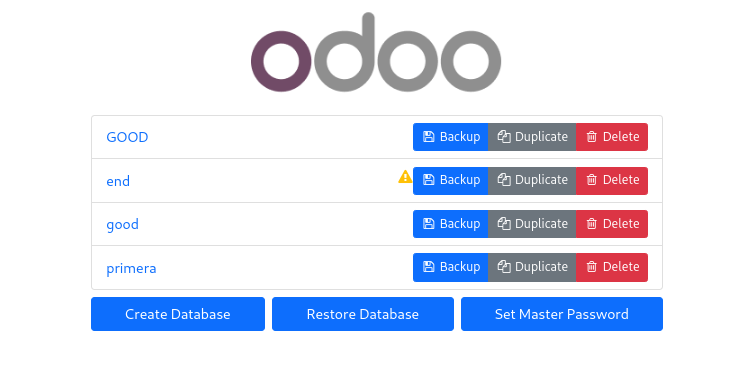
\includegraphics[width=1\linewidth]{fotosConfiguración/bases.png}
    \caption{Historial de commits del repositorio}
\end{figure}
\paragraph{} Además, se ha conseguido transferir una base de datos de una instancia de Odoo a otra, mediante realización de una copia de seguridad de una base de datos y la restauración de la misma. 
\paragraph{}
Por último hemos conseguido automatizar esta tarea, creando un script, generando un demonio en nuestra máquina remota y almacenándolas en una lugar físico distinto a la máquina remota. Como lugar de almacenamiento remoto hemos elegido Github, como hemos comentado previamente. Esta decisión se ha basado en la facilidad de subir las copias de seguridad, el control de versiones y que podemos acceder desde cualquier lugar con conexión, ya que el repositorio donde la estamos almacenando es público. El control de versiones nos permite en todo momento acceder a la versión de cualquier día. Si observamos el historial de commits de \href{https://github.com/Practicass/sisInfo2_proyect/commits/main/}{nuestro repositorio} podemos recuperar cualquier copia de seguridad. 
\begin{figure}[h]
    \centering
    
\includegraphics[width=1\linewidth]{backup/commits.png}
    \caption{Historial de commits del repositorio}
\end{figure}
\subsection{Conclusiones}
\paragraph{}
En esta sección hemos analizado las herramientas que ofrece Odoo para gestionar las bases de datos. Se ha comprobado cómo se puede realizar la copia de seguridad de nuestro ERP. Odoo tiene sistema de backup muy sencillo e intitutivo. Que nos permite tener en todo momento nuestra base de datos replicada. Consideramos que es fundamental que estas \textit{backups} no se encuentren en el mismo lugar físico que la base de datos, ya que en caso de una catástrofe como puede ser un incendio de los servidores en los que tenemos nuestra base de datos, en nuestro caso, los servidores de AWS de Estocolmo; perderíamos todo. En cambio, al tener las copias de seguridad en un lugar físico tendríamos la capacidad de recomponer el sistema en minutos.

\paragraph{}
Además tener copias de seguridad no solo nos previene de catástrofes inesperadas, también de nuestros errores. Durante las últimas semanas de elaboración de este análisis cometimos un error que nos causo problemas y no conseguíamos deshacer los pasos que habíamos realizado. Es por ello, que tomamos la decisión de volver a una versión antigua y utilizar una de las copias de seguridad que se habían realizado.
\newpage
\section{Configuración técnica - Correo electrónico}
\label{sec:correo}
\subsection{Autoevaluación}
En esta sección se han cumplido los objetivos correspondientes al 10.
\subsection{Introducción}
\paragraph{}
Con el objetivo de permitir la comunicación de la empresa mediante Odoo se ha configurado un servidor de correo electrónico tanto saliente para poder enviar correos como entrante para poder recibirlos.
\subsection{Metodología}
\paragraph{}
Para crear un servidor SMTP y poder enviar correos a través de él, hay que ir a los ajustes de opciones generales, entrar en el menú de Servidores de correo saliente y crear un nuevo servidor. En este caso, se ha utilizado autentificación OAuth de Gmail, hay que asegurarse que se ha introducido \textit{odoo.com} en el campo Filtro DESDE, TLS como encriptación, \textit{smtp.gmail.com} como servidor SMTP y puerto 587. Se ha creado un correo para llevar a cabo la conexión con Gmail por lo que se ha puesto ese correo en el campo de nombre de usuario. 
\paragraph{}
A continuación, hay que insertar el ID y el Numero secreto en \textit{Usar un servidor de Gmail} en las opciones generales de los ajustes. Para ello, se ha ido a la siguiente web \href{https://console.cloud.google.com/apis/}{https://console.cloud.google.com/apis/} se ha iniciado sesión en Gmail y se ha creado un nuevo proyecto llamado Odoo. Primero, en pantalla de consentimiento de OAuth se ha elegido el tipo de usuario externo, se han rellenado los formularios necesarios, cabe destacar que hay que añadir como dominio autorizado \textit{odoo.com}. A continuación, se ha ido al menú \textit{Crear credenciales} y se ha seleccionado la opción OAuth client ID. En este menú se ha elegido la opción \textit{Aplicación web} y se ha añadido como URIS de redirección autorizadas \textit{http://ec2-13-51-201-201.eu-north-1.compute.amazonaws.com:8069/google\_gmail/confirm} . En la misma pantalla se mostrará el \textit{ID} y \textit{Secreto} con los que hay que rellenar los campos en Odoo. 
\paragraph{}
En la pantalla del servidor de correo que se estaba creando la prueba de conexión será exitosa. Por otro lado, el proceso de añadir un servidor de correo entrante es similar. Cabe destacar que en el campo de nombre del servidor se ha introducido \textit{imap.gmail.com} y se ha activado la opción SSL/TLS. Además, hay que ir a los ajustes de Gmail y habilitar IMAP, desde el apartado \textit{Reenvío e IMAP/POP}. 
\paragraph{}
Para llevar a cabo el proceso de envío de un correo electrónico desde Odoo y probar el servidor de salida se ha instalado el módulo Contactos. En este módulo se muestra todos los contactos de empleados, empresas, individuos que se ha tenido. Si se hace click en un contacto, se podrá ver a la derecha un chat en el que se ha escrito un correo y se ha enviado. Además, si se produce una respuesta a ese correo aparecerá en el mismo chat. 
\subsection{Resultados y análisis}
\paragraph{}
Se ha conseguido configurar un servidor SMTP mediante Gmail y autentificación OAuth de Gmail. Se ha realizado el envío de un correo electrónico desde Odoo mediante el servidor de correo saliente.
\begin{figure}[h]
    \centering
    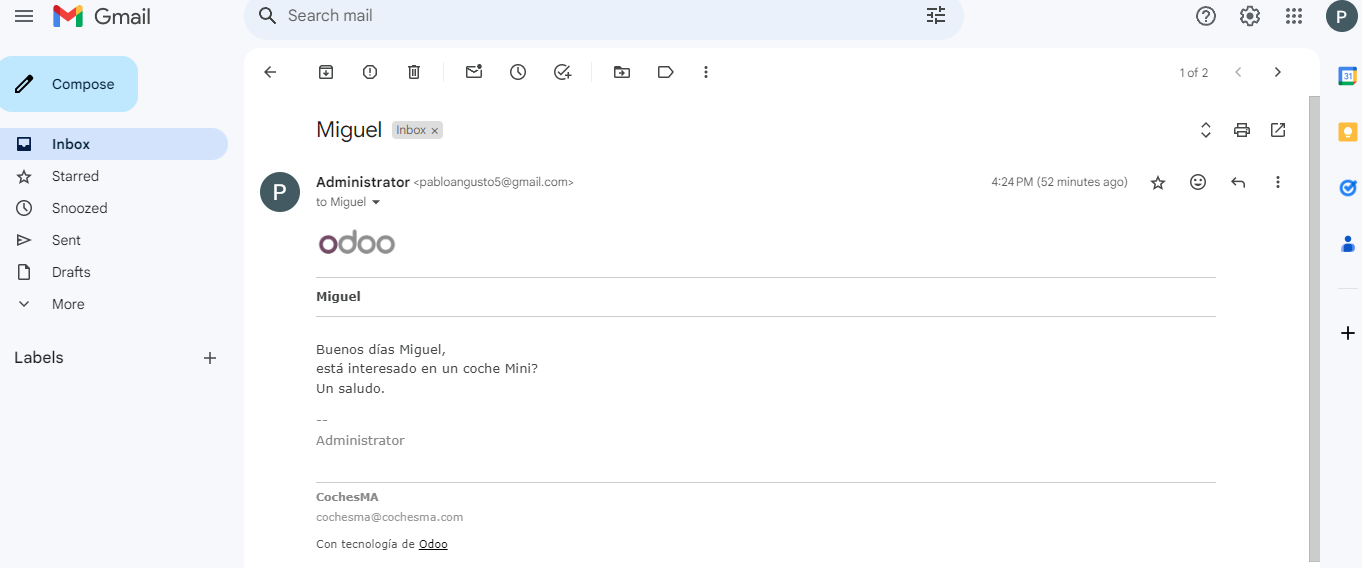
\includegraphics[width=1\linewidth]{fotosConfiguración/correoEnvio1.png}
    \caption{Correo saliente desde bandeja de salida}
    \label{fig:enter-label}
\end{figure}
\newpage
\begin{figure}[h]
    \centering
    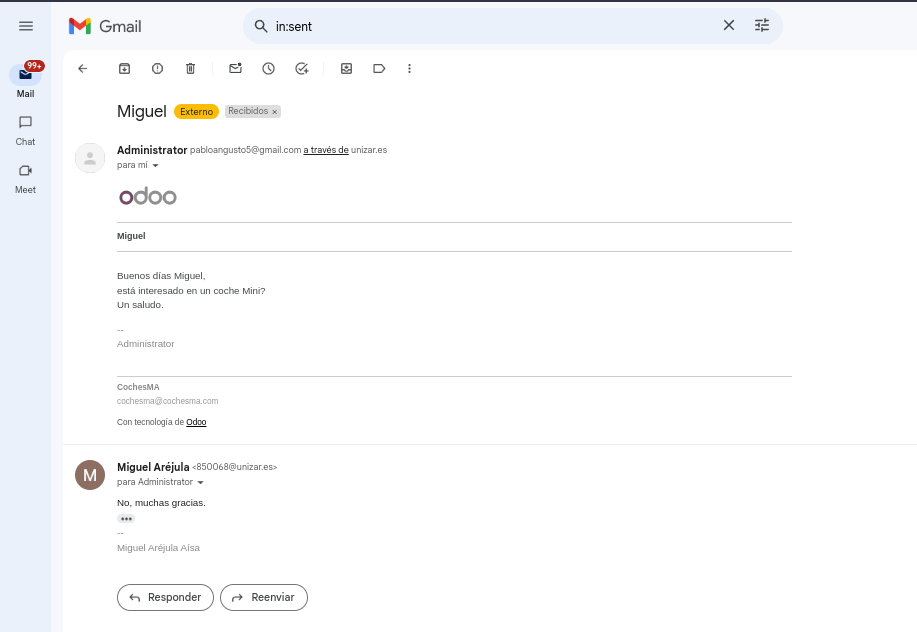
\includegraphics[width=1\linewidth]{fotosConfiguración/capturaCorreoMiguel.png}
    \caption{Correo saliente desde bandeja de salida}
    \label{fig:enter-label}
\end{figure}
\paragraph{}
Además, se ha comprobado el correcto funcionamiento del servidor de correo entrante como se muestra en la siguiente figura.
\begin{figure}[h]
    \centering
    
\includegraphics[width=0.8\linewidth]{fotosConfiguración/correoOdoo.png}
    \caption{Conversación de correos desde Odoo}
    \label{fig:enter-label}
\end{figure}
\paragraph{}
Por último, se examinaron las capacidades de automatización de Odoo en relación con la gestión de correos electrónicos. Esta funcionalidad específica de Odoo se encuentra disponible a través del módulo \textit{Studio}, el cual no está habilitado en la versión de Docker de Odoo, sino únicamente en la versión en la nube. Mediante este módulo, es posible establecer reglas que se activan en función de eventos internos del sistema o de los correos electrónicos recibidos por el sistema.
Cabe destacar qué en el modulo de \textit{Ventas} existe una funcionalidad similar a la del módulo Studio, que permite generar iniciativas a partir de correos pero no cubre los requisitos planteados.
\subsection{Conclusiones}
\paragraph{}
La configuración y gestión de correos electrónicos en Odoo se muestran como procesos accesibles y bien estructurados, lo que permite una integración eficiente con proveedores externos como Google y una comunicación fluida dentro de la plataforma.
\paragraph{}
Las configuraciones que se han realizado en este módulo, son algo complejas, en especial si nunca se ha utilizado una cuenta de Gmail para realizar este tipo de funcionalidades. Además, requiere configuraciones fuera de Odoo tanto en Google Cloud como en Gmail esto añade dificultad a la hora de realizar este módulo. Sin embargo, es una tarea que resulta importante porque tiene un gran impacto en la comunicación de la compañía. Mediante la configuración del servidor saliente SMTP y el servidor entrante IMAP de manera precisa se garantiza una comunicación adecuada con el servicio de correo. Una vez configurados los servidores de correo, Odoo permite enviar y recibir mensajes directamente desde la plataforma, simplificando así la gestión de la comunicación interna y externa de la empresa.
\paragraph{}
Es importante destacar que la configuración del servidor de correo entrante IMAP puede presentar algunos problemas, ya que se ha realizado este proceso con los correos de UNIZAR y no ha tenido un correcto funcionamiento por lo que habría que tener presente esta posibilidad con los correos de empresa y que igual implica alguna configuración más.
\paragraph{}
En cuanto a las capacidades de automatización, aunque se puedan implementar con alguna solución en local están limitadas a usar el módulo \textit{Studio} de la versión en la nube. Permite acciones específicas en función de eventos internos del sistema o correos electrónicos recibidos, aunque no está disponible en la versión de Docker.










\section{Gestión de proyectos}

\subsection{Autoevaluación}
\paragraph{}
En esta sección se han cumplido los objetivos correspondientes al 10.

\subsection{Introducción}
\paragraph{}
La organización de las tareas dentro de un equipo es esencial para lograr los objetivos con éxito. Odoo ofrece una herramienta fácil, visual e intuitiva para gestionar las diferentes tareas de cada equipo de trabajo dentro de nuestra empresa.

\subsection{Metodología}
\paragraph{}
Para utilizar este módulo, primero debemos instalarlo. Al igual que el resto de módulos, nos dirigimos a la pantalla de las aplicaciones y buscamos e instalamos el módulo \textit{Proyecto}. Una vez instalado, podemos abrirlo en la esquina superior izquierda. Se mostrará la ventana principal en la cual aparecerán nuestros proyectos, al ser la primera vez que se abre se encuentra vacía. Se debe pulsar en el botón \textit{Nuevo}, rellenar el formulario con el nombre del proyecto deseado y pulsar el botón de crear. Se abrirá automáticamente la página del proyecto recién creado. Lo primero que debemos hacer para comenzar a gestionar nuestro proyecto es crear las columnas para clasificar las tareas. En nuestro caso, hemos decidido dividirlas en tres estados: \textit{Pendiente}, \textit{En proceso} y \textit{Hecho}. Para crear las columnas, se pulsa en el botón \textit{+ Etapa} y se escribe el nombre. Por último, se debe realizar una configuración previa para poder utilizarlo para gestionar nuestras tareas. Nos dirigimos a la ventana de ajustes y seleccionamos \textit{Proyecto}. Aparecerán varias opciones que podemos añadir, en nuestro caso, hemos decidido utilizar la \textit{Dependencia de tareas}. Esta opción permite determinar el orden de las tareas y bloquearlas hasta que se hayan completado con éxito otras tareas.
\paragraph{}
Tras realizar la configuración pertinente al módulo, podemos hacer uso de él. En el proyecto deseado se crean las tareas y se colocan en la columna que corresponda. En un primer momento, las tareas se encontrarán en el estado \textit{Pendiente} y según vaya avanzando el tiempo, las tareas se irán cambiando de columna. Las tareas pueden ser asignadas a miembros del equipo, pueden tener una fecha límite, etiquetas, subtareas, bloqueos y pueden ser prioritarias. Todas estas configuraciones se hacen seleccionando la tarea y modificando los campos deseados. Estas configuraciones nos facilitan la organización de las tareas y tener muy claro de forma visual qué es lo que hay que hacer, en qué tiempo, quién está realizando cada tarea y el flujo de trabajo del equipo.

\subsection{Resultados y análisis}
\paragraph{}
Como hemos mencionado previamente, es fundamental organizar las tareas para cumplir con el plazo y realizar todas las tareas. Durante la realización del análisis de Odoo y la creación de la memoria, hemos decidido utilizar este módulo, consiguiendo evaluarlo de la mejor forma posible y obteniendo las ventajas del módulo para nuestro proyecto.
\paragraph{}
Hemos decidido organizar el tablero con tres columnas: \textit{Pendiente}, \textit{En proceso} y \textit{Hecho}. La primera son aquellas tareas que no se han empezado a realizar, en la segunda se encuentran las tareas que se están realizando y en la última las tareas que han sido completadas. Cada tarea, a su vez, está dividida en cuatro subtareas, cada subtarea corresponde con los objetivos marcados, obtener un cinco, un siete, un ocho o un diez. Todas las tareas tienen como fecha límite el día previo a la entrega, salvo la última tarea (\textit{Memoria final}) que tiene como fecha límite el día de la entrega. Además, se han etiquetado según el grado de dificultad que hemos considerado, pudiendo ser: \textit{Hard}, \textit{Medium} e \textit{Easy}. En nuestro caso, no hemos asignado las tareas a ningún miembro ya que desde el comienzo del proyecto hemos decidido realizar todas las tareas de forma conjunta. Es cierto que al tener que trabajar de forma simultánea nos puede costar más tiempo, sin embargo, consideramos que de esta forma ambos integrantes del equipo aprendemos todas las funcionalidades que nos ofrece este ERP y nos ayudamos mutuamente. También hemos decidido que la tarea más prioritaria es la \textit{Memoria final}, ya que es la tarea a entregar y que hay que cumplir con el plazo. Además, esta tarea tiene una dependencia con las otras tareas. No se puede realizar hasta que todas las tareas de los módulos se hayan completado.

\begin{figure}[h]
    \centering
    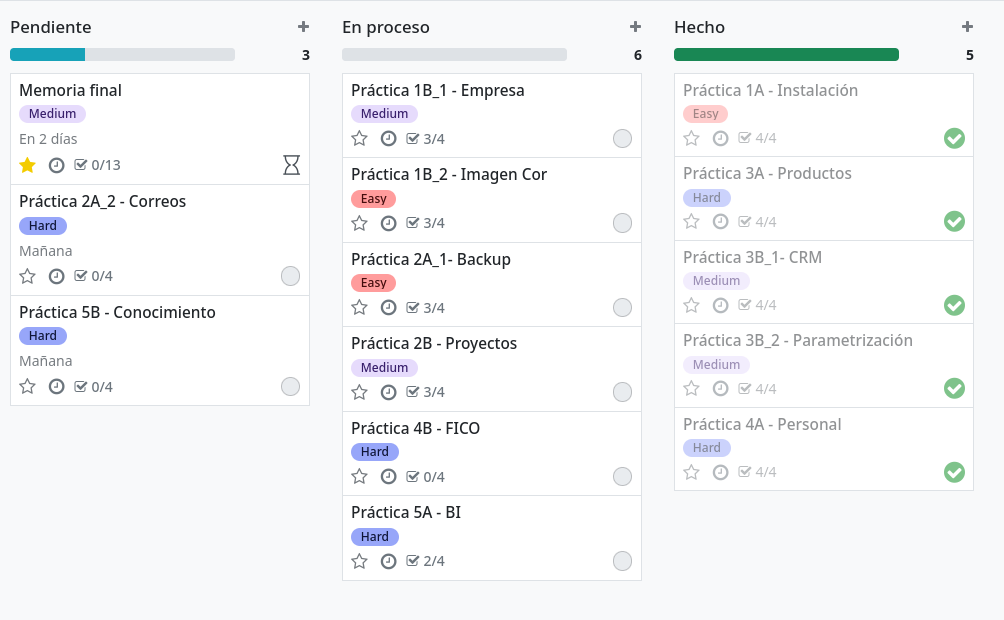
\includegraphics[width=1\linewidth]{proyecto.png}
    \caption{Vista Kanban de nuestro proyecto}
\end{figure}

\begin{figure}[h]
    \centering
    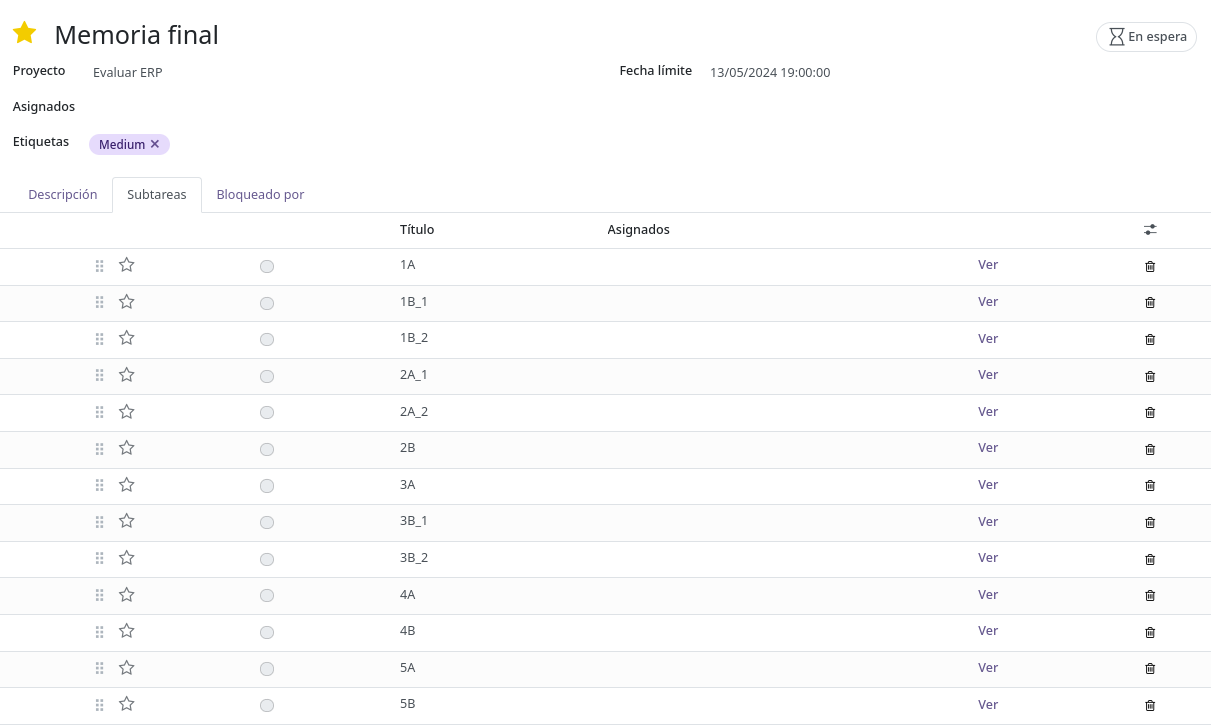
\includegraphics[width=0.75\linewidth]{tareaMemoria.png}
    \caption{Vista de una tarea}
\end{figure}
\paragraph{}
El flujo de trabajo de un equipo de trabajo que tiene un líder y trabajadores es diferente al que nosotros hemos realizado. Este flujo se basaría en que el líder define las tareas y las añade al tablero. Añade los datos pertinentes a la tarea y se la asigna a un miembro del equipo. Esta persona, cuando vea que se le ha asignado una tarea, la moverá a la columna de \textit{En proceso} y se pondrá a realizarla. Una vez que la haya acabado, cambiará el estado de la tarea a \textit{Hecho} y esperará a que se le asigne una nueva tarea. El flujo de trabajo descrito se ve reflejado en el diagrama BPMN (ver Figura \ref{fig:BMMN_trabajo}). 

\begin{figure}[h]
    \centering
    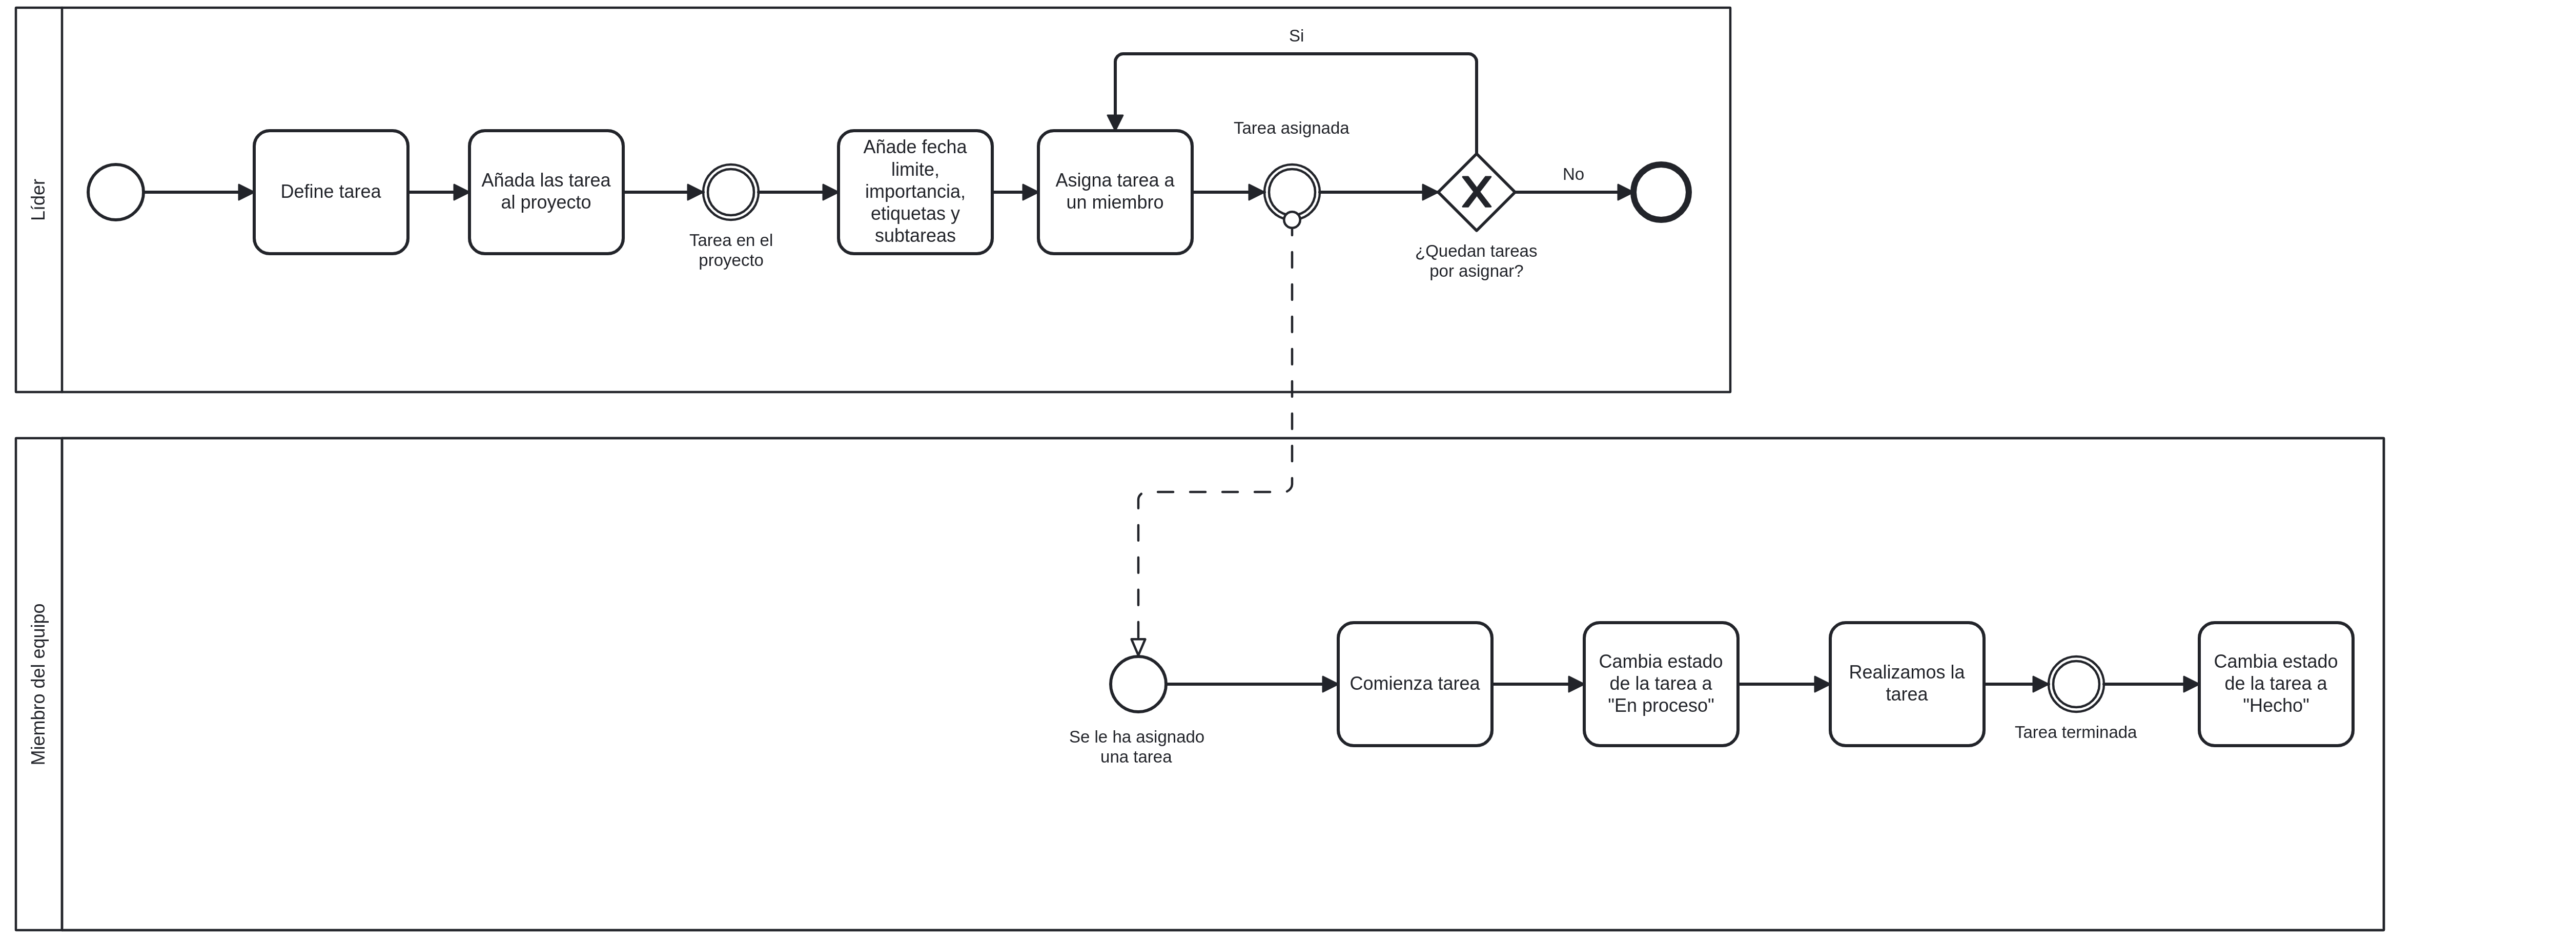
\includegraphics[width=1\linewidth]{ProjectsBPMN.png}
    \caption{Diagrama BPMN del flujo de trabajo de una empresa}
    \label{fig:BMMN_trabajo}
\end{figure}
\paragraph{}
Nuestro flujo de trabajo no ha sido como este; se basaba en cada día que hemos trabajado en el proyecto, lo primero que hacíamos era abrir este módulo y ver el estado global de este mediante la vista Kanban. Si en la columna \textit{En proceso} se encontraba alguna tarea, continuábamos con ella; si, por el contrario, estaba vacía, seleccionábamos una nueva tarea. En el momento en que hemos acabado con todas las tareas, hemos comenzado a realizar la memoria, tarea que en el tablero estaba bloqueada por el resto de tareas. Con este diagrama BPMN se refleja nuestro flujo.

\begin{figure}[h]
    \centering
    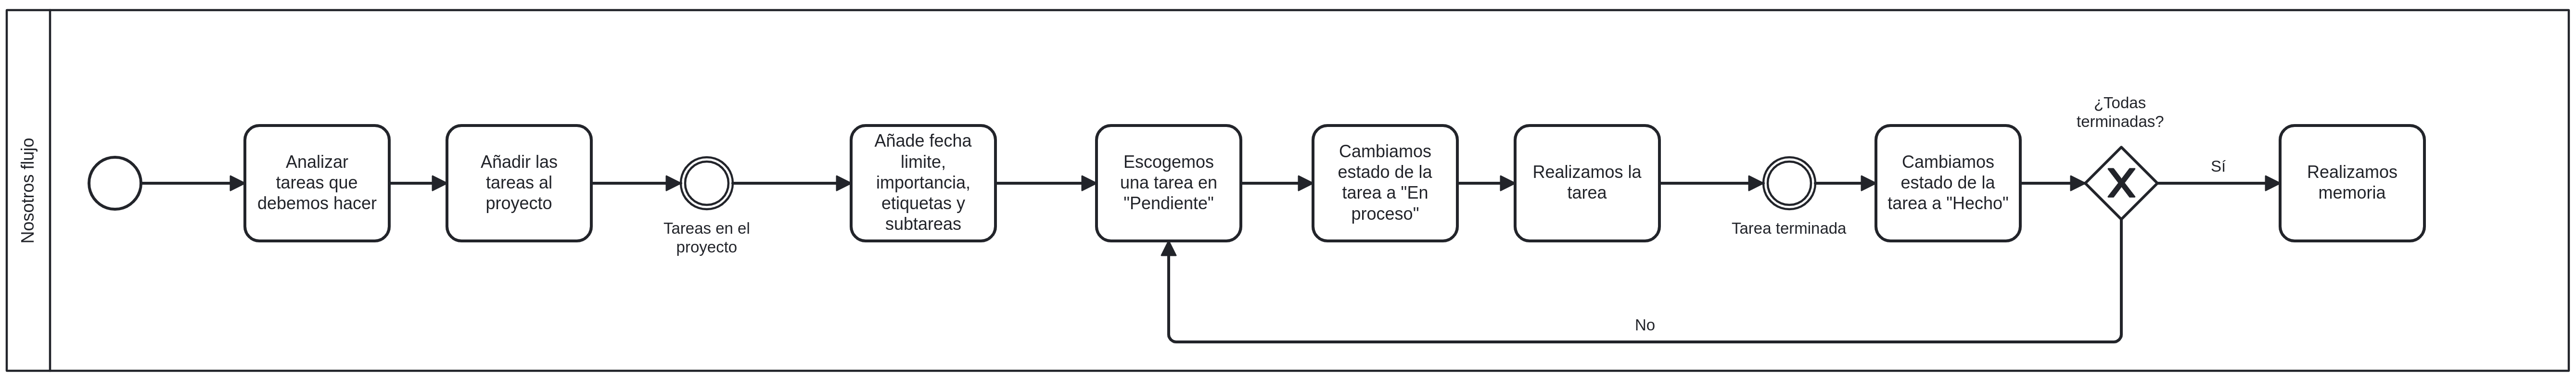
\includegraphics[width=1\linewidth]{ProjectsBPMN_2.png}
    \caption{Diagrama BPMN de nuestro flujo de trabajo}
\end{figure}
\paragraph{}
Bien es cierto que esta regla no se ha llevado a raja tabla, ya que ha habido ocasiones que había tareas en la segunda columna y escogíamos una nueva tarea. Estas decisiones siempre se han tomado de forma consensuada y fundamentada. Estas decisiones se han basado en bloqueos o porque las subtareas que faltaban eran para obtener la máxima nota.

\subsection{Conclusiones}
\paragraph{}
Tras haber trabajado con este módulo, consideramos que es uno de los mejores módulos que proporciona Odoo. Es intuitivo, fácil de usar y muy útil. Nos ha permitido llevar control en todo momento del estado de nuestro trabajo y saber qué tarea debíamos hacer en cada momento. Además, su vista Kanban permite cambiar el estado de las tareas de una forma cómoda y rápida. Esta vista se asemeja mucho a los tablones de tarjetas que se utilizan normalmente, permitiendo que desde cualquier lugar se pueda modificar y no sea necesario estar de forma presencial.
\paragraph{}
Creemos que no hemos llegado a exprimir todo su potencial al no haber utilizado la asignación de tareas. Realizando un análisis de nuestra organización en este proyecto, consideramos que podría haber sido mucho mejor, desde dividir las tareas a realizar el trabajo de forma más constante y no dejando gran parte de las tareas para las últimas semanas. Por último, ha habido tareas que se deberían haber realizado desde el principio como la instalación de Odoo en una máquina remota y la realización de backups diarias. Esto nos hubiera ahorrado muchos problemas y facilitado el trabajo.

\paragraph{}
En resumen, el módulo de gestión de proyectos de Odoo ha sido una herramienta invaluable para nuestro equipo, proporcionando una base sólida para la colaboración y el seguimiento del progreso del proyecto. Al reflexionar sobre nuestra experiencia, reconocemos las áreas de mejora y nos comprometemos a aplicar estas lecciones en proyectos futuros para lograr resultados aún más exitosos.

\newpage


\section{Gestión de la fabricación}
\subsection{Autoevaluación}
En esta sección se ha cumplido los objetivos correspondientes al 10.
\subsection{Introducción}
\paragraph{}
La gestión de fabricación es una parte importante en el proceso de producción de las empresas, y Odoo ofrece un conjunto de módulos diseñados para gestionarlo. Odoo nos permite programar y controlar el proceso de fabricación de productos. Además, facilita el seguimiento y la gestión de los movimientos de inventario, la recepción de materias primas, el almacenamiento de productos en almacenes y permite la gestión de todo el proceso de las compras.
\subsection{Metodología}
\paragraph{}
Para llevar a cabo la gestión de la fabricación en Odoo, se ha instalado los módulos de \textit{Fabricación}, \textit{Inventario} y \textit{Compras}. A continuación, se han realizado cambios en los ajustes para adaptar estos módulos a nuestras necesidades. Se ha activado en ajustes del módulo Inventario la opción \textit{Ubicaciones de almacenamiento} y \textit{Rutas multietapa} y en el módulo de Fabricación se ha activado la opción \textit{Ordenes de trabajo}. 
\paragraph{}
La empresa CochesMA se ocupa de la venta de vehículos. Para ello, desde el módulo de Fabricación y en el menú de Productos se ha creado un producto llamado Coche Mini completando la información referente al producto y este producto solo puede ser vendido y se obtendrá mediante su fabricación. Los otros 3 productos también se han creado pero en este caso solo pueden ser comprados y se obtendrán mediante la compra. A continuación, en el menú de lista de materiales se crea una nueva entrada donde se ha definido que el coche se fabricará con los siguientes productos: 4 \textit{Ruedas}, un \textit{Motor} y un \textit{Chasis}. 
\paragraph{}
Para probar que se ha puede realizar la fabricación manual de un producto, primero se ha comprado la cantidad necesaria de los tres productos desde el menú \textit{A mano} dentro de cada producto, actualizando su cantidad. Tras esto, desde el producto del Coche Mini se hace click en reponer y como consecuencia se habrá generado una orden de fabricación. Si se accede a esta orden y se confirma esta operación, se puede ver que la lista de productos se ha generado un coche y se han consumido los materiales necesarios para su fabricación. 
\paragraph{}
También, se pueden distribuir los productos y materiales en distintos almacenes, para probarlo se han creado 2 almacenes nuevos. De esta manera tenemos el almacén principal \textit{CochesMA} y los dos nuevos, \textit{CochesMA - almacén 2} y \textit{CochesMA - almacén 3}. Se ha definido que se va a almacenar las ruedas en el almacén 2, los motores en el almacén 3 y tanto los coches fabricados como los chasis en el almacén principal. Cuando se necesite realizar la fabricación de un coche las ruedas y los motores necesarios se trasladarán al almacén principal donde junto al chasis se procederá a fabricar el coche. Además, se ha automatizado la acción de comprar los productos cuando se acaben y de trasladarlos al almacen principal para su fabricación. Para ello, se han utilizado las reglas de reabastecimiento de la siguiente manera:
\begin{figure}[h]
    \centering
    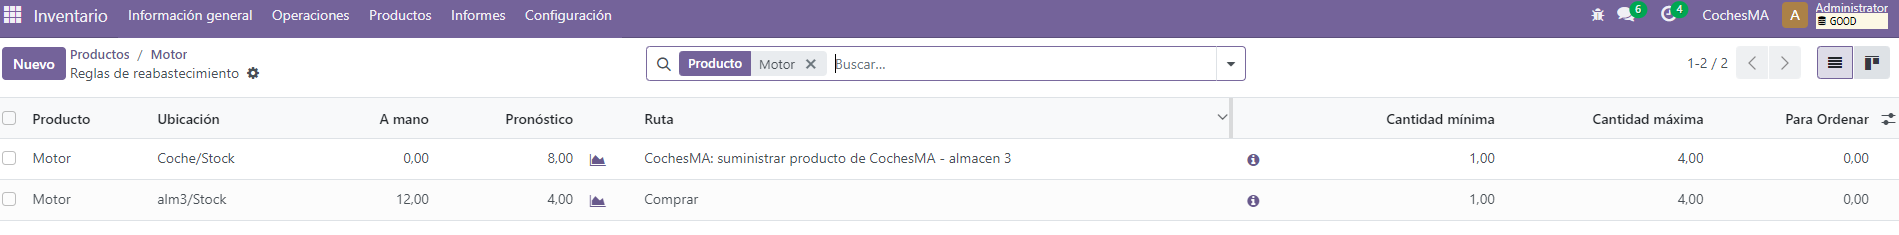
\includegraphics[width=1\linewidth]{fotosGestFab/ruedas.png}
    \caption{Reglas de reabastecimiento de las ruedas}
    \label{fig:enter-label}
\end{figure}
\paragraph{}
También se ha automatizado la fabricación de los vehículos por lo que cuando haya un pedido de un vehículo si no hay existencias se comenzará con la fabricación del mismo. 
\subsection{Resultados y análisis}
\paragraph{}
En este apartado se ha evaluado la capacidad de gestionar la fabricación que ofrece Odoo mediante los módulos de Fabricación, Inventario y Compras. Se han hecho configuraciones para personalizar estos módulos a las necesidades de las pruebas que se querían realizar. Además, se ha creado el producto Coche Mini que tiene una lista de materiales con los que se fabricará, 4 ruedas, un chasis y un motor.
\begin{figure}[h]
    \centering
    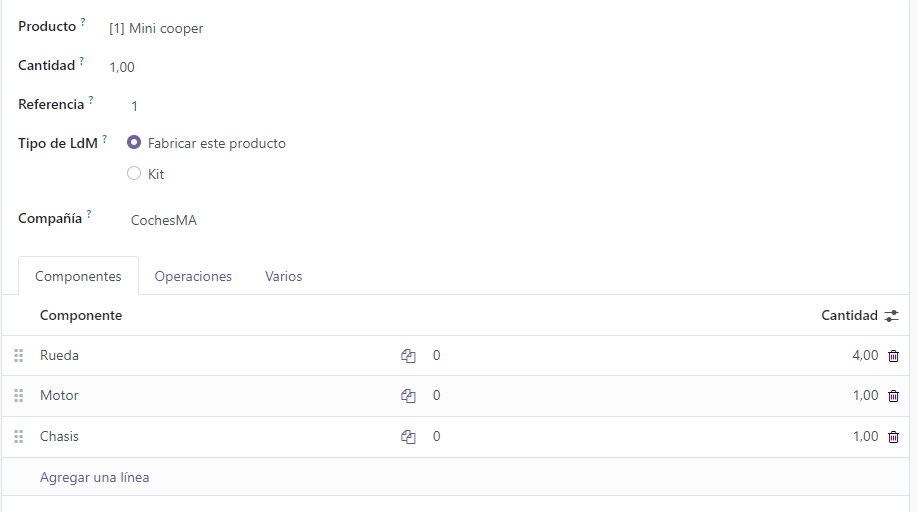
\includegraphics[width=1\linewidth]{fotosGestFab/coche.png}
    \caption{Lista de materiales de un coche Mini}
    \label{fig:enter-label}
\end{figure}
\paragraph{}
Se ha realizado la fabricación de un coche Mini de forma manual.
\begin{figure}[h]
    \centering
    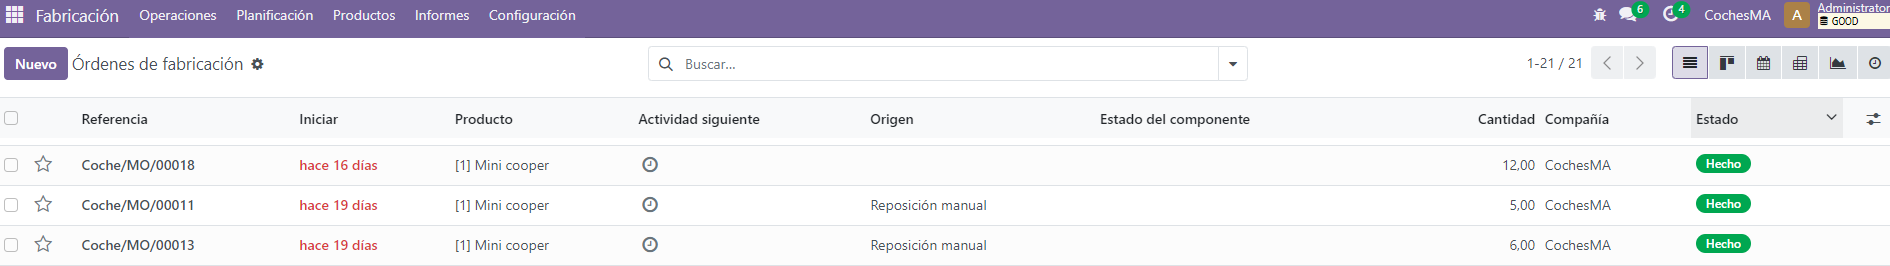
\includegraphics[width=1\linewidth]{fotosGestFab/manual.png}
    \caption{Orden de fabricación de un coche Mini de forma manual}
    \label{fig:enter-label}
\end{figure}
\paragraph{}
Por último, se ha automatizado la compra y transferencia de productos entre almacenes para cumplir con la producción necesaria.
\begin{figure}[h]
    \centering
    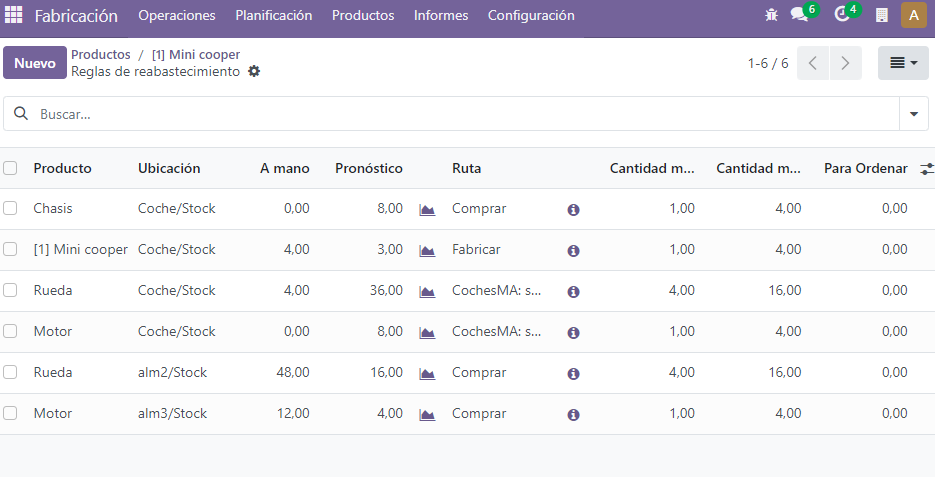
\includegraphics[width=1\linewidth]{fotosGestFab/reabastecimiento.png}
    \caption{Orden de reabastecimiento de los productos}
    \label{fig:enter-label}
\end{figure}
\paragraph{}
Por ultimo, se ha realizado un diagrama BPMN (figura \ref{fab}), el cual describe cómo se realiza el proceso de fabricación de un coche.
\begin{figure}[h]
    \centering
    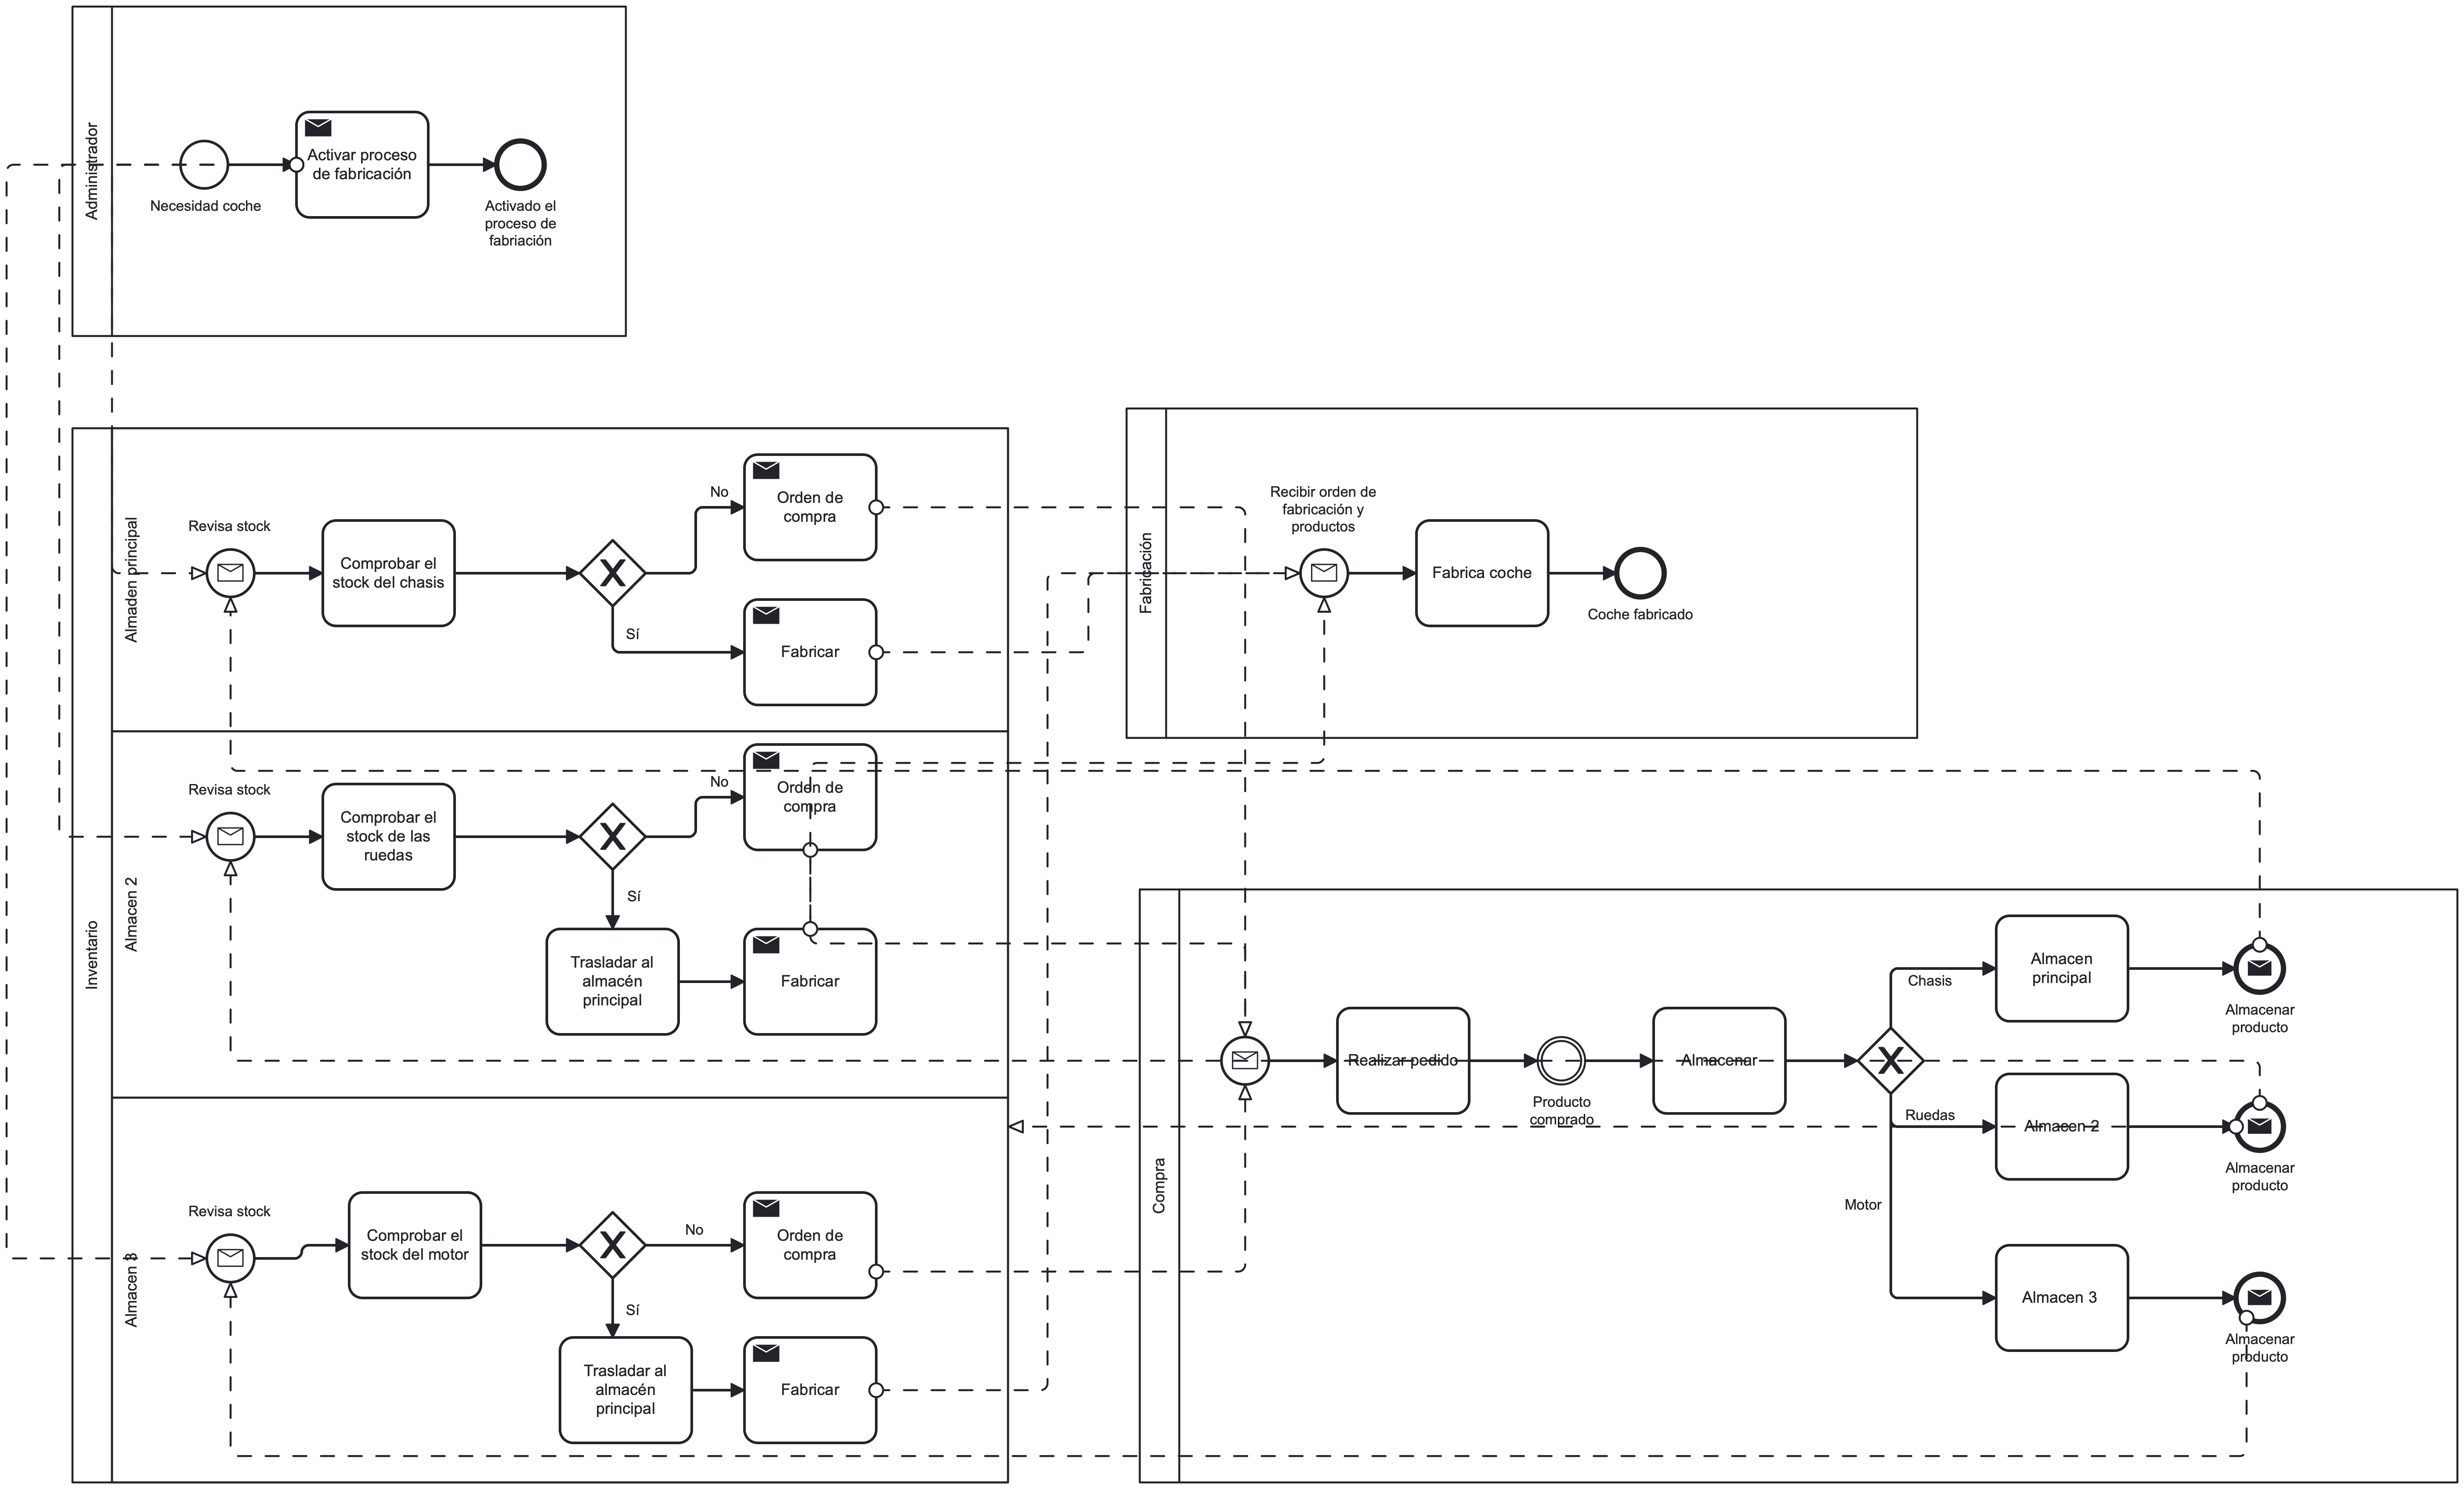
\includegraphics[width=1\linewidth]{fotosGestFab/Fabricacion.png}
    \caption{Diagrama BMPN 2.0 del proceso de fabricación}
    \label{fab}
\end{figure}
\subsection{Conclusiones}
\paragraph{}
La gestión de la fabricación en Odoo ofrece una gran cantidad de herramientas para controlar y optimizar el proceso de producción. Sin embargo, durante la realización de las pruebas y configuraciones, se han detectado tareas complejas como la automatización de las reglas de abastecimiento. Además, puede ser dificil de configurar correctamente para usuarios novatos porque el proceso de gestión de almacenamientos puede resultar confusa. Se recomienda proporcionar una formación adecuada a los empleados que se dediquen a este sector ya que es complicado de gestionar pero Odoo ofrece unas funcionalidades con un gran potencial, que permitirá optimizar en tiempo la gestión de los productos, su fabricación y su ubicación.
\newpage

\section{Relación con los clientes}
\subsection{Autoevaluación}
En esta sección se han cumplido los objetivos correspondientes al 10.
\subsection{Introducción}
\paragraph{}
En este apartado se va a realizar una gestión de las relaciones con los clientes en Odoo. Este factor es determinante para el éxito y la competitividad de la compañía. Se ofrecen varias herramientas y módulos dirigidos a la relación con los clientes que proporcionan la capacidad de captar, gestionar y cerrar acuerdos con clientes de manera eficiente. Se tiene como objetivo evaluar la idoneidad de Odoo como plataforma para este tipo de gestión.
\subsection{Metodología}
\paragraph{}
Para llevar a cabo la evaluación de esta sección se ha instalado los módulos CRM, Ventas y Facturación. A continuación, se han configurado estos módulos. Se ha activado la opción \textit{Leads} en los ajustes del módulo \textit{CRM}. Se ha establecido como divisa principal el Euro en los ajustes del módulo de Facturación.
\paragraph{}
El primer paso ha sido crear un equipo de ventas, para ello, se ha ido al módulo de ventas y se ha seleccionado la opción de \textit{Equipos de ventas}. Se ha creado un equipo de ventas llamado España que está formado por el usuario Pedro y James y tiene como líder del equipo a John. 
\paragraph{}
Por otro lado, se han creado 3 empresas cliente. Desde el módulo de ventas se ha hecho clic en el desplegable de pedidos y se ha seleccionado Clientes. Se ha creado la empresa cliente de origen español Zara, la cual durante el proceso de creación se han añadido 2 contactos en el apartado de Contactos y direcciones, Maria y Miguel. También, se ha creado el cliente Mercadona de origen español y se han añadido Pedro y Lucia como contactos de la empresa. Por otro lado, de origen suizo se ha creado como cliente la empresa de Nestle con los contactos de Theo y Francois. 
\paragraph{}
Durante el proceso de creación de cada empresa cliente se ha completado el campo de Condiciones de pago que se ubica en el panel de Venta y compra, en las empresas españolas se paga a 30 días  y las empresas suizas se paga a 45 días. En el mismo panel se ha asignado la Tarifa de las empresas españolas en Euros, mientras que en la empresa suiza se ha creado una nueva tarifa para que la lista de precios esté en Francos Suizos.
\paragraph{}
Desde la compañía nos hemos puesto en contacto con los clientes ofreciendo nuestro producto y como resultado, Mercadona y Zara se han mostrado interesados por lo que se han creado 2 iniciativas, una cada una de las empresas cliente. Para ello, desde el módulo \textit{CRM} en el menú de \textit{Leads} se han creado 2 entradas. Cada una se ha asignado a uno de los contactos de la empresa correspondiente y se ha establecido el ingreso esperado y la probabilidad que existe de que se convierta en oportunidad.
Además, desde la vista de Kanban del módulo de CRM se puede observar que se han añadido dos entradas en el apartado de nuevo.
\paragraph{}
La empresa de Mercadona nos ha pedido una reunión para la semana siguiente por lo que el lead se ha convertido en una oportunidad, para ello se ha hecho clic en Convertir a oportunidad desde el lead correspondiente y se ha asignado al usuario Pedro como comercial y al equipo de ventas \textit{Ventas}. Además, desde el apartado de reuniones de la oportunidad se ha configurado una reunión se ha añadido al calendario una reunión para el 1 de mayo de 2024 de 9:00 a 10:00 con Lucía que es el contacto de Mercadona.
\paragraph{}
Tras la reunión, nos ha pedido que le enviemos un presupuesto para ello, desde la vista de la oportunidad se ha hecho clic en Nuevo presupuesto. Se ha creado un presupuesto con la información correspondiente y se le ha enviado por correo, pasando la venta al estado de Calificado y a Propuesta arrastrando la venta de un estado a otro. El cliente tras examinarlo nos ha pedido una reducción de un 5\% de descuento, para ello hemos tenido que activar la opción de Descuentos en los ajustes del módulo de Ventas. De esta manera se ha podido agregar un descuento del 5\% al presupuesto y se lo hemos vuelto a enviar al cliente. Finalmente, el cliente confirma el segundo presupuestos y se cierra el acuerdo, pasando la venta al estado de Ganado.
\newpage
\subsection{Resultados y análisis}
\paragraph{}
Durante este apartado se ha realizado la configuración de los módulos de Odoo necesarios para la gestión la relación de los clientes y las ventas. Se ha simulado un proceso de venta de un coche Mini que ha sido ofrecido a varios clientes.
\begin{figure}[h]
    \centering
    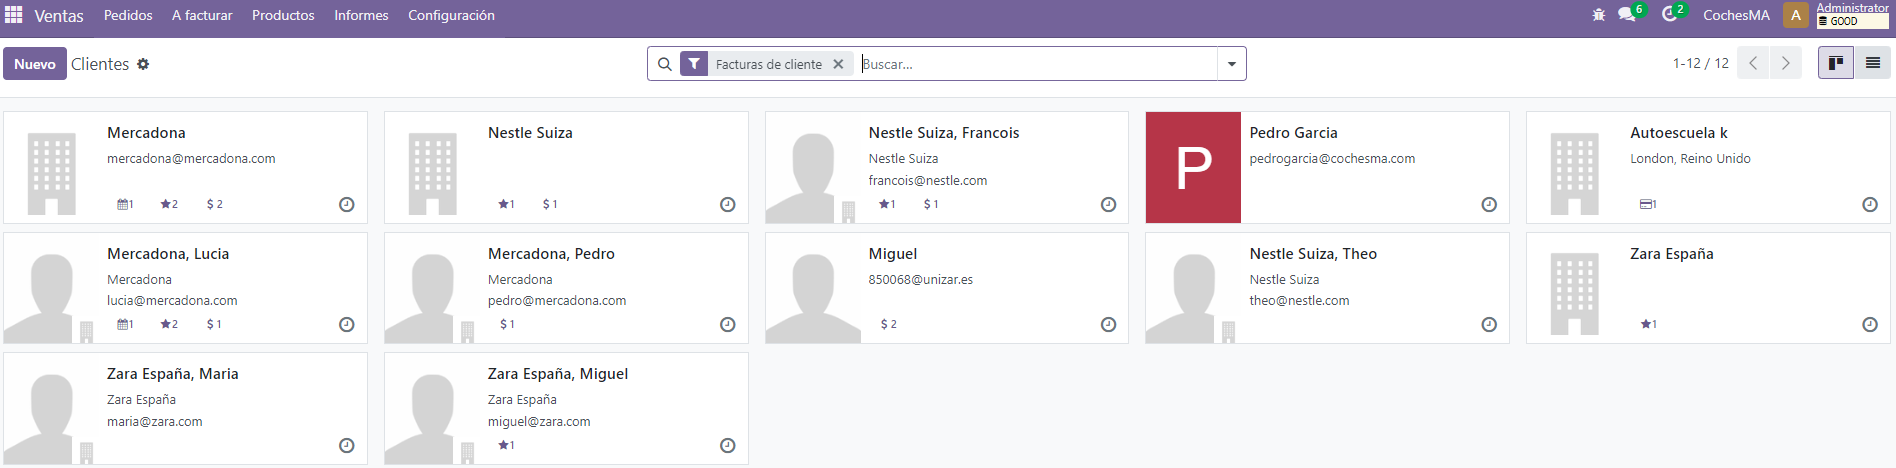
\includegraphics[width=1\linewidth]{fotosRelacion/clientes.png}
    \caption{Lista de clientes de la compañía con sus respectivos contactos}
    \label{fig:enter-label}
\end{figure}
\paragraph{}    
En este proceso se han creado 2 iniciativas para dos clientes interesados. Se ha creado un presupuesto para uno de ellos. Finalmente, en una segunda revisión del presupuesto se ha aplicado un descuento del 5\% de descuento sobre el precio y se ha cerrado el acuerdo de venta.
\begin{figure}[h]
    \centering
    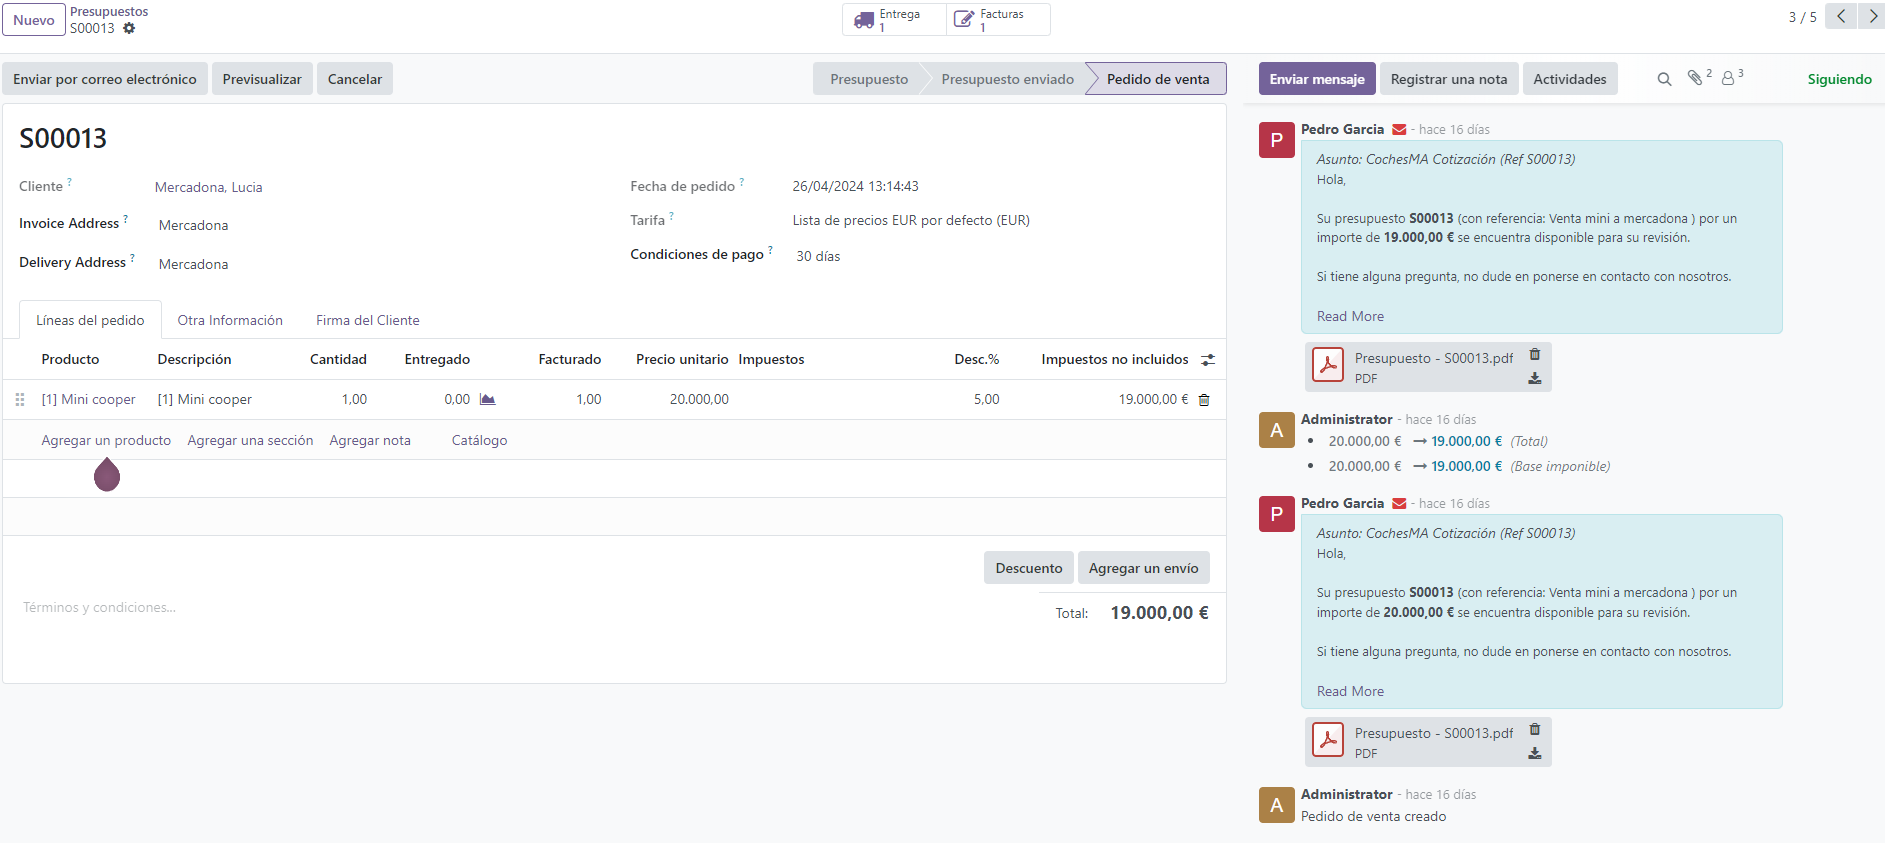
\includegraphics[width=1\linewidth]{fotosRelacion/presupuesto.png}
    \caption{Presupuesto de la venta}
    \label{fig:enter-label}
\end{figure}
Este proceso también está sincronizado con el módulo de Facturación por lo que el estado de la venta se puede observar desde la siguiente vista.
\newpage
\begin{figure}[h]
    \centering
    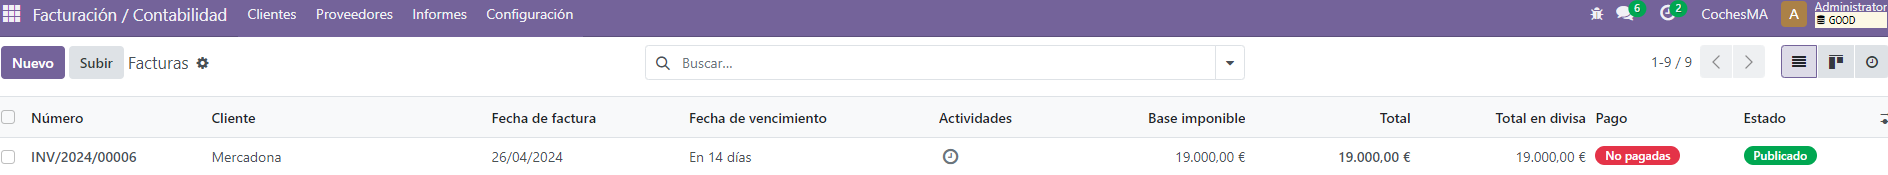
\includegraphics[width=1\linewidth]{fotosRelacion/facturacion.png}
    \caption{Lista de las ventas desde el módulo de Facturación}
    \label{fig:enter-label}
\end{figure}
Durante todo el proceso de venta se ha ido actualizando la vista Kanban del módulo \textit{CRM} que permite una vista general del estado de las iniciativas y ventas.
\begin{figure}[h]
    \centering
    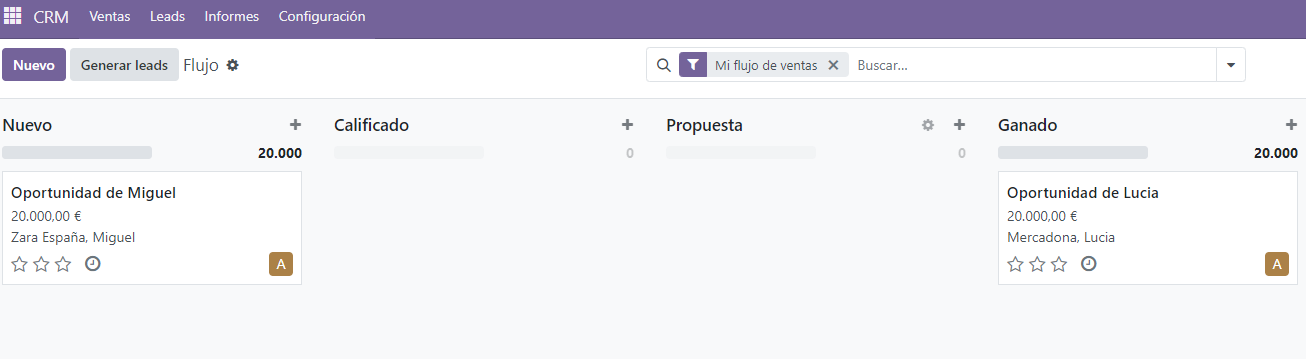
\includegraphics[width=1\linewidth]{fotosRelacion/kanban.png}
    \caption{Vista Kanban del flujo de ventas del módulo CRM}
    \label{fig:enter-label}
\end{figure}
Por último, se ha realiza un BPMN sobre el proceso de venta.
\begin{figure}[h]
    \centering
    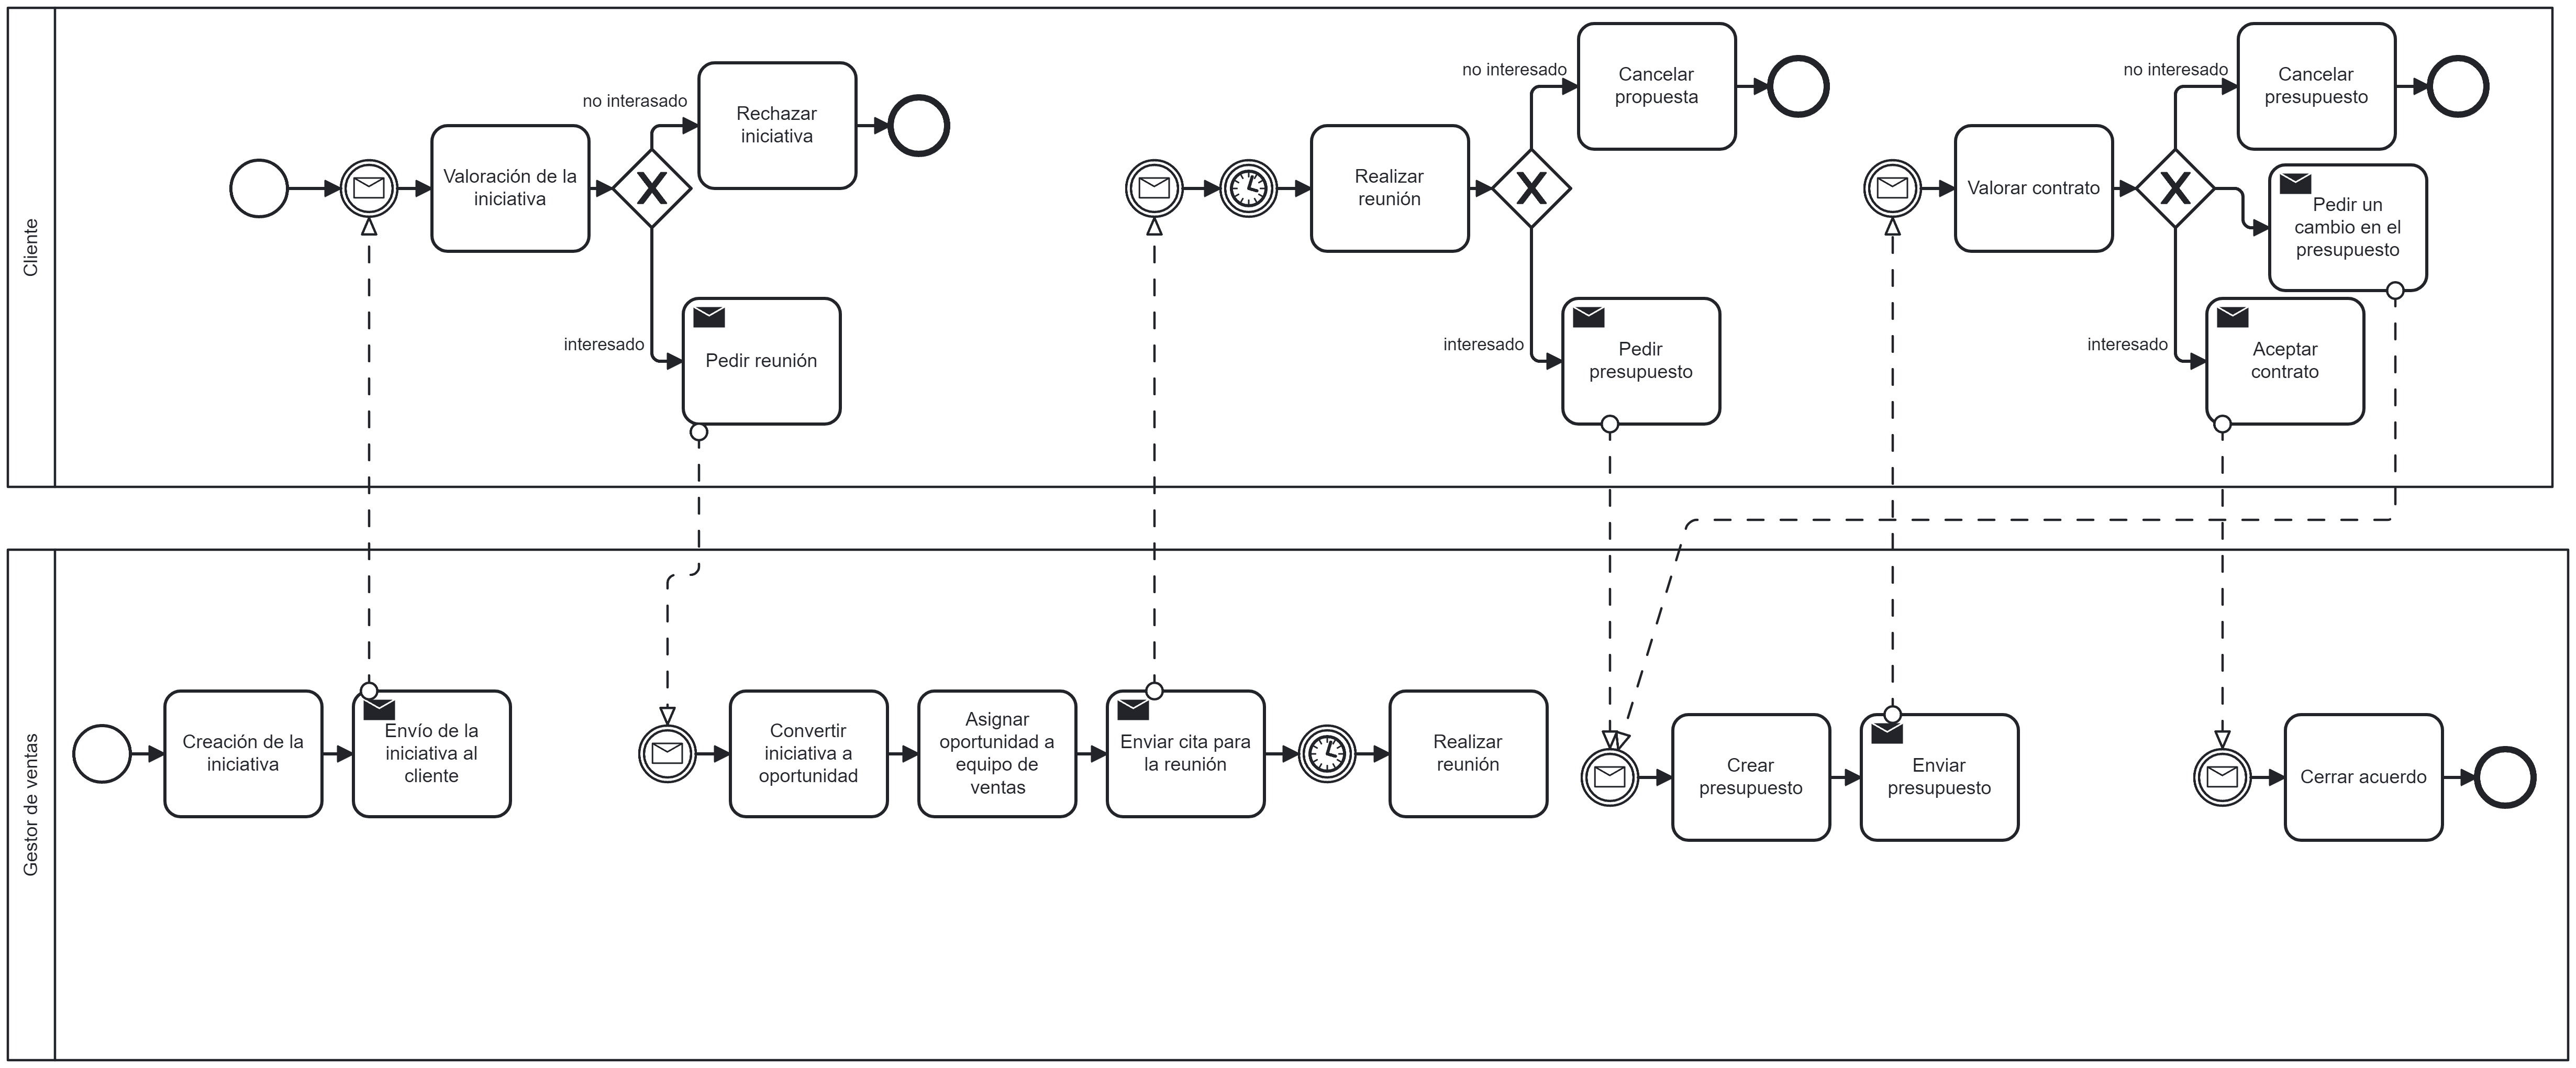
\includegraphics[width=1\linewidth]{bpmn/venta.png}
    \caption{BPMN del proceso de venta}
    \label{fig:enter-label}
\end{figure}
\subsection{Conclusiones}
\paragraph{}
La solución que ofrece Odoo para estas funcionalidades las cubre mediante el módulo \textit{CRM}, \textit{Ventas} y \textit{Facturación}. De esta manera se permite gestionar de manera eficiente la relación con los clientes y gestionar el proceso de ventas y facturación. La configuración de estos módulos es relativamente simple, y una vez realizado, proporciona una plataforma sólida para cubrir la gestión de clientes, oportunidades de negocio, presupuestos y facturas.
\paragraph{}
Se ha demostrado como se ha utilizado de forma efectiva las herramientas disponibles para llevar a cabo la generación de leads, la creación de presupuestos y facturas mediante Odoo. Además, gracias a la integración del correo electrónico en la sección de Configuración técnica se facilita la comunicación con los clientes y la transferencia de presupuestos y facturas.
\paragraph{}
En este apartado se ha evaluado la capacidad de Odoo para la gestión de relaciones con los clientes y las ventas. Se ha confirmado que Odoo ofrece una plataforma completa para llevar a cabo esta gestión, permite una configuración flexible y capacidad para optimizar la gestión comercial de la compañía. En resumen, tiene una correcta implementación de módulos para llevar a cabo la relación con los clientes y desarrollar los procesos de venta mediante Odoo. 
\newpage

\section{Gestión de Personal}
\subsection{Autoevaluación}
En esta sección se han cumplido los objetivos correspondientes al 10.
\subsection{Introducción}
\paragraph{}
En cuanto a la gestión de recursos humanos Odoo ofrece un conjunto de módulos que incluyen herramientas para su realización. En ella se engloba los procesos de reclutamiento y de la gestión del personal una vez que han sido contratados. De esta manera permite a las organizaciones gestionar eficientemente el reclutamiento para cada etapa del proceso, definir criterios de evaluación y mantener un registro de los postulantes. Por otro lado, gestiona la información de los empleados, evaluar su desempeño y asignar responsabilidades.
\subsection{Metodología}
\paragraph{}
Para comprobar el funcionamiento de este aspecto en Odoo se ha instalado los módulos de \textit{Proceso de selección} y \textit{Empleados}. En el módulo de Empleados se han creado varios departamentos desde el menú de departamentos, en la empresa raíz CochesMA se ha creado un departamento de Administración, Ventas y Servicios profesionales, en la rama de CochesMA.UK se ha creado un departamento de Gestión y otro de Ventas y en la rama de CochesMA.US se ha creado uno uno de Personal y otro de Servicios profesionales. Para cada uno durante la creación del mismo se ha asignado un gerente de entre las personas que se han creado en la sección de configuración funcional.
\paragraph{}
Además, dentro del menú configuración del módulo \textit{Empleados} se puede acceder al menú \textit{Puestos de trabajo}. Desde aquí se pueden crear puestos de trabajo rellenando la información necesaria en el formulario de creación, en este caso se ha creado dos director técnico, dos responsables de comunicación y ventas, dos gestores de personal, dos directores ejecutivos  y un consultor asignando cada uno a la empresa raíz o a una de las ramas. 
\paragraph{}
En cuanto al proceso de reclutamiento, vamos a simular una operación en el que se va a contratar a una persona para el departamento de \textit{Ventas} con al menos un año de experiencia en operaciones internacionales con suiza y que sepa Francés y Alemán. Para ello, se ha creado un nuevo puesto de trabajo Director de marketing como se ha explicado anteriormente y se añadido una descripción explicando en que consiste el puesto y los requisitos para ello. Además, desde el menú de Tipo de habilidad en el módulo de Reclutamiento se ha creado una entrada llamada \textit{Languages}, en el que se valoran idiomas como el Alemán, Francés, Inglés y Español, con niveles desde bajo, medio y avanzado. Por otro lado, también se ha creado un nuevo tipo de habilidad llamada experiencia la cual tiene como posibilidad operaciones internacionales con suiza, con distintos niveles según el tiempo de experiencia, 1, 2 o 3 años. También, se ha ido a configuración del módulo de Reclutamiento y se ha activado la opción de Pantalla de CV. Además, se ha definido un formulario de entrevista que tendrá que rellenar el candidato, para ello se ha hecho clic en los 3 puntos del puesto de trabajo en el módulo de reclutamiento y seleccionar la opción de Nuevo Formulario de entrevista y a continuación se ha rellenado con las siguientes 3 preguntas. Para que Odoo permita enviar el formulario creado se ha activado la opción de Enviar encuesta de entrevista en los ajustes del módulo.
\begin{figure}[h]
    \centering
    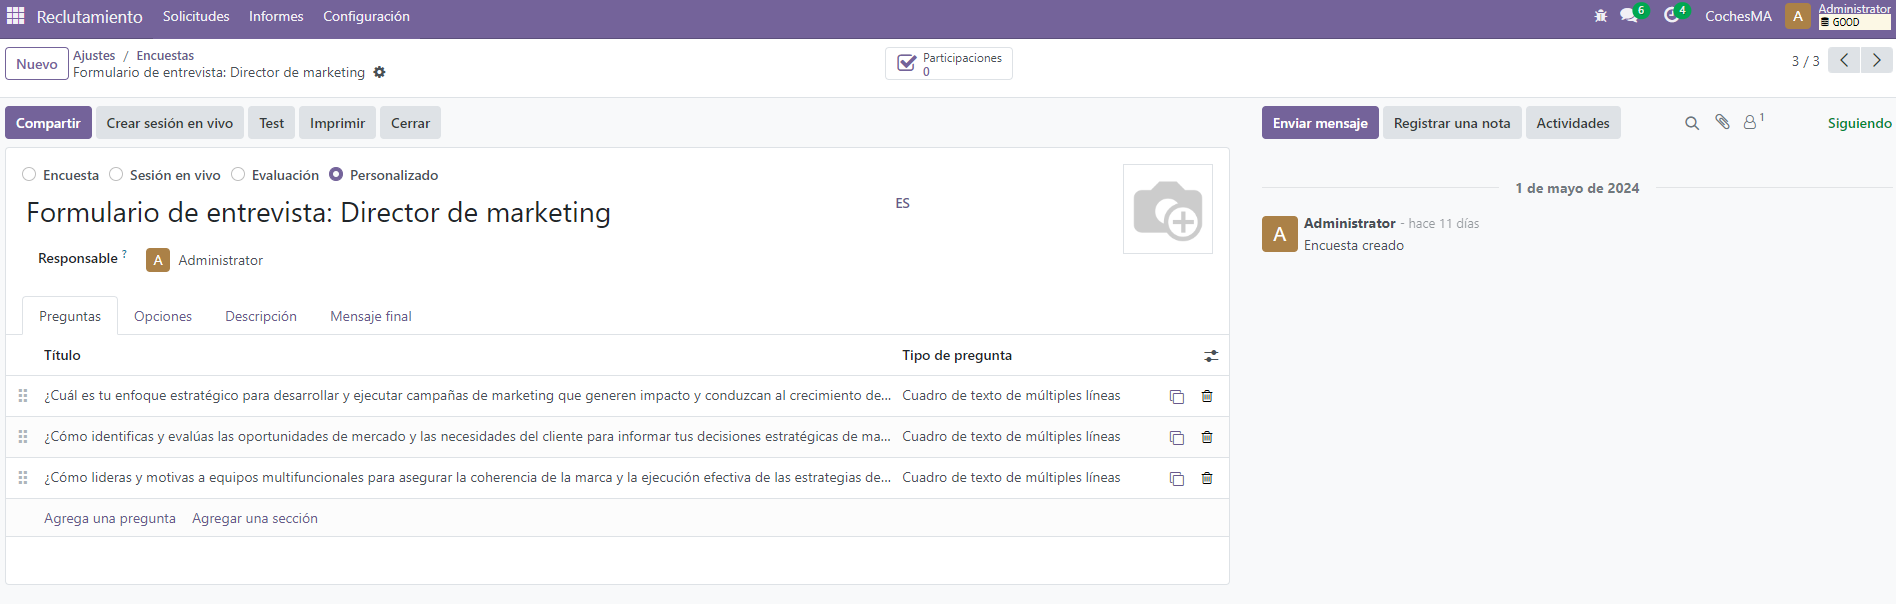
\includegraphics[width=1\linewidth]{fotosGestPers/image.png}
    \caption{Formulario de entrevista para el puesto de Director de marketing}
    \label{fig:enter-label}
\end{figure}
\paragraph{}
A continuación, en el modulo de reclutamiento se ha hecho clic al enlace Página de trabajos del puesto de Director de marketing. Se ha rellenado el formulario de la solicitud con la información correspondiente y se ha añadido el currículum y se ha enviado. Desde el módulo de Reclutamiento se ha podido ver la solicitud del puesto. Se ha hecho clic en él y se ha asignado en la opción de habilidades un nivel avanzado de Alemán y Francés y 1 año de experiencia en operaciones internacionales con suiza. Se ha realizado el proceso de reclutamiento con dos entrevistas se ha propuesto un contrato y se ha firmado. Finalmente, se ha creado un usuario de tipo empleado para el nuevo Director de marketing.
\subsection{Resultados y análisis}
\paragraph{}
Durante este apartado se ha creado en la compañía matriz un departamento de Administración, de Ventas y de Servicios profesionales, en la rama CochesMA.UK un departamento de Gestión y de Ventas y en la rama CochesMA.US un departamento de Personal y de Servicios profesionales. 
\begin{figure}[h]
    \centering
    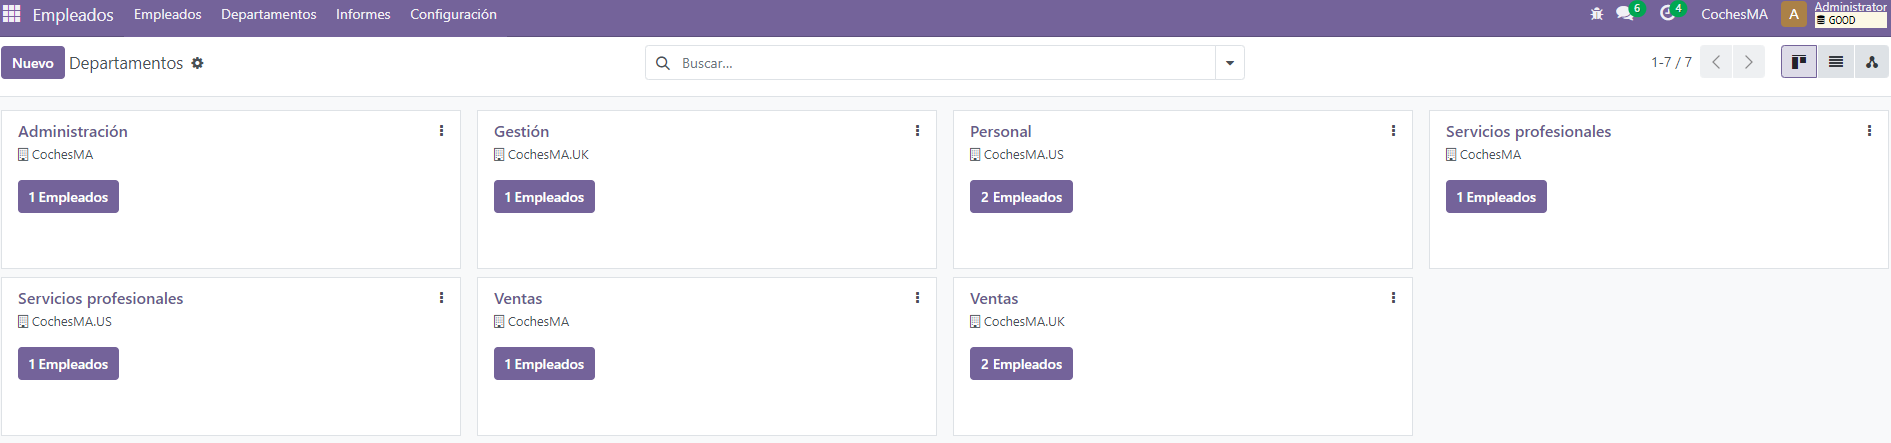
\includegraphics[width=1\linewidth]{fotosGestPers/departamentos.png}
    \caption{Lista de departamentos de la compañía}
    \label{fig:enter-label}
\end{figure}
\paragraph{}
Además, se han creado los siguientes puestos de trabajo dentro de cada departamento. Para el departamento de Administración un puesto de Director Ejecutivo, para el de Servicios profesionales un Director Técnico y un consultor, para el de Personal un Gestor de personal y para el Ventas un Responsable de comunicación y ventas. Se han creado 9 empleados, tantos como usuarios había y se han distribuido entre los puestos de trabajo. 
\begin{figure}[h]
    \centering
    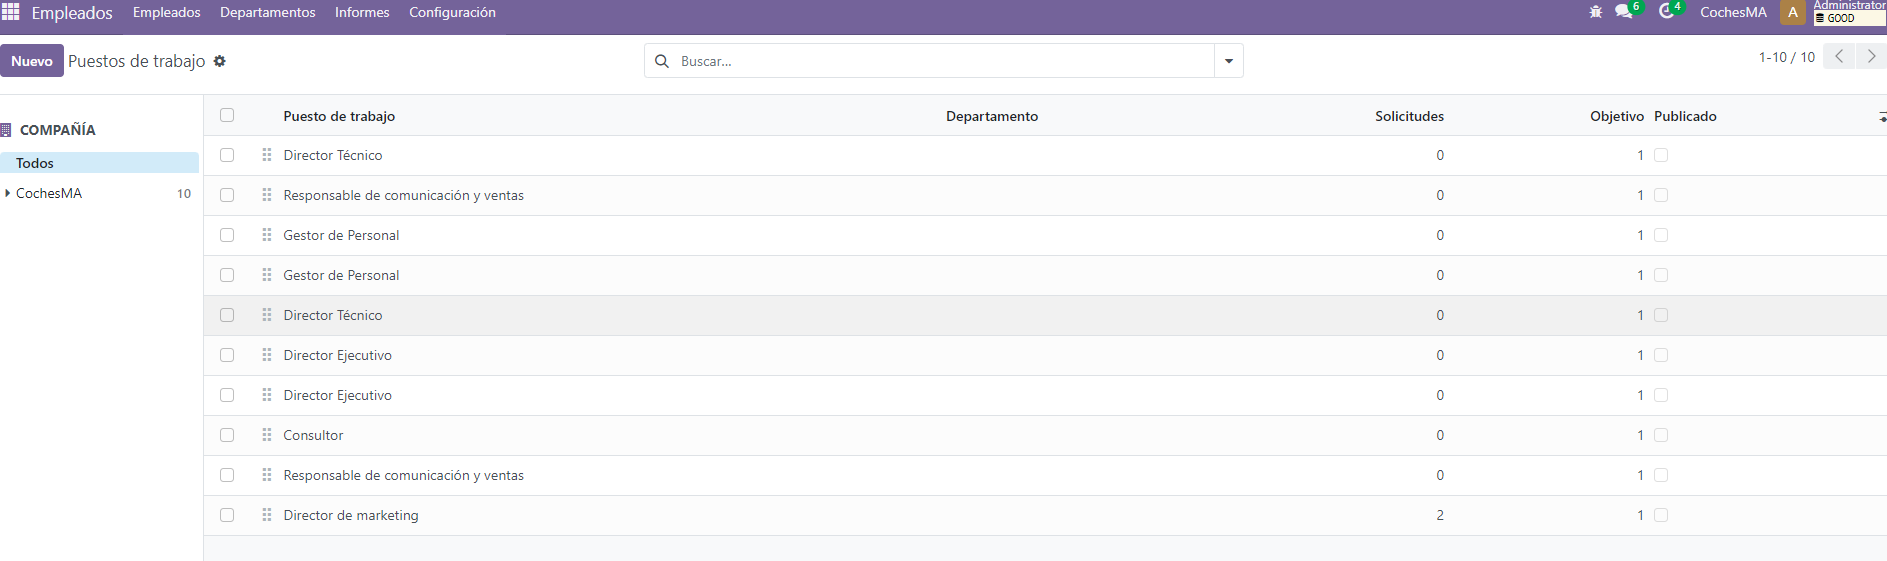
\includegraphics[width=1\linewidth]{fotosGestPers/puestos.png}
    \caption{Lista de departamentos de la compañía}
    \label{fig:enter-label}
\end{figure}
\begin{figure}[h]
    \centering
    
\includegraphics[width=1\linewidth]{fotosGestPers/empleados.png}
    \caption{Lista de empleados de la compañía}
    \label{fig:enter-label}
\end{figure}
\paragraph{}
Se ha creado un nuevo puesto de trabajo, Director de marketing y se ha simulado el proceso de reclutamiento y contratación de un nuevo empleado para este puesto utilizando la vista Kanban de solicitudes.
\begin{figure}[h]
    \centering
    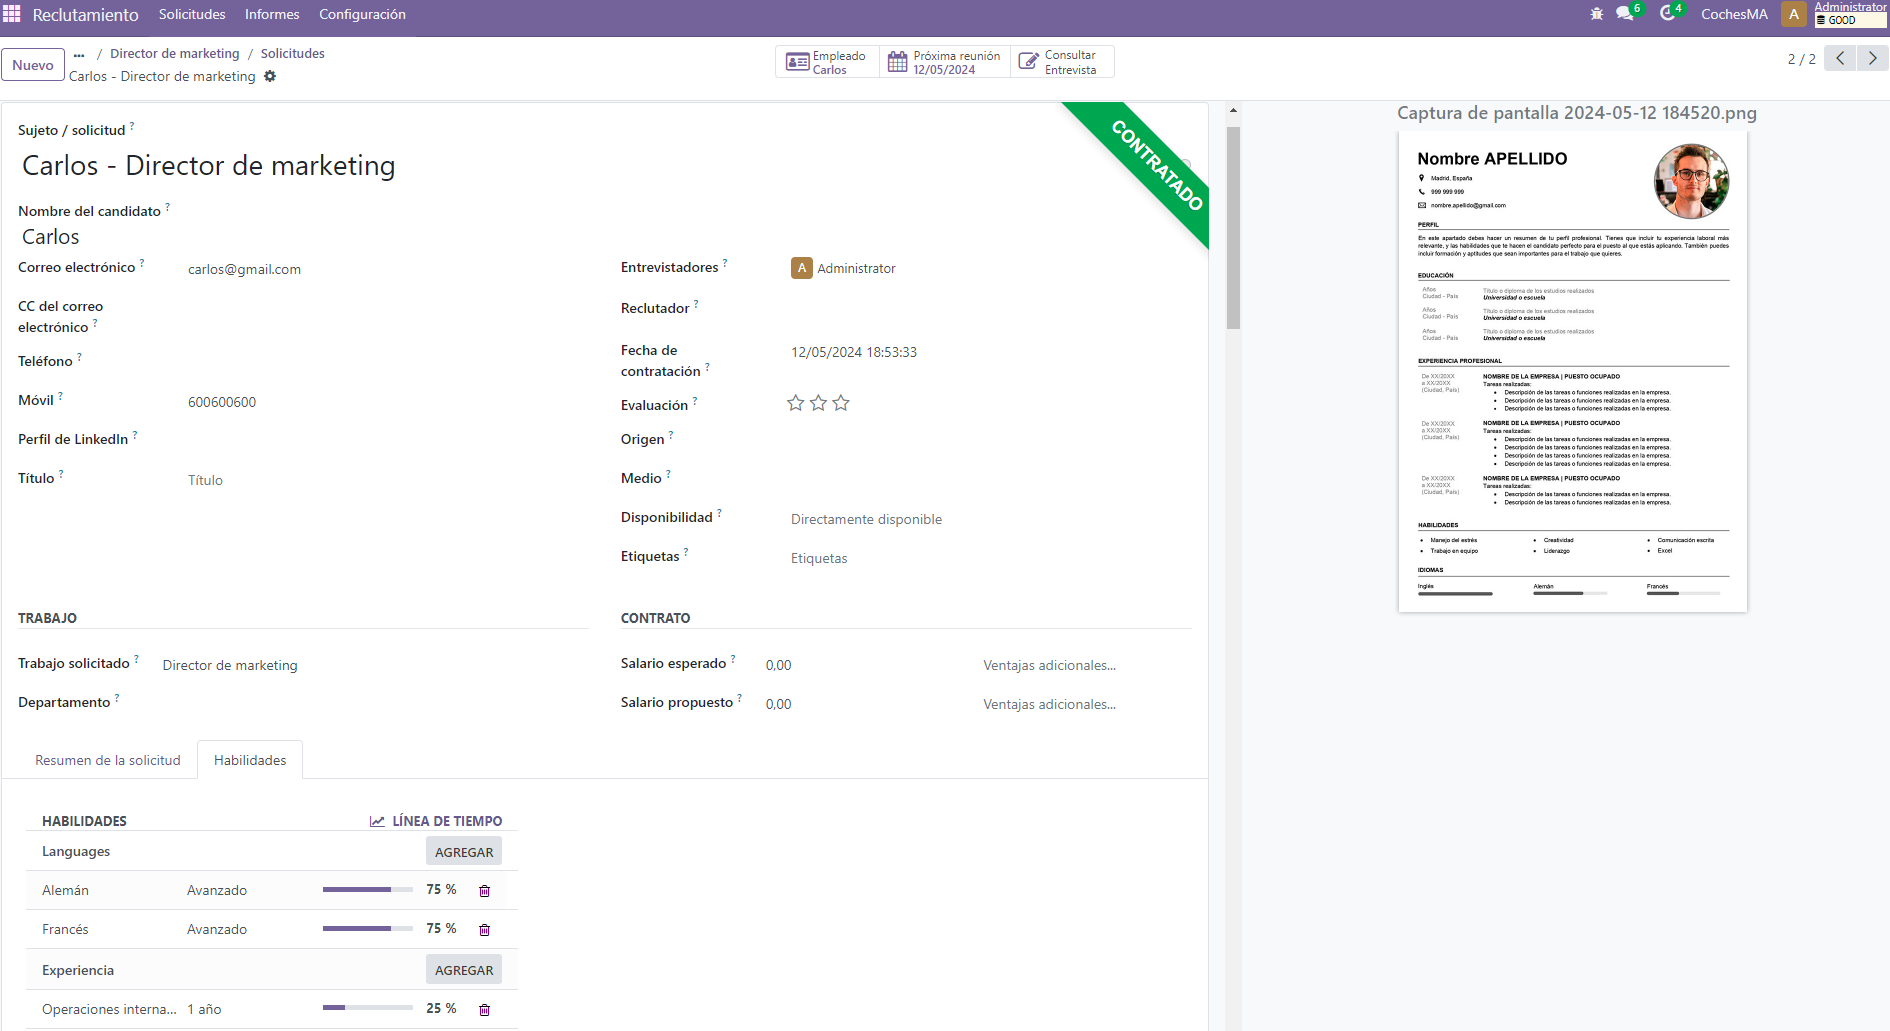
\includegraphics[width=1\linewidth]{fotosGestPers/reclutamiento.png}
    \caption{Solicitud al puesto de Director de marketing}
    \label{fig:enter-label}
\end{figure}
\begin{figure}[h]
    \centering
    
\includegraphics[width=1\linewidth]{fotosGestPers/kanban.png}
    \caption{Vista kanban con los candidatos y su estado en el proceso de reclutamiento}
    \label{fig:enter-label}
\end{figure}
\paragraph{}
Por último, se ha creado un BPMN del proceso de reclutamiento realizado.
\begin{figure}[h]
    \centering
    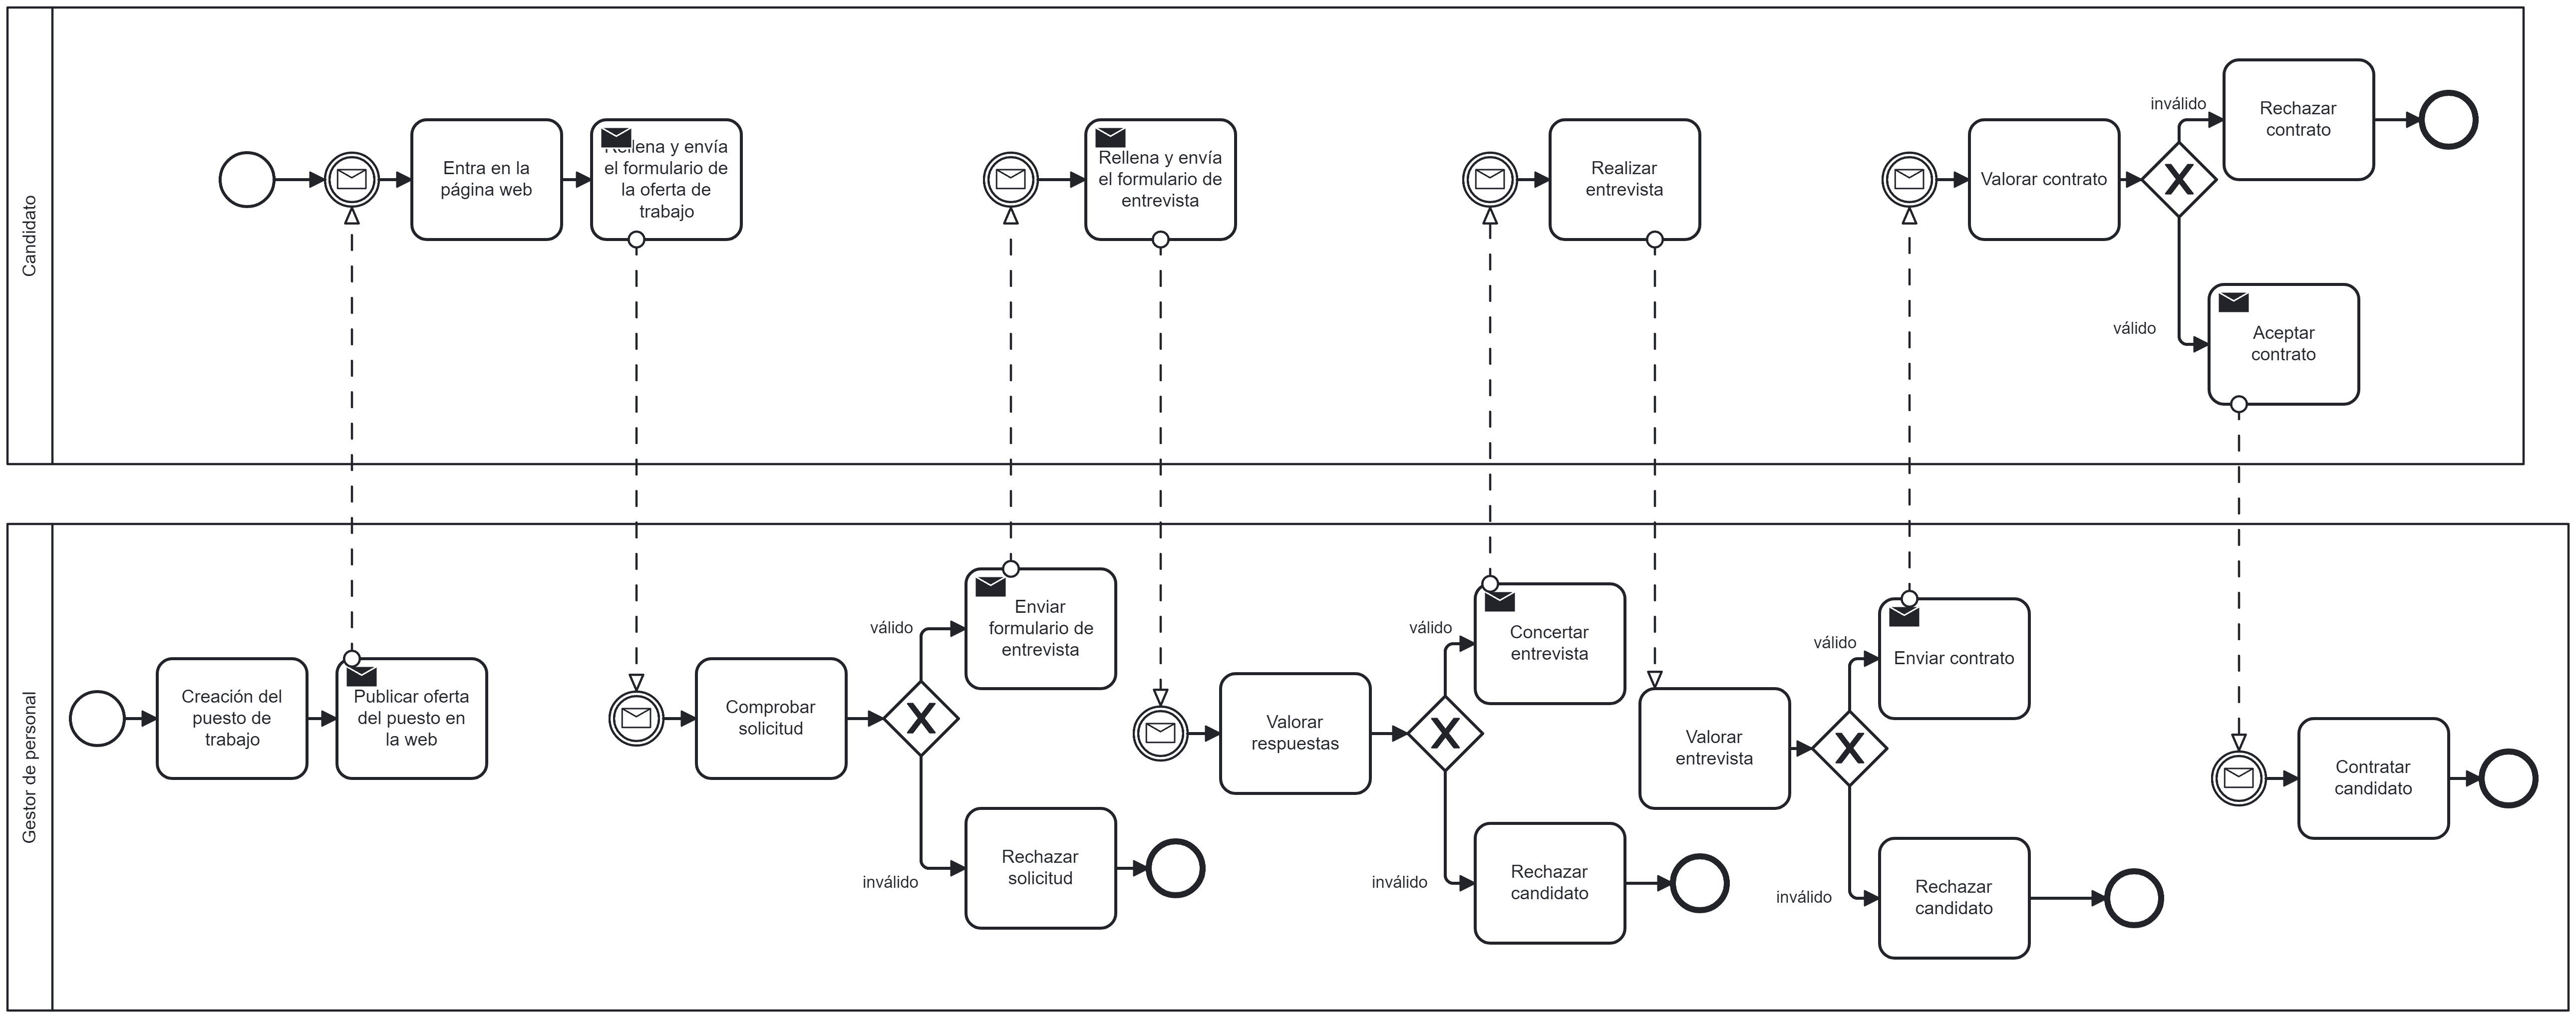
\includegraphics[width=1\linewidth]{bpmn/gestPers.png}
    \caption{Solicitud al puesto de Director de marketing}
    \label{fig:enter-label}
\end{figure}

\subsection{Conclusiones}
\paragraph{}
Durante la evaluación de la gestión de personal en Odoo, hemos observado que la parte relacionada con la creación de departamentos, puestos de trabajo y empleados se llevó a cabo de manera adecuada y eficiente. Se ha demostrado una comprensión clara de cómo configurar la estructura organizativa y asignar roles y responsabilidades dentro de la empresa. 
\paragraph{}
Sin embargo, en lo que respecta al reclutamiento y la gestión de solicitudes, hemos identificado algunos aspectos que requieren mejoras. Por ejemplo, hemos observado la necesidad de añadir manualmente desde Odoo las habilidades, experiencia y lenguaje del candidato, lo cual puede resultar poco práctico al no ser incluido directamente en el proceso de solicitud. Además, es importante tener en cuenta que la eficiencia de la gestión puede disminuir cuando se generan grandes cantidades de empleados.
\paragraph{}
A pesar de ello, es destacable que Odoo ofrece una plataforma sólida para la gestión de personal, con funcionalidades que incluyen diversas formas de evaluar el nivel del candidato, ya sea mediante entrevistas o formularios, lo cual resulta más eficiente.
\newpage

\section{Contabilidad y finanzas}
\subsection{Autoevaluación}
En esta sección se ha cumplido los objetivos correspondientes al 10.
\subsection{Introducción}
\paragraph{}
Uno de los módulos esenciales para cualquier empresa es el módulo de finanzas y contabilidad. Este debe de ayudar a sus usuarios a gestionar sus beneficios y gastos, además de encargarse de automatizar labores administrativos como la declaración de la renta o la gestión de impuestos. En esta sección se busca analizar el problema del módulo FICO de Odoo y buscar una solución, que nos permite gestionar la contabilidad y finanzas desde nuestro ERP. Para ello hemos realizado un estudio detallado sobre la gestión contable y financiera en Odoo, centrándose en el contexto español. Se identifican los problemas del módulo FICO en Odoo, se propone una solución en la nube y se describe el proceso de integración con Odoo. Este estudio tiene como objetivo proporcionar una visión integral de las opciones disponibles para las PYMEs españolas en términos de contabilidad y finanzas.
\subsection{Metodología}
\paragraph{}
La metodología empleada se basa en una revisión exhaustiva de los problemas reportados en el repositorio de Github \href{https://github.com/OCA/l10n-spain/issues}{OCA/l10n-spain issues}, así como en la evaluación de diversas soluciones FICO en la nube. Odoo es un software Open Source, por lo que gran parte de las mejoras son realizadas por la comunidad, como en este caso. Este repositorio es de la comunidad española de Odoo, la cual busca cada día mejorar este ERP. También, se ha realizado un análisis comparativo de las posibles soluciones encontradas; considerando sus características, ventajas y aplicabilidad a las necesidades específicas del mercado español. Por ultimo, se ha investigado como se puede llevar a cabo el proceso de integración entre Odoo y la solución FICO seleccionada, siguiendo pasos técnicos específicos.
\subsection{Resultados y análisis}
Tras analizar cual es el problema de este modulo nos hemos dado cuenta que existen varios problemas. El primer gran problema es que el soporte de este módulo en Odoo 17.0 es de pago además de estar incompleto. Otro gran problema es que si queremos utilizar Odoo en castellano muchas de sus funcionalidades no están migradas a este versión, por lo tanto, hay varios módulos que no se han implementado o están en proceso. Si queremos conocer cuales de los módulos son totalmente funcionales en la versión 17.0 podemos revisar el \textit{issue} del repositorio de Github \href{https://github.com/OCA/l10n-spain/issues/3298}{Migration to version 17.0}. Aquí encontraremos la información de los módulos que han sido migrados con éxito, cuales se está trabajando y cuales todavía no se pueden utilizar en castellano en la versión 17.0 de español. Analizando este lista podemos observar que a penas hay once ítems completados, de los 42 que se deben implementar. Otro problema que nos ha llamado la atención es el problema con las subvenciones. Un usuario de la comunidad ha creado un \textit{issue} reportando este problema. Sin embargo, el problema que más no ha llamado la atención es el problema con la \href{https://github.com/OCA/l10n-spain/issues/3527}{Gestión de IRPFs y sus posiciones fiscales}. En este \textit{issue} se describe el problema en la configuración de impuestos en Odoo. Actualmente no se garantiza que los impuestos se apliquen correctamente en función del tipo de entidad; autónomo o empresa, ni en el tipo de transacción, compra o venta.

\paragraph{}
Hemos decidido analizar los posibles software que nos ayuden a solucionar este problema. Y una vez que hayamos encontrado esta solución la conectaremos a nuestro ERP mediante conectores que nos proporciona Odoo. Existen API públicas que nos permiten conectar módulos externos al nuestro. En este caso vamos a buscar un módulo específico de finanzas que tengan herramientas que nos aporten un valor diferencial al resto. 

\paragraph{}
Los dos gestores de finanzas que hemos decidido analizar son: 

\begin{itemize}
    \item \href{https://www.sage.com/es-es/software-contabilidad/}{Sage Business Cloud Contabilidad}: Sage ofrece una gama de soluciones de contabilidad y gestión empresarial que pueden adaptarse a las necesidades específicas de autónomos y empresas. Su software de contabilidad en la nube permite gestionar impuestos, facturación, compras y ventas de manera integrada y personalizable.

    \item \href{https://quickbooks.intuit.com/es/}{QuickBooks}: QuickBooks es un software de contabilidad popular que ofrece soluciones para autónomos y pequeñas empresas. Permite configurar impuestos y posiciones fiscales de manera flexible, adaptándose a las necesidades específicas de cada usuario. Además, ofrece herramientas para gestionar facturas, gastos, y otros aspectos financieros de manera eficiente.
\end{itemize}

\paragraph{}
Tras realizar un análisis exhaustivo hemos llegado a las siguientes conclusiones: 
\begin{enumerate}

\item \textbf{Funcionalidad y Flexibilidad}:
   \begin{itemize}
       \item Sage Business Cloud Contabilidad ofrece una amplia gama de funciones para la gestión contable, incluyendo herramientas para gestionar impuestos, facturación, compras y ventas. Su plataforma en la nube permite una personalización significativa para adaptarse a las necesidades específicas de los usuarios.
       \item QuickBooks también proporciona una variedad de funciones contables esenciales, como la gestión de impuestos, facturación y seguimiento de gastos. Su interfaz intuitiva y opciones de personalización hacen que sea fácil de usar para autónomos y pequeñas empresas.
   \end{itemize}

\item \textbf{Facilidad de Uso}:
   \begin{itemize}
       \item Sage Business Cloud Contabilidad puede resultar un poco más complejo para usuarios nuevos debido a su amplia gama de funciones y opciones de personalización. Sin embargo, una vez familiarizado con la plataforma, ofrece un flujo de trabajo fluido y eficiente.
       \item QuickBooks se destaca por su interfaz intuitiva y fácil de usar, lo que lo convierte en una excelente opción para usuarios que buscan una solución contable simple y directa.
   \end{itemize}

\item \textbf{Soporte al Cliente}:
   \begin{itemize}
       \item Sage Business Cloud Contabilidad ofrece soporte técnico a través de varios canales, incluyendo chat en vivo, correo electrónico y recursos en línea como tutoriales y documentos de ayuda.
       \item QuickBooks también proporciona un sólido soporte al cliente a través de chat en vivo, correo electrónico y una extensa base de conocimientos en línea.
   \end{itemize}

\item \textbf{Precio}:
   \begin{itemize}
       \item Los precios de Sage Business Cloud Contabilidad varían según el plan y las necesidades específicas del usuario, con opciones de suscripción mensual o anual.
       \item QuickBooks ofrece diferentes planes de precios para adaptarse a diferentes tamaños de empresa y necesidades de contabilidad, con opciones de suscripción mensual.
   \end{itemize}

\end{enumerate}

\paragraph{}
Ambas opciones tienen sus ventajas y sus desventajas, considerando nuestras necesidades y lo que nos ofrece cada uno hemos decidido elegir Sage Business Cloud. A pesar de su mayor precio consideramos que la plataforma en la nube es vital para nosotros. Además, al ser un ERP más grande siempre va a tener una mayor cantidad de recursos y comunidad detrás. Para su integración con nuestro ERP vamos a utilizar un módulo denominado \href{https://apps.odoo.com/apps/modules/14.0/odoo_sage_integration/}{Sage Integration}. Este módulo nos permite sincronizar Sage con Odoo de una forma muy sencilla. Debemos instalar este módulo en nuestro ERP y crearnos una cuenta en \textit{Sage Developer Accounting}. Después, debemos crear una nueva aplicación y rellenar el formulario. Se nos proporcionará unas credenciales, las cuales deberemos utilizar en el módulo instalado. Seguiremos las pasos que nos indica y tendremos conectado ambos ERP.
En la Figura \ref{fico} podemos ver el proceso de integración de forma visual.

\begin{figure}
    \centering
    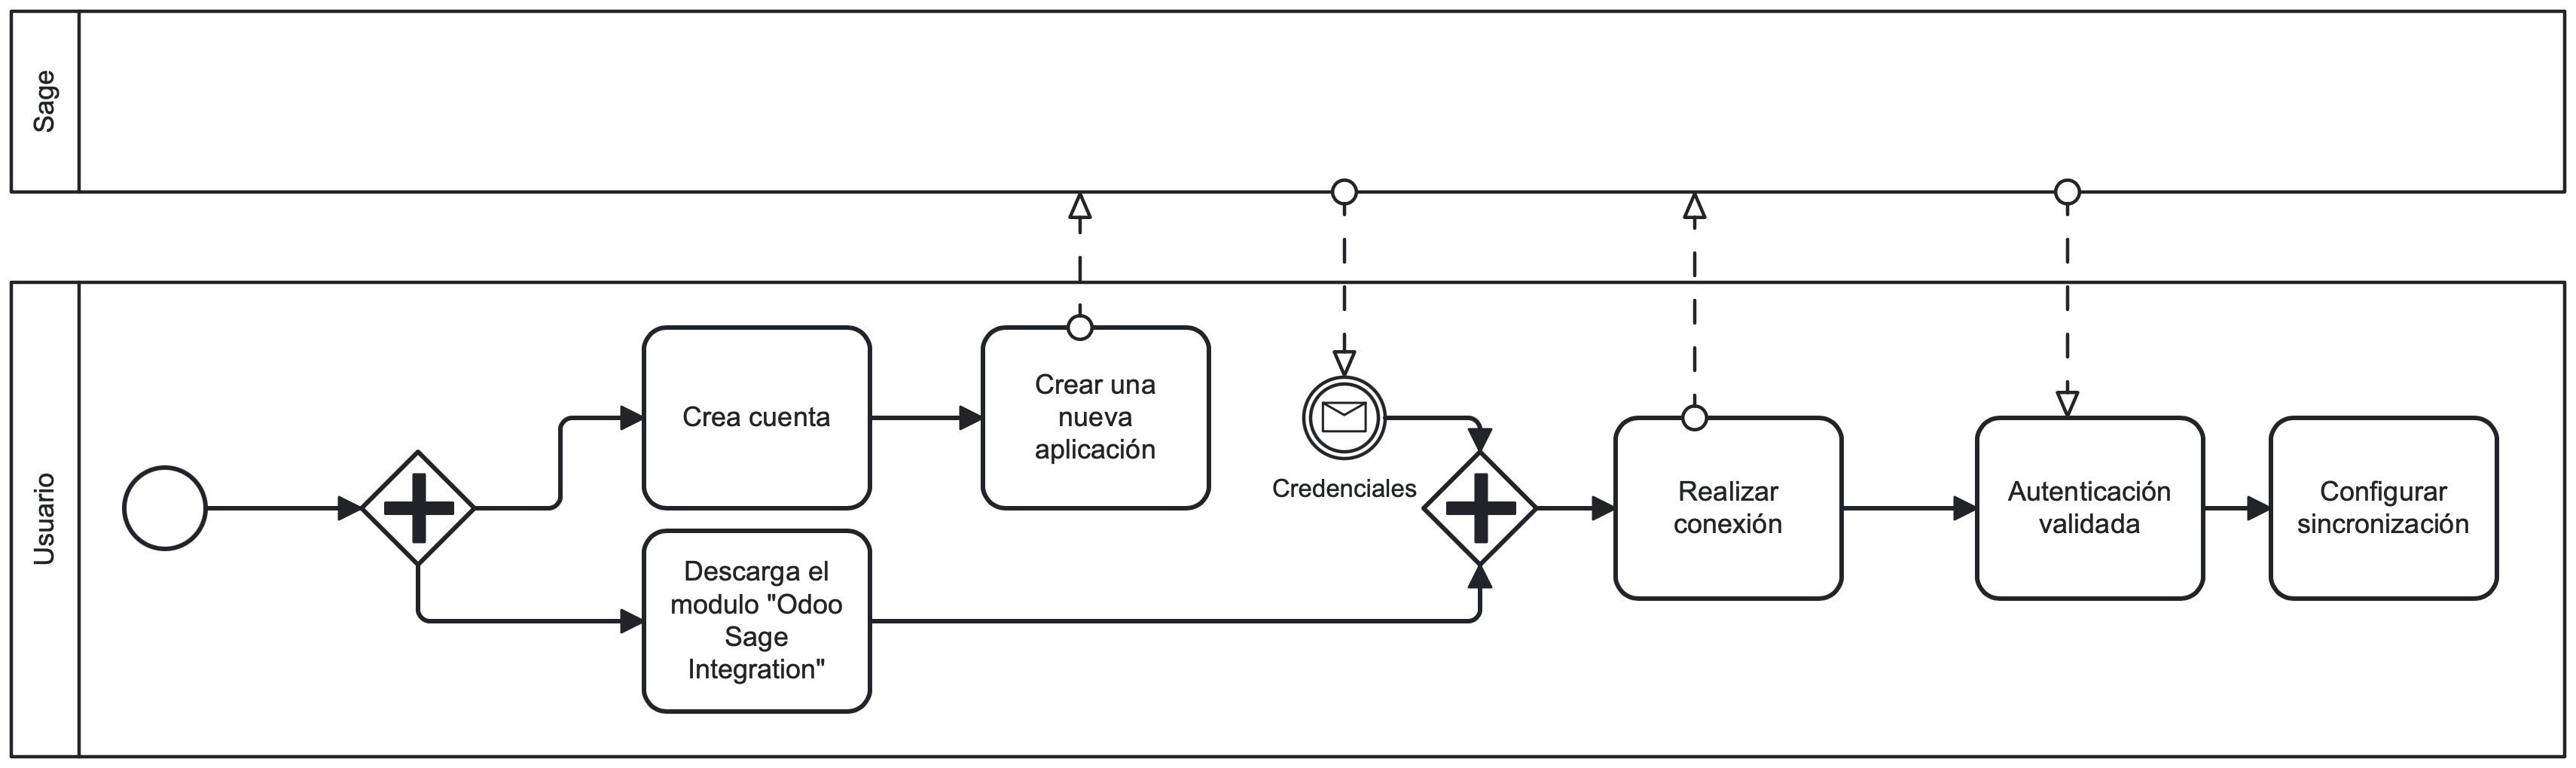
\includegraphics[width=1\linewidth]{imgConta/Fico.png}
    \caption{Diagrama BPMN 2.0 del proceso de integración de Odoo Y Sage Business Cloud}
    \label{fico}
\end{figure}

\subsection{Conclusiones}
Tras analizar el problema y las posibles soluciones externas podemos concluir:
\subsection{Conclusiones}
\paragraph{}
Basándonos en el análisis detallado realizado, las conclusiones se derivan de los siguientes puntos clave:

\begin{enumerate}
    \item \textbf{Problemas Identificados en el Módulo FICO de Odoo:} Tras un análisis exhaustivo, se han identificado varios problemas en el módulo FICO de Odoo, destacando la limitada disponibilidad de soporte para la versión 17.0, la incompletitud de la migración a español, y problemas específicos como la gestión de subvenciones y la configuración de impuestos, particularmente el IRPF. Estos problemas impactan la funcionalidad y la confiabilidad del módulo para usuarios en el contexto español.
    
    \item \textbf{Selección de Soluciones Alternativas:} Con el objetivo de resolver los problemas identificados, se han evaluado dos soluciones externas: Sage Business Cloud Contabilidad y QuickBooks. Ambas opciones ofrecen funcionalidades esenciales para la gestión contable y financiera, así como opciones de personalización. Sin embargo, se destaca la mayor complejidad de Sage Business Cloud Contabilidad y la intuitividad de QuickBooks.
    
    \item \textbf{Elección de Sage Business Cloud Contabilidad:} Después de considerar los factores mencionados, se ha decidido seleccionar Sage Business Cloud Contabilidad como la solución preferida. A pesar de su precio relativamente más alto, se valora su plataforma en la nube y el respaldo de una comunidad más amplia, lo que proporciona recursos adicionales y una mayor seguridad en la integración con el ERP existente.
    
    \item \textbf{Proceso de Integración:} Para facilitar la integración con Odoo, se utilizará el módulo Sage Integration, que simplifica la sincronización entre ambas plataformas. Se seguirán los pasos detallados proporcionados por la herramienta para establecer una conexión fluida y efectiva entre Sage Business Cloud Contabilidad y el ERP Odoo.
\end{enumerate}
\paragraph{}
En resumen, la selección de Sage Business Cloud Contabilidad como solución alternativa para los problemas identificados en el módulo FICO de Odoo se basó en una evaluación cuidadosa de las características, funcionalidades y compatibilidad con los requisitos específicos del contexto español. La elección se respalda en la confianza en la plataforma en la nube y en la comunidad detrás de Sage, así como en la facilidad de integración proporcionada por el módulo Sage Integration.

\newpage

\section{Ayuda a la toma de decisiones}
\subsection{Autoevaluación}
En esta sección se han cumplido los objetivos correspondientes al 10.
\subsection{Introducción}
\paragraph{}
 Se va a realizar una prueba del sistema Business Inteligence que ofrece Odoo para recopilar, almacenar, analizar y presentar datos de negocio con el objetivo de facilitar la toma de decisiones. Facilita la creación de informes de aspectos como finanzas, ventas e inventario, su automatización y la capacidad de añadir filtros para obtener información detallada que se desea.
\subsection{Metodología}
\paragraph{}
Para llevar a cabo una simulación del uso de Business Inteligence con Odoo se ha instalado el módulo de Tableros. Cómo se puede observar en el menú de Tableros, se han generado varios informes predefinidos que aportan información sobre las ventas, los productos, la facturación, la compra, los proveedores, el inventario y el comercio asociado a la web. 
\paragraph{}
Además, de estos informes generados en el módulo de Tableros, Odoo ofrece sistemas de Business Inteligence dentro de otros módulos y que además, se pueden incluir en la vista de Tableros. Aunque por lo general, los módulos instalados con anterioridad tienen ayudas en la visualización de la información destacan alguno de ellos. 
\paragraph{}
En el módulo CRM se puede ver una vista Kanban del flujo de ventas que aporta información de cuantas ventas hay en cada fase y los detalles de cada una, con el objetivo de ayudar a tomar decisiones sobre si realizar campañas porque llegan pocas solicitudes o si hay otro problema durante el proceso de venta. 
\paragraph{}
En el módulo de Inventario, dentro de cada producto se puede acceder a la opción de \textit{Pronóstico} donde se puede ver información sobre la cantidad del producto que hay, el que se va a vender, en qué ventas y además, se puede mostrar la información en muchas vistas adecuándose a la que se necesite. 
\paragraph{}
En el módulo de Facturación y Contabilidad, en el apartado de informes se muestran en distintos gráficos información sobre el análisis de las facturas, además, permite mostrar las facturas de manera apilada o acumulada. 
\paragraph{}
A continuación, se va a personalizar el módulo de Tableros, para ello se han establecido tres actividades de los que se quiere obtener un informe, \textit{CRM}, \textit{Ventas} e \textit{Inventario}. Dentro de cada módulo se accede al informe que se quiere añadir y pulsando en el símbolo de ajustes permite añadirlo a Tableros. Una vez realizado con las tres actividades si se accede a \textit{Mi tablero} se encontraran los tres informes generados. En este caso, el informe de \textit{CRM} aporta información sobre el flujo de ventas, información sobre la misma y en que etapa del proceso de venta se encuentra. En el informe de Ventas, se encuentra un gráfico de barras donde se muestran las ventas realizadas, a que empresa se ha realizado y el precio de la venta. Por último, se ha generado un informe del inventario en el que se muestra información sobre su estado, indicando para cada tipo de operación: recepción, traslado, fabricación y entrega, el estado de cada uno, es decir, si está en espera, retrasado o si se ha completado correctamente.
\paragraph{}
Para que los usuarios tengan informes de acuerdo con sus funciones se ha añadido el tablero desde la cuenta del propio usuario. En este caso, se ha iniciado sesión en la cuenta de Marcus que es gestor del personal de la compañía. Se ha navegado al módulo de empleados se ha activado la vista de lista y desde el icono de engranaje se ha añadido a \textit{Mis tableros}, además se ha realizado de la misma manera para el módulo de reclutamiento. Desde la cuenta de James que es responsable de ventas se ha ido al módulo de Ventas y se ha añadido como se ha explicado anteriormente la vista de todas las ventas y su estado. 
\subsection{Resultados y análisis}
\paragraph{}
Se ha instalado el módulo de Tableros de Odoo, mediante este módulo se han generado 3 informes para el Administrador. En este caso se han añadido al tablero del Administrador un informe sobre el flujo de ventas, un informe del inventario y otro del historial de ventas, vísible en la figura \ref{admin}. 
\begin{figure}[h]
    \centering
    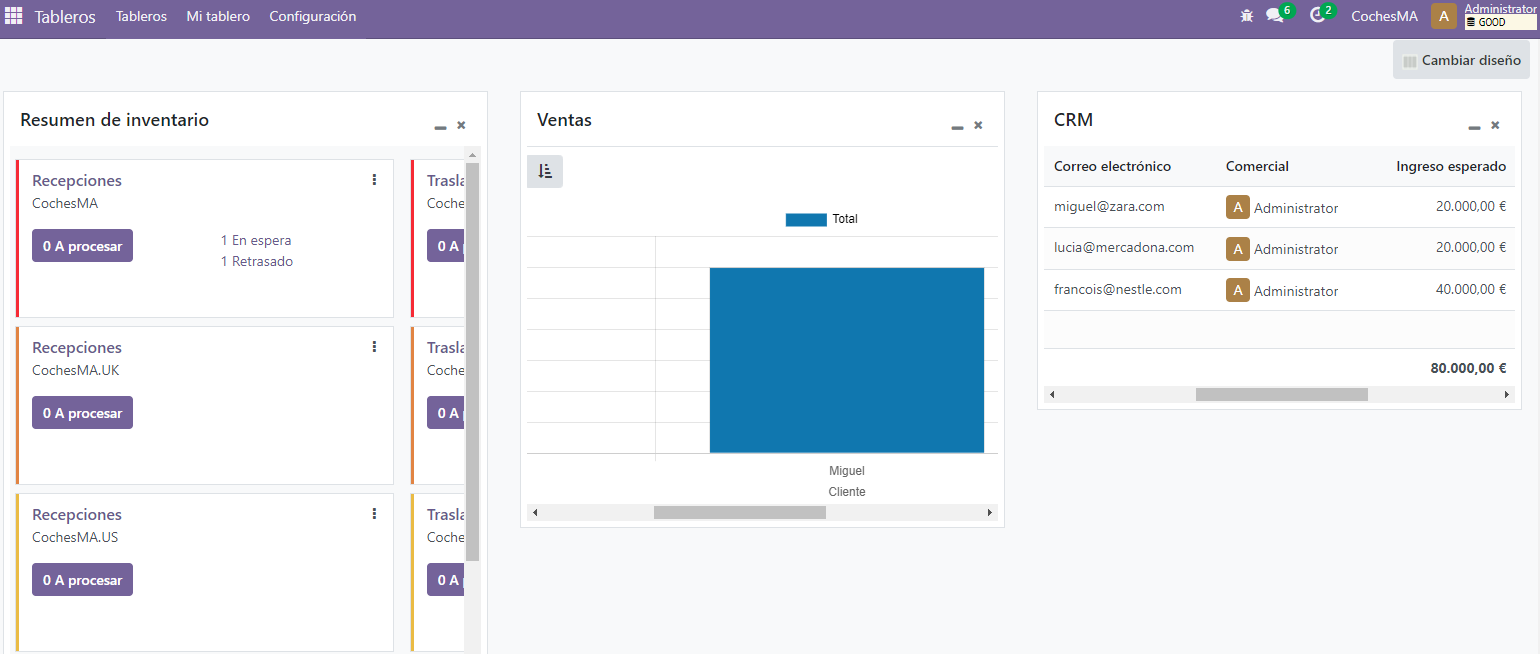
\includegraphics[width=1\linewidth]{fotosDecisiones/admin.png}
    \caption{Tablero del administrador}
    \label{admin}
\end{figure}
\paragraph{}
Además, se ha personalizado los tableros de dos usuarios, Marcus y James. Marcus es gestor de personal por lo que se le ha asignado un informe de los empleados y del reclutamiento de la empresa, porque son los que necesita un gestor de personal para analizar y ejercer sus responsabilidades, tomar decisiones estratégicas relacionadas con la gestión del talento, la contratación y los empleados, facilitando la optimización de los recursos humanos (ver figura \ref{fig:marcus}). 
\begin{figure}[h]
    \centering
    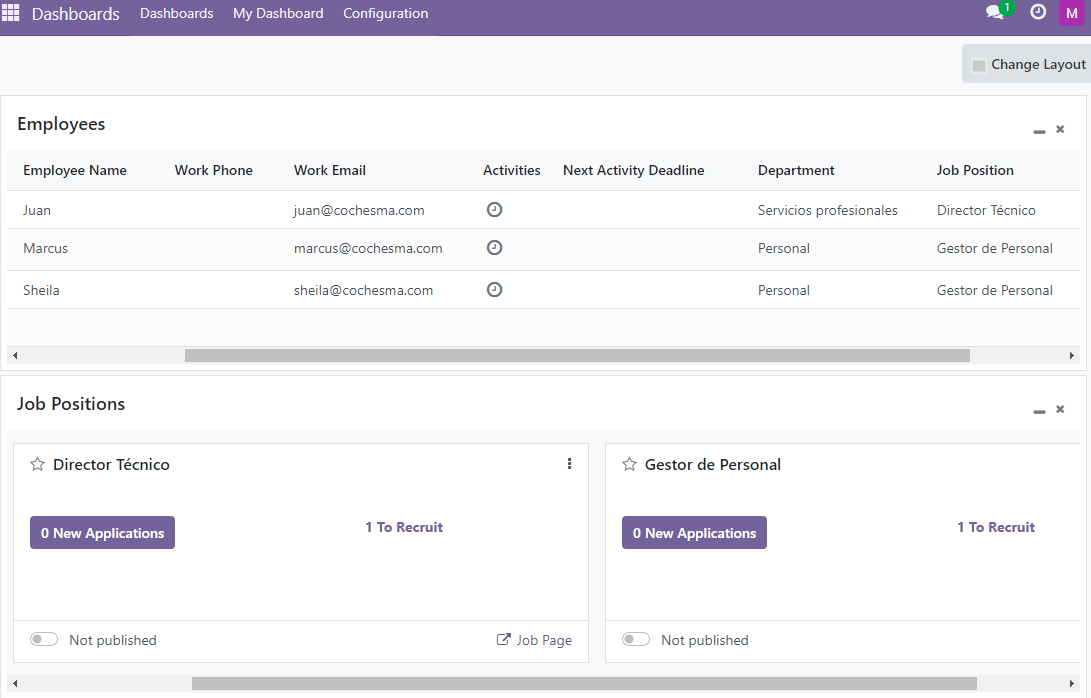
\includegraphics[width=0.9\linewidth]{fotosDecisiones/marcus.png}
    \caption{Tablero del gestor de personal Marcus}
    \label{fig:marcus}
\end{figure}
\paragraph{}
Por otro lado, a James se le ha asignado el informe de las ventas como se puede observar en la figura \ref{fig:james}, ya que proporciona una visión global del rendimiento de ventas, facilita la identificación de tendencias y contribuye a la optimización de recursos y estrategias de ventas.
\newpage
\begin{figure}[h]
    \centering
    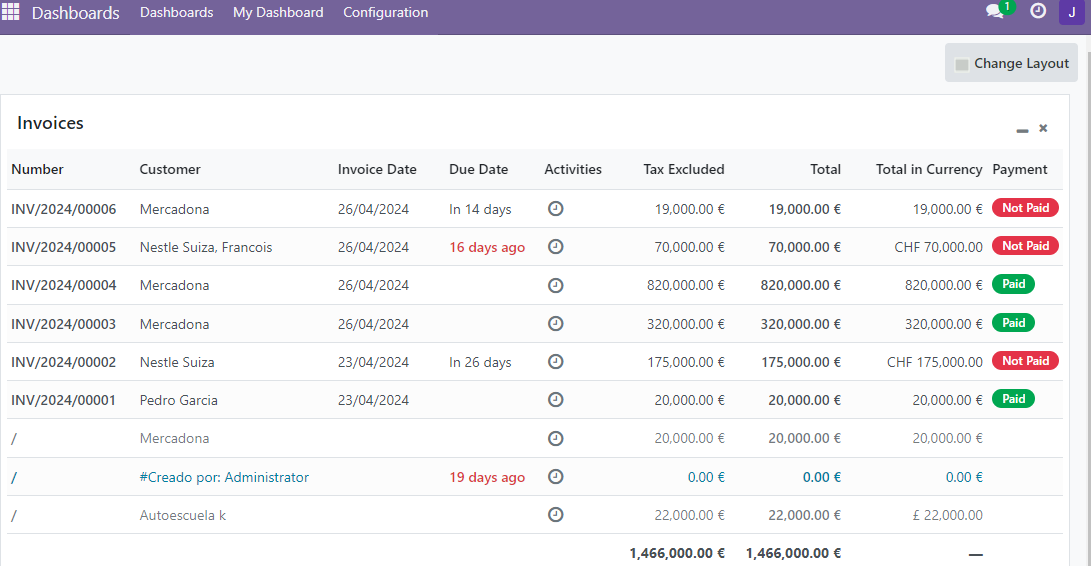
\includegraphics[width=1\linewidth]{fotosDecisiones/james.png}
    \caption{Tablero del gestor de ventas James}
    \label{fig:james}
\end{figure}
\paragraph{}
Por último, hemos modificado el diagrama BPMN \ref{fab} para representar la interacción entre el módulo de fabricación con este módulo descrito. Este nuevo diagrama es la figura \ref{bi}

\begin{figure}[h]
    \centering
    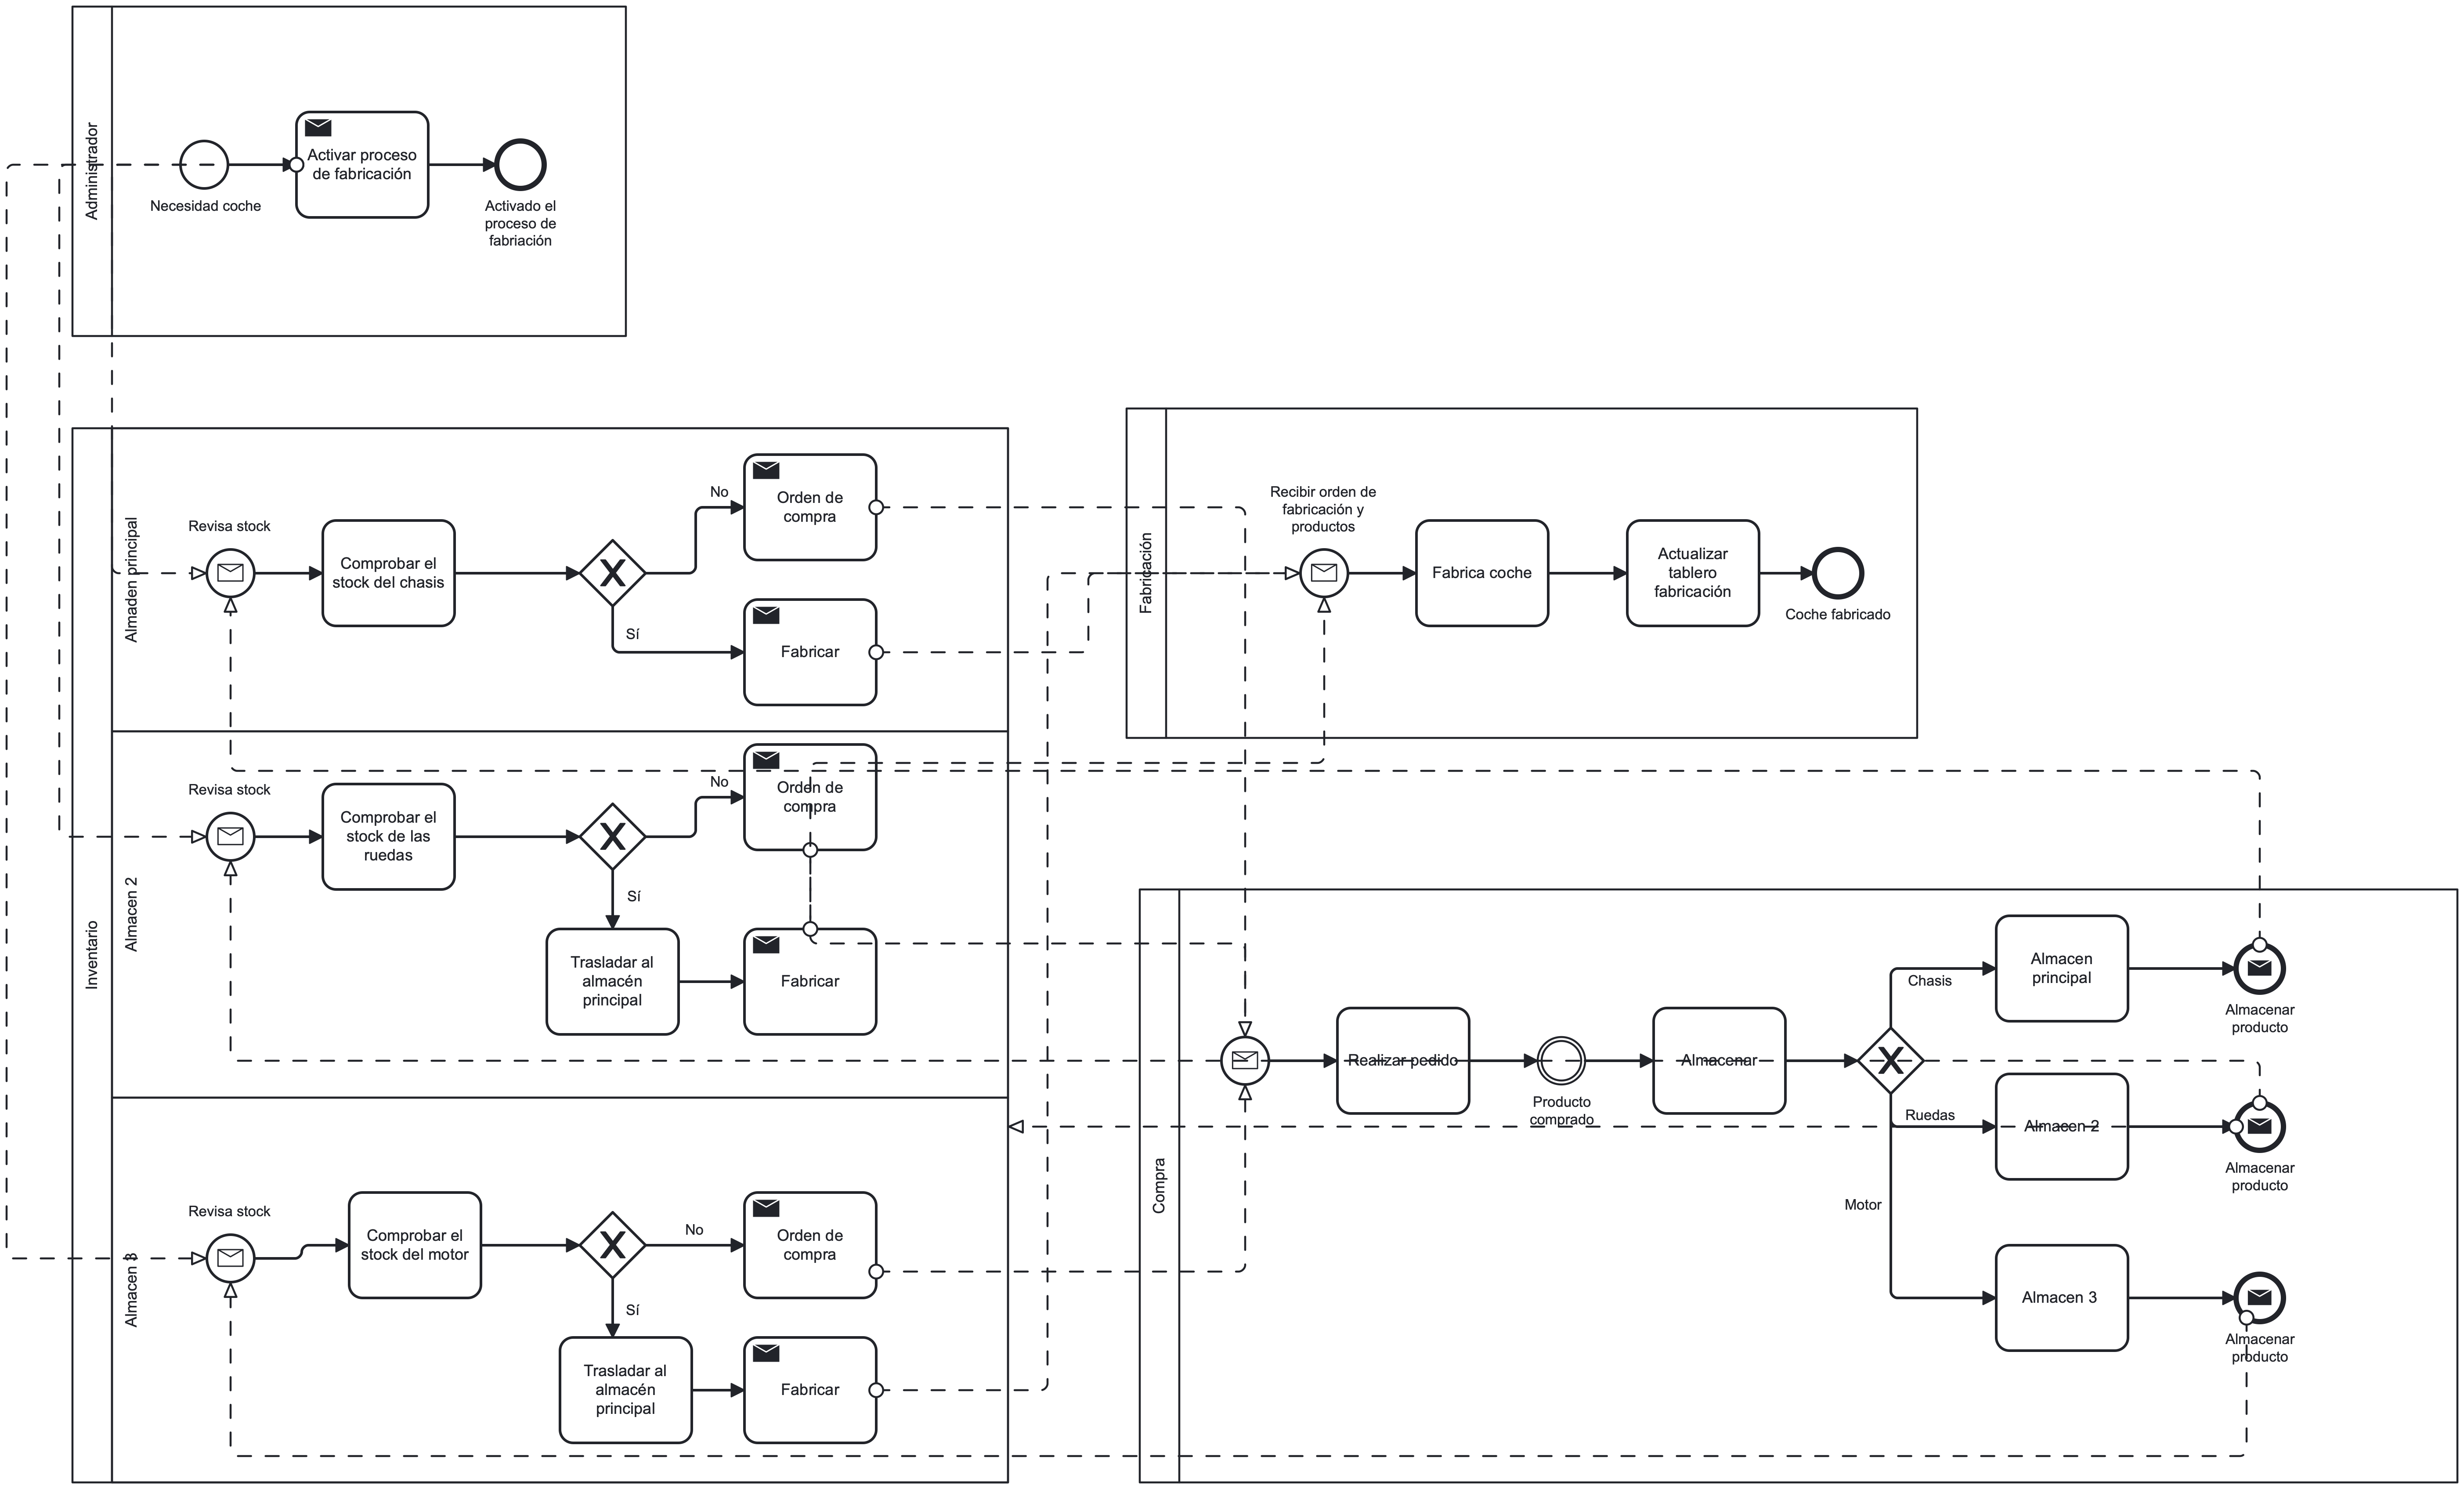
\includegraphics[width=1\linewidth]{fotosGestFab/BI.png}
    \caption{Diagrama BPMN 2.0 modificado, añadiendo la interacción con el tablero de inventario}
    \label{bi}
\end{figure}
\newpage
\subsection{Conclusiones}
\paragraph{}
Se ha logrado integrar la funcionalidad de Business Intelligence en Odoo mediante el módulo de Tableros, lo que permite a cada usuario, aprovechar los datos generados para tomar decisiones mediante la creación de dashboards personalizados. Este módulo es fácil de incorporar en Odoo, sin embargo, hay que destacar que si no se han implementado otros módulos que generen los datos necesarios, los tableros pueden perder gran parte de su valor.
\paragraph{}
Por otro lado, el módulo de Tableros proporciona una manera sencilla de personalizar la visualización de datos. No obstante, es importante mencionar que Odoo no ofrece una forma rápida de configurar Tableros, ya que es necesario acceder a cada módulo individualmente para añadir la vista, en lugar de contar con una vista centralizada donde se puedan añadir de manera más eficiente.

\newpage

\section{Gestión del conocimiento}
\subsection{Autoevaluación}
En esta sección se ha cumplido los objetivos correspondientes al 10.
\subsection{Introducción}
\paragraph{}
La gestión del conocimiento busca optimizar el uso de recursos intelectuales y promover la colaboración entre la comunidad. Para ello, se usan herramientas que tienen como objetivo compartir ideas, discutir sobre temas, plantear preguntas y colaborar en la resolución de problemas.
\subsection{Metodología}
\paragraph{}
En Odoo existe una herramienta que ofrece las características que se necesitan para la gestión del conocimiento, para obtenerlo se ha instalado el módulo de Foros. Desde el menú de sitio web en el menú de configuración se puede acceder a los Foros. Si se accede al foro de Ayuda se puede configurar la privacidad, en este caso se ha elegido que solo se accesible por usuarios conectados y también se puede configurar el modo del foro, se ha elegido que se puedan realizar conversaciones en los posts del foro. Además, se ha editado los derechos relacionados con el karma ya que se ha asignado el valor 0 a hacer preguntas y responder preguntas porque no se han verificado los correos. 
\paragraph{}
A continuación, se ha iniciado sesión con un usuario interno, se ha entrado en la página web, se ha navegado al foro y se ha seleccionado el foro de ayuda. Se ha creado una entrada al post con la pregunta correspondiente, cabe destacar que cómo el correo no está verificado el administrador tendrá que entrar al foro y validar la pregunta.
\paragraph{}
Por otro lado, se ha iniciado sesión con 5 usuarios internos diferentes y se han escrito 5 respuestas a la entrada del post. En el foro, con el objetivo de que un usuario, en este caso María, aumente su karma se ha utilizado la cuenta del administrador y se ha votado positivamente la respuesta que ha dado a una pregunta del foro. 
\paragraph{}
Además, se pueden dar insignias a los usuarios, para ello María ha realizado una pregunta en el foro y también ha escrito una respuesta. A continuación, el administrador ha validado la pregunta. El administrador desde la opción de Insignias de la configuración del modulo de Sitio Web, ha hecho clic en otorgar en la insignia de buena pregunta y la insignia de autodidacta, ambas se han asignado a María. 
\paragraph{}
Por otro lado, para probar los privilegios que tiene un usuario con mucho karma, se ha editado la ganancia de karma en el foro para que cuando recibas un voto positivo recibas 100 de karma. Desde la cuenta administrador se ha dado un voto positivo a una respuesta de María, por lo que ahora tiene más de 100 de karma. Además, se ha editado los derechos de karma y se ha asignado 100 de karma para poder editar cualquier mensaje. Por lo que María puede moderar el contenido de otros usuarios. Por último, desde la cuenta del administrador se ha creado la insignia \textit{Gurú} y se la ha otorgado a María. 
\subsection{Resultados y análisis}
\paragraph{}
Se ha conseguido configurar un foro, accesible solo por usuarios conectados y en el que se puedan hacer conversaciones.
Se ha añadido una entrada al foro de Ayuda, con la siguiente pregunta ¿Cuál es el stack tecnológico de la instalación de Odoo?. Además, otros usuarios han respondido a la pregunta con las tecnologías correspondientes. 
\newpage
\begin{figure}[h]
    \centering
    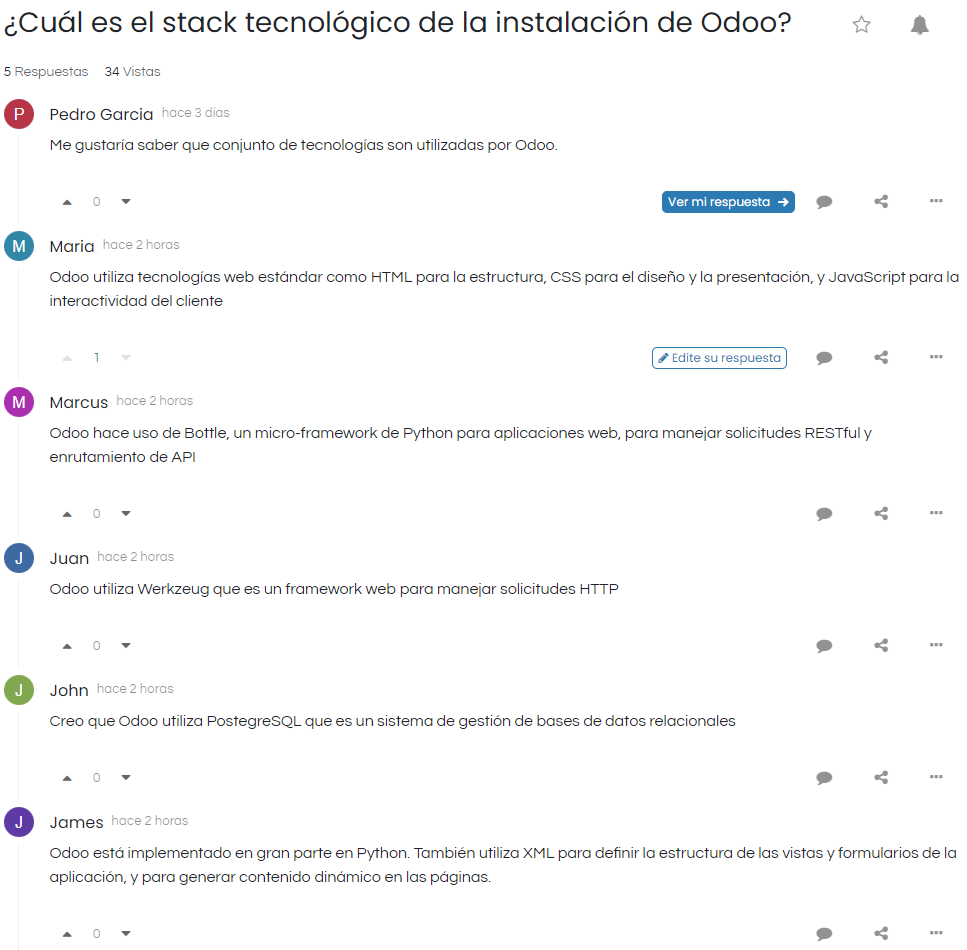
\includegraphics[width=1\linewidth]{fotosGestCon/pregunta1.png}
    \caption{La pregunta ¿Cuál es el stack tecnológico de la instalación de Odoo? en el foro}
    \label{fig:enter-label}
\end{figure}
\paragraph{}
María también ha realizado una pregunta en el foro y ha respondido en esa misma pregunta. Se ha dado un voto positivo a la respuesta de María y se le ha dado la insignia de \textit{Buena pregunta} y \textit{Autodidacta}. 
\newpage
\begin{figure}[h]
    \centering
    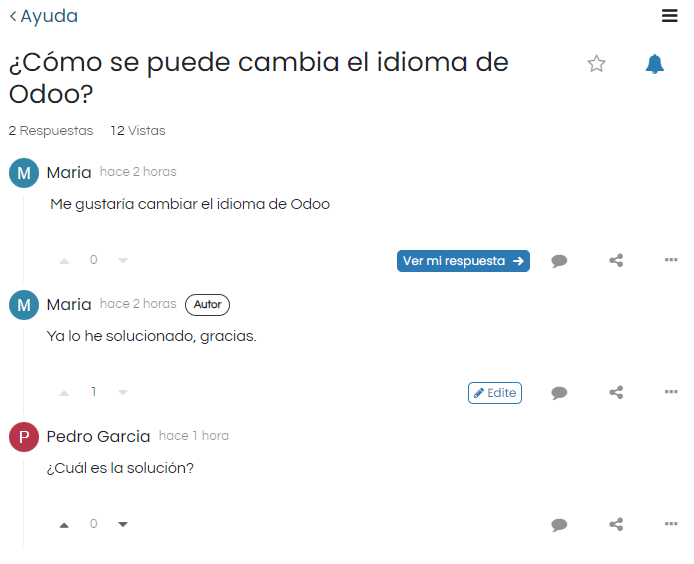
\includegraphics[width=0.75\linewidth]{fotosGestCon/pregunta2.png}
    \caption{Segunda pregunta del foro}
    \label{fig:enter-label}
\end{figure}
\begin{figure}[h]
    \centering
    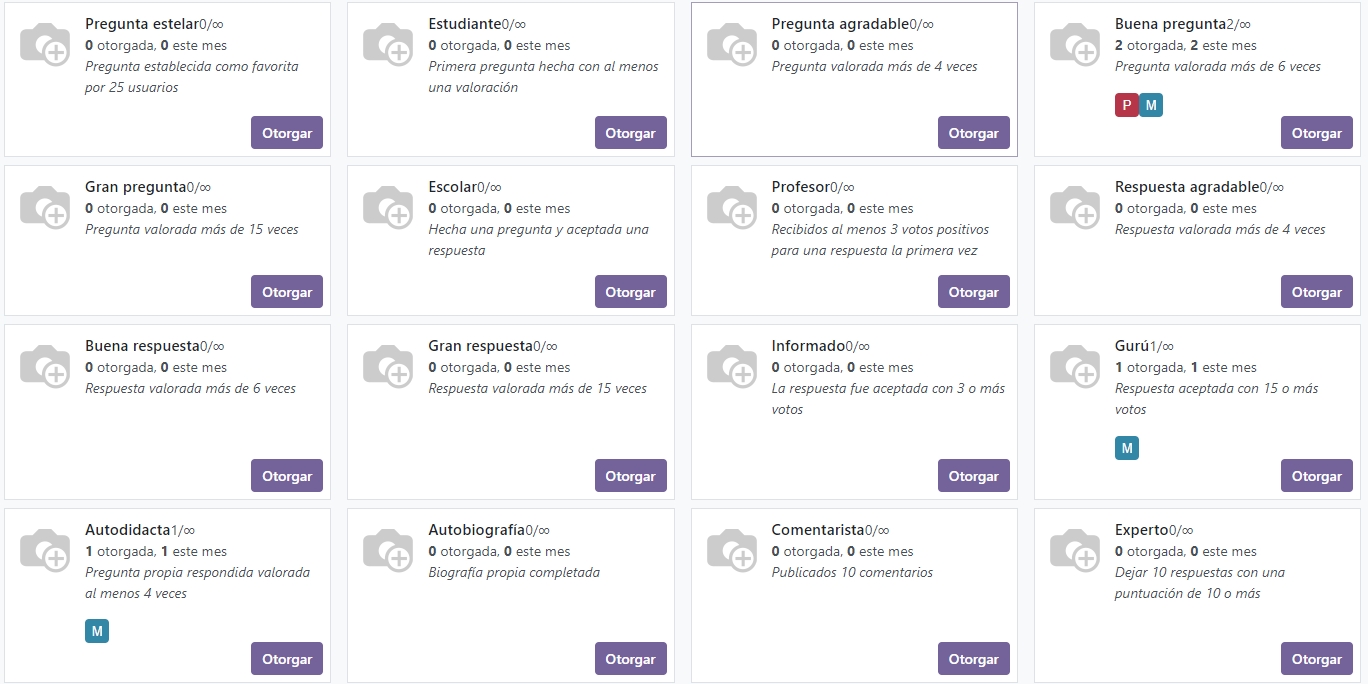
\includegraphics[width=1\linewidth]{fotosGestCon/insignias.png}
    \caption{Lista de insignias y a quién han sido otorgadas}
    \label{fig:enter-label}
\end{figure}
\paragraph{}
Por último, se ha hecho que María alcance unos puntos de karma que le permita moderar el contenido de otros usuarios y además, se le otorgado la insignia de Gurú como se puede ver en la anterior Figura.
\newpage
\begin{figure}[h]
    \centering
    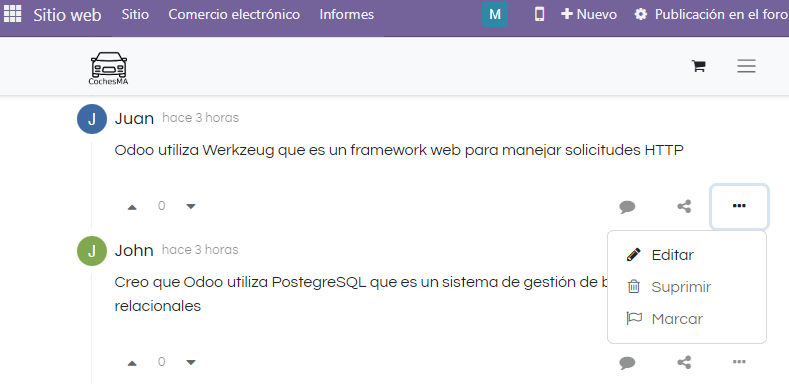
\includegraphics[width=1\linewidth]{fotosGestCon/privilegio.png}
    \caption{Capacidad de editar comentarios de otros usuarios desde la cuenta de María}
    \label{fig:enter-label}
\end{figure}
\subsection{Conclusiones}
\paragraph{}
La implementación de la herramienta de foros en Odoo ha permitido cumplir con los objetivos establecidos. Se han realizado las configuraciones necesarias de manera sencilla, ya que las acciones a realizar han sido intuitivas. 
Este módulo ha demostrado ser una herramienta efectiva para fomentar la gestión del conocimiento y la colaboración de la comunidad para mejorar la página web de la compañía. Sin embargo, deberá haber responsables que moderen el contenido de los foros para asegurar que la información es correcta y adecuada.
\newpage

\section{Elaboración de la recomendación final}
\subsection{Autoevaluación}
En esta sección se ha cumplido los objetivos correspondientes al 10
\subsection{Introducción}
Tras haber analizado los distintas funcionalidades que nos ofrece Odoo durante tres meses somos capaces de emitir una recomendación clara y fundamentada sobre la viabilidad de implementar Odoo en nuestra empresa UZ-on-Marketing. Este veredicto final es producto de una evaluación objetiva y rigurosa, considerando tanto los aspectos positivos como las limitaciones.
\subsection{Metodología}
Tras haber analizado cada uno de las distintas funcionalidades que nos ofrece Odoo; hemos evaluado cada uno de los módulos, hemos analizado las virtudes y defectos de cada uno. De esta forma, somos capaces de proporcionar una nota numérica de forma objetiva, basada en ejes de selección y determinar si cada módulo supera un umbral. Por lo tanto, previo a realizar este análisis final hemos tenido que definir cuales son los ejes de selección. Para ello, hemos decidido utilizar un estándar reconocido en la valoración de la adquisición de software. En concreto la \href{https://iso25000.com/index.php/normas-iso-25000/iso-25010}{ISO/IEC 25010}, esta decisión se ha basado en ser su amplio alcance y reconocimiento internacional. Este estándar ofrece un enfoque integral para evaluar la calidad del software en múltiples dimensiones, incluyendo características clave como funcionalidad, usabilidad, eficiencia y seguridad. Su flexibilidad y adaptabilidad lo hacen aplicable a una variedad de tipos de software, asegurando una evaluación precisa y consistente. Además, ISO/IEC 25010 se centra en las necesidades del usuario final, facilitando la comparación entre productos y garantizando la selección del software que mejor se adapte a nuestras necesidades y requisitos específicos. Esta ISO esta compuesta por 9 características de calidad, las cuales a su vez se dividen en más factores. Para realizar el análisis de este ERP hemos hecho una selección. A cada uno de los factores hemos asignado un peso y establecido unos rangos, definiendo si descartamos el software, necesitamos una segunda opición o si lo recomendamos; siendo \textless{} MAX 1/3, entre 1/3 MAX y 2/3 MAX, y \textgreater{} MAX 2/3 respectivamente. Por úlitmo hemos realizado una tabla de agregación de resultados y una conclusión.

\begin{figure}
    \centering
    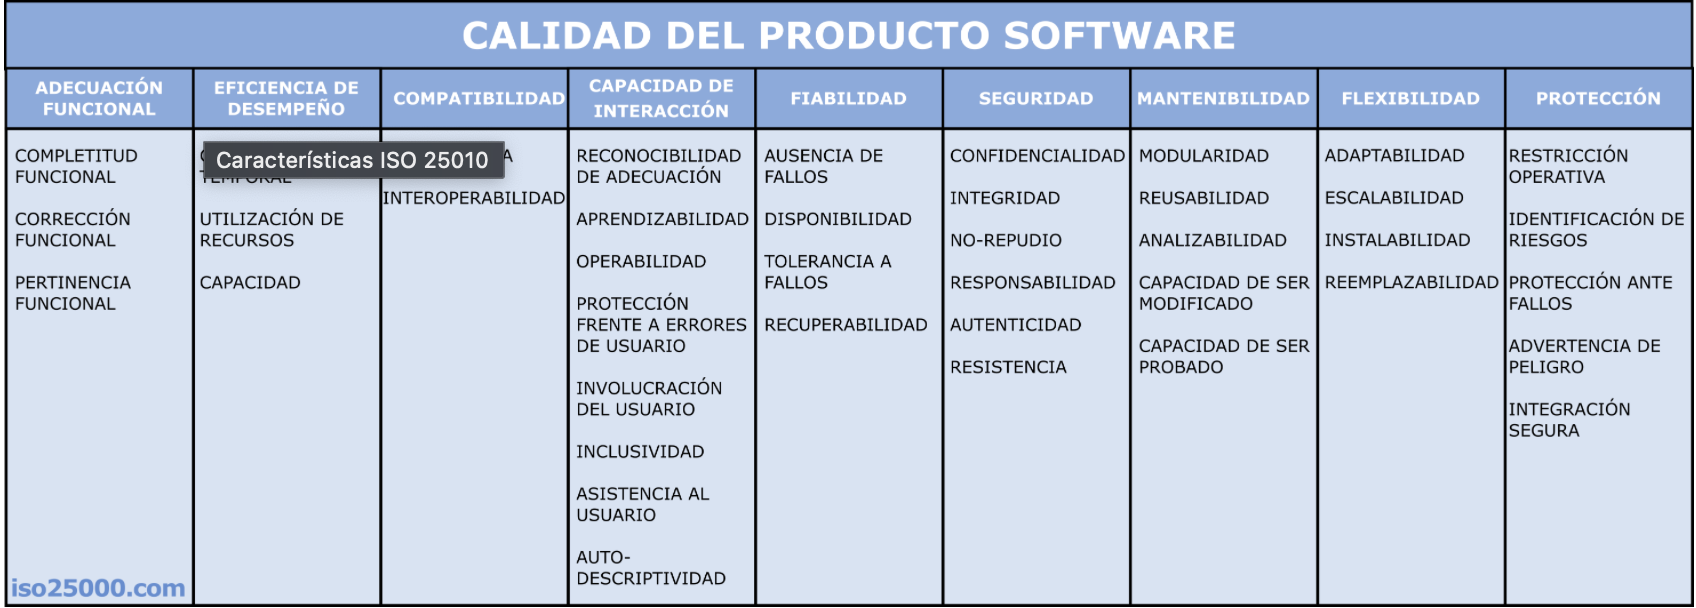
\includegraphics[width=1\linewidth]{final/iso.png}
    \caption{ISO/IEC 25010}
    \label{fig:enter-label}
\end{figure}

\subsection{Resultados y análisis}
\paragraph{}
Para hacer el análsis de Odoo y determinar si debemos adquirir hemos seleccionado 10 factores de la ISO/IEC 25010, como hemos comentado previamente.
Estos son los factores que consideramos más relevantes para Uz-on-Marketing:
\begin{itemize}
    \item \textbf{Corrección funcional}, capacidad del producto o sistema para proveer resultados exactos cuando es usado por los usuarios especificados.
    \item \textbf{Comportamiento temporal}, grado en que un producto realiza sus funciones de forma que el tiempo de respuesta y el ratio de rendimiento cumple los requisitos especificados.
    \item \textbf{Interoperabilidad}, capacidad de dos o más sistemas o componentes para intercambiar información y utilizar la información intercambiada.
    \item \textbf{Aprendizabilidad}, capacidad del producto que permite al usuario aprender su funcionamiento dentro de un tiempo especificado.
    \item \textbf{Operabilidad}, capacidad del producto que permite al usuario operarlo y controlarlo con facilidad.
    \item \textbf{Ausencia de fallos}, capacidad del sistema de llevar a cabo sus funciones sin fallos bajo condiciones normales de operación.
    \item \textbf{Confidencialidad}, capacidad de asegurar que los datos solo son accesibles a aquellos con autorización para ello.
    \item \textbf{Modularidad}, capacidad de un producto para evitar que los cambios en un componente afecten a otros componentes, pero trabajen conjuntamente entre ellos.
    \item \textbf{Instalabilidad}, facilidad con la que el producto se puede instalar y/o desinstalar de forma exitosa en un determinado entorno.
    \item \textbf{Integración segura}, capacidad de un producto para mantener la seguridad durante y después de la integración con uno o varios componentes.
\end{itemize}
\paragraph{}
A cada uno de los factores hemos asignado un peso:
\begin{table}
\centering

\begin{tblr}{
  hlines,
  vlines,
}
\textbf{Factor}                  & \textbf{Peso}  \\
Corrección funcional    & 9     \\
Comportamiento temporal & 4     \\
Interoperabilidad       & 5     \\
Aprendizabilidad        & 10    \\
Ausencia de fallos      & 8     \\
Operabilidad            & 10     \\
Confidencialidad        & 4     \\
Modularidad             & 5     \\
Instalabilidad          & 3     \\
Integración segura      & 2     \\
TOTAL                   & 60   
\end{tblr}
\caption{Tabla de los pesos asignados a cada factor}
\end{table}

\paragraph{}
El peso total obtenido es 60. Y en consecuencia, los rangos establecidos son: 
\begin{itemize}
    \item \textless{} (60*1/3 = 20) =\textgreater{} Descartamos el software
    \item entre (60*1/3 = 20) y (60*2/3 = 40 ) =\textgreater{} Necesitamos una segunda opinión 
    \item \textgreater{} (60*2/3 = 40) =\textgreater{} Recomendamos el software
\end{itemize}

Durante estos dos meses hemos estado analizando cada uno de los módulos más relevantes y que se adecuan a nuestras necesidades. Se ha evaluado objetivamente cada uno de los módulos y hemos llegado a las siguientes conclusiones de cada uno de los módulos.

\begin{itemize}
    \item Instalación: Tanto la instalación de Odoo en máquinas locales como en máquinas remotas es sencillo. Requiere ciertos conocimientos intermedios sobre administración de sistemas, sin embargo, no han surgido problemas que hayan dificultado su instalación. Se podría reconsiderar el servidor en el que alojar la máquina remota, según los intereses de la compañía.
    \item Configuración funcional, detalles y organización de la empresa: Módulo fácil de configurar aunque de gran importancia ya que será la base en la que se lleva a cabo el resto de funcionalidades.
    \item Configuración funcional, imagen corporativa: La configuración y personalización de la web pensamos que es una tarea necesaria de realizar. Además, Odoo ofrece herramientas para realizar de manera sencilla y que permiten una gran flexibilidad para adecuarla a las necesidades.
    \item Configuración técnica, copia de seguridad: Realizar copias de seguridad de la base de datos es una tarea que se puede automatizar de forma sencilla siguiendo los pasos descritos. El lugar en el que almacenarlas se podría modificar según las necesidades y recursos de la empresa.
    \item Configuración técnica, correo: Este módulo pensamos que es esencial implementarlo en Odoo ya que facilita la comunicación interna y externa, automatizando el envío de correos y ahorrando tiempo y coste a la compañía. Además, existe documentación para su configuració por lo que no debería ser díficil de implementar.
    \item Proyectos: Este módulo para nosotros es uno de los mejores que nos proporciona Odoo. Es sencillo de utilizar, intuitivo y muy útil. Nos permite gestionar las tareas de los distintos equipos de trabajo de una forma visual y eficiente. Además tiene un buen nivel de personalización. 
    \item Gestión de producción (MRP): En este apartado se gestiona una funcionalidad que referencia una actividad esencial dentro de la empresa. Sin embargo, se han encontrado problemas para realizar la configuración completa de los módulos ya que la automatización de los módulos es una tarea compleja y que requiere una cantidad considerable de tiempo para su correcto funcionamiento.  
    \item Relación con clientes (CRM): En cuanto a este módulo es una tarea compleja pero que se ha podido implementar relativamente rápido ya que aunque tenga muchas posibilidades en su configuración es intuitivo.
    \item Gestión de personal (HR): Módulo importante en la gestión de una empresa. Se ha configurado de manera sencilla. Cabe destacar que pensamos que esta funcionalidad no es muy escalable si el número de empleados aumenta considerablemente.
    \item Contabilidad y finanzas (FICO): Odoo 17.0 tiene un gran problema con este módulo y se tiene que recurrir a software externo para resolverlo. Su implementación no aparenta ser sencilla, dado sugerido no es oficial y no asegura que se pueda completar esta tarea con éxito. Existen otras alternativas que se podrían analizar en caso de necesidad.
    \item Business Intelligence: Este módulo permite la visualización de los diferentes ámbitos de la compañía de una manera adecuada. Sin embargo, no aporta una gran mejora en su objetivo ya que lo que hace es centralizar la información que ya se visualizaba en los demás módulos.
    \item Gestión del conocimiento: Este módulo tiene una gran importancia ya que permite 
\end{itemize}

\paragraph{}
Por último hemos realizado una tabla de agregación de resultados (Cuadro \ref{tabla-agre}) en la cual se analizado objetivamente este software.
% \usepackage{tabularray}



\begin{table}
\centering
\caption{Tabla de los pesos asignados a cada factor}
\begin{tabular}{|l|l|l|l|} 
\hline
\textbf{Factor}         & \textbf{Peso} & \textbf{Ooo 17.0} & \textbf{Observaciones}                                                                                                                                                                                                                                          \\ 
\hline
Corrección funcional    & 9             & Sí                & \begin{tabular}[c]{@{}l@{}}Durante su uso el producto ha funcionado correctamente~\\y se ha podido lograr los objetivos.\end{tabular}                                                                                                                           \\ 
\hline
Comportamiento temporal & 4             & Sí                & \begin{tabular}[c]{@{}l@{}}La respuesta a la hora de interactuar con el sistema\\es rápida. Salvo a la hora de actualizar información, se debe \\hacer manualmente y no es instantáneo~\end{tabular}                                                            \\ 
\hline
Interoperabilidad       & 5             & Sí                & \begin{tabular}[c]{@{}l@{}}Los distintos módulos están constantemente compartiendo \\información entre ellos y cualquier cambio en uno de \\ellos provoca modificaciones en el resto\end{tabular}                                                               \\ 
\hline
Aprendizabilidad        & 10            & No                & \begin{tabular}[c]{@{}l@{}}Se ha trabajado de forma simultánea en \\módulos separados y los cambios realizados \\en cada módulo se actualizaba al instante.\end{tabular}                                                                                        \\ 
\hline
Ausencia de fallos      & 8             & Sí                & \begin{tabular}[c]{@{}l@{}}Durante los tres meses de pruebas no han \\aparecido errores significativos en el comportamiento~\end{tabular}                                                                                                                       \\ 
\hline
Operabilidad            & 10            & No                & \begin{tabular}[c]{@{}l@{}}Su interfaz es poco intuitiva en gran parte de módulos \\ y provoca que la curva \\~de aprendizaje es demasiado pronunciada. Además,\\ durante estos meses nos ha costado realizar ciertas \\tareas al no encontrar fácilmente en la interfaz\end{tabular}  \\ 
\hline
Confidencialidad        & 4             & Sí                & \begin{tabular}[c]{@{}l@{}}Los datos están accesibles únicamente por las \\personas que tienen permisos\end{tabular}                                                                                                                                            \\ 
\hline
Modularidad             & 5             & Sí                & \begin{tabular}[c]{@{}l@{}}Odoo está formado por una gran cantidad de \\módulos independientes que a su vez cooperan\\~para potenciar sus funcionalidades\end{tabular}                                                                                          \\ 
\hline
Instalabilidad          & 3             & Sí                & \begin{tabular}[c]{@{}l@{}}La instalación y configuración técnica es relativamente\\sencillo\end{tabular}                                                                                                                                                       \\ 
\hline
Integración segura      & 2             & Sí                & No se han encontrado problemas                                                                                                                                                                                                                                  \\ 
\hline
\textbf{TOTAL}          & 60            & 40                &                                                                                                                                                                                                                                                                 \\
\hline
\end{tabular}
\caption{Tabla de agregación de resultados}
\label{tabla-agre}
\end{table}

\paragraph{}
Tras analizar si el software analizado cumple cada uno de los factores relevantes para la empresa obtenemos un total de 40. Lo que significa que se encuentra en el segundo intervalo entre 20 y 40. Lo que significa que se debería consultar con otro experto para tomar la decisión. 
\subsection{Conclusiones}
\paragraph{}
Tras varios meses realizando la evaluación del software de Odoo hemos descubierto un software que no permite gestionar nuestra empresa en su totalidad, desde la contratación de personal hasta la organización de nuestro inventario. Odoo tiene sus puntos fuertes y otros no tan buenos. Durante la realización de pruebas sistemáticas considerábamos que este software no era adecuado para nuestra empresa, sin embargo, al realizar una evaluación objetiva y analizando diversos factores que engloban las necesidades de la empresa, UZ-on-Marketing. La explicación a este descontento durante la evaluación con este ERP se debe a la pronunciada curva de aprendizaje y la complejidad de este software para un persona que nunca ha utilizado un sistema de información similar a este. A pesar de estos factores, las funcionalidades que nos brinda este software son muy beneficiosas para nuestras necesidades. La tabla de resultados nos ha permitido realizar una evaluación totalmente objetiva y dejando de lado nuestras percepciones y opiniones.

\paragraph{}
Por lo tanto, objetivamente hemos obtenido una puntuación de 40 sobre 60. Esto significa que se encuentra en el segundo rango, muy cerca del tercero. Siguiendo el criterio obtenido, se debería consultar con otro experto para estar completamente seguros en la decisión final. Sin embargo, consideramos que este valor está muy cerca del ultimo rango. Por lo tanto, recomendamos adquirir este software, siempre y cuando se contrate un experto o se realice una formación previa a los trabajadores para reducir el tiempo de aprendizaje. Y de esta forma, subsanamos las carencias obtenidas en la tabla de agregación de resultados.
\newpage


\section{Bibliografía}
\begin{enumerate}
    \item \href{https://www.docker.com}{Docker}
    \item \href{https://aws.amazon.com}{Amazon Web Service}
    \item \href{https://aws.amazon.com/es/training/ramp-up-guides/}{Guías de estudio de AWS}
    \item \href{https://azure.microsoft.com/en-us/}{Microsoft Azure}
    \item \href{https://railway.app}{Railway.app}
    \item \href{https://www.odoo.com/es_ES}{Web oficial de Odoo}
    \item \href{https://chatgpt.com}{ChatGPT 3.5}
    \item \href{https://iso25000.com/index.php/normas-iso-25000/iso-25010}{ISO 25010}
    \item \href{https://quickbooks.intuit.com/eu/}{quickbooks}
    \item \href{https://www.sage.com/es-es/}{Sage}
    \item \href{https://www.lucidchart.com/pages/es/bpmn-bpmn-20-tutorial}{Tutorial de BPMN y BPMN 2.0}
    \item \href{https://www.digitalocean.com/community/tutorials/how-to-create-a-self-signed-ssl-certificate-for-nginx-in-ubuntu-20-04-1}{How To Create a Self-Signed SSL Certificate for Nginx in Ubuntu 20.04}
    \item \href{https://apps.odoo.com/apps/modules/14.0/odoo_sage_integration/}{Odoo Sage Integration}
    \item \href{https://github.com/OCA/l10n-spain/issues}{OCA/l10n-spain issues}
    \item \href{https://www.youtube.com/watch?v=zQyrhjEAqLs}{Curso de AWS Desde Cero | Amazon Web Services} [video]
    \item \href{https://www.odoo.com/documentation/15.0/es/applications/general/email_communication/google_oauth.html}{Conectar Gmail con Odoo mediante Google OAuth}    
\end{enumerate}
\end{document}

